%%%%%%%%%%%%%%%%%%%%%%%%%%%%%%%%%%%%%%%%%%%%%%%%%%%%%%%%%%%%%%%%%%%%%%%%%%
%%%%%                         CHAPITRE 1                            %%%%%%
%%%%%%%%%%%%%%%%%%%%%%%%%%%%%%%%%%%%%%%%%%%%%%%%%%%%%%%%%%%%%%%%%%%%%%%%%%

\lhead[\fancyplain{}{\leftmark}]%Pour les pages paires \bfseries
      {\fancyplain{}{}} %Pour les pages impaires
\chead[\fancyplain{}{}]%
      {\fancyplain{}{}}
\rhead[\fancyplain{}{}]%Pour les pages paires 
      {\fancyplain{}{\rightmark}}%Pour les pages impaires \bfseries
\lfoot[\fancyplain{}{}]%
      {\fancyplain{}{}}
\cfoot[\fancyplain{}{\thepage}]%\bfseries
      {\fancyplain{}{\thepage}} %\bfseries
\rfoot[\fancyplain{}{}]%
     {\fancyplain{}{\scriptsize}}


%%%%%%%%%%%%%%%%%%%%%%%%%%%%%%%%%%%%%%%%%%%%%%%%%%%%%%%%%%%%%%%%%%%%%%%%%%
%%%%%                      Start part here                          %%%%%%
%%%%%%%%%%%%%%%%%%%%%%%%%%%%%%%%%%%%%%%%%%%%%%%%%%%%%%%%%%%%%%%%%%%%%%%%%%

\chapter{Contexte industriel et problématique de recherche}
\label{ch:objectives}

%==============================================================================	Résumé du chapitre

\begin{center}
\rule{0.7\linewidth}{.5pt}
\begin{minipage}{0.7\linewidth}
\smallskip

Dans ce premier chapitre, nous présentons le contexte du procédé d'injection-moulage des thermoplastiques dans lequel s'inscrit nos travaux.
Dans un premier temps, nous étudierons les problématiques de recherche de la littérature en injection-moulage.
Dans un second temps, nous positionnerons notre travail sur la problématique du  du contrôle de la qualité géométrique et d'aspect en temps de cycle industriel.

%\smallskip
\end{minipage}
\smallskip
\rule{0.7\linewidth}{.5pt}
\end{center}

\minitoc
\newpage

\section{Le procédé d'injection-moulage des thermoplastiques}  \label{sec:molding_presentation}
% Notre travail s'inscrit dans le cadre du projet de recherche collaboratif FUI SAPRISTI, qui cherche à optimiser le procédé d'injection-moulage des thermoplastiques.
% Dans cette première section, nous présenterons ce procédé de mise en forme des pièces par moulage d'un thermoplastique.

\begin{figure}[bthp]
	\centering
	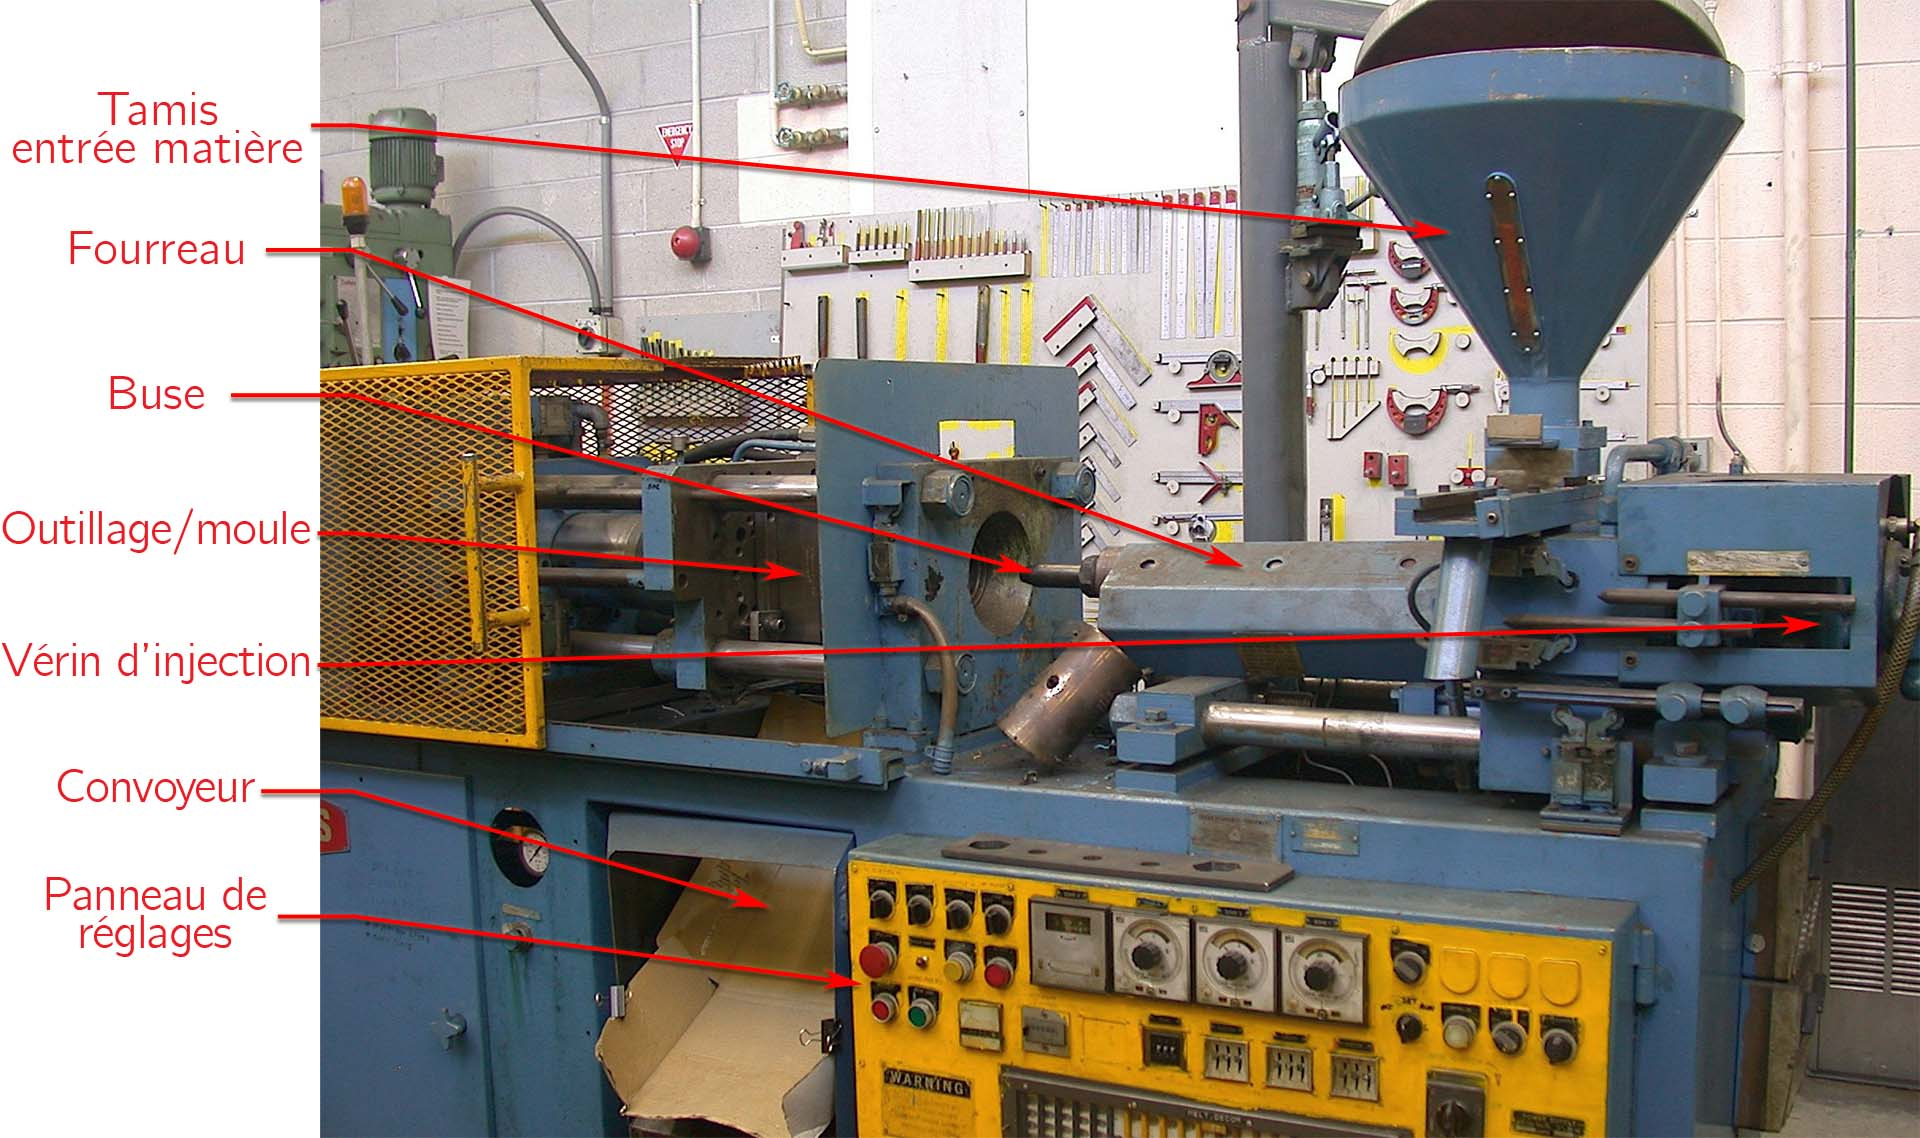
\includegraphics[width=0.8\textwidth,height=\textheight,keepaspectratio]{../Chap1/Figures/PlasticsInjectionMoulderJones_annotee.jpg}
	\caption[Une presse à injecter.]{Une presse à injecter. Photographie originale de \href{https://commons.wikimedia.org/wiki/File:PlasticsInjectionMoulderJones.jpg}{Glenn McKechnie \ccLogo \ by SA \textnormal{2.5}, Wikimedia Commons}.}
	\label{fig:PlasticsInjectionMoulderJones}
\end{figure}

% \subsection{Présentation du procédé d'injection-moulage des thermoplastiques}
La machine qui met en œuvre le procédé d'injection-moulage est la presse à injecter (voir la Figure \ref{fig:PlasticsInjectionMoulderJones}).
Un polymère est fondue dans un tube chauffé, appelé le fourreau.  % est au dessus de son point de fusion qui 
Le fourreau contient une vis pour malaxer la matière.  % et la "plastifier".
Dans une presse à injecter, on distingue deux parties cinématiques indépendantes : la vis de dosage et l'outillage amovible.
La rotation et l'avance de la vis sont régulées afin de définir les caractéristiques de la matière fondue qui sera injectée.
En particulier, il s'agit d'homogénéiser la matière fondue afin qu'elle ait une certaine viscosité.
L'avancée de la vis produit une pression sur la matière qui est également régulée : c'est la pression d'injection.
Le procédé d’injection-moulage des thermoplastiques consiste à injecter sous une pression élevée, généralement supérieure à 100 MPa, le polymère fondu et visqueux dans un moule.
La pression est maintenue pendant le refroidissement de la matière ; en particulier jusqu'à ce que le canal par lequel la matière est entrée dans le moule soit solidifié.

Cette phase de maintien permet de densifier la matière afin de compenser le retrait consécutif au refroidissement.
Le passage de la phase d'injection à la phase de maintien est appelé la commutation (on parle couramment de "point de commutation").
La phase de maintien se termine avant le début de la phase d'injection.
La phase de dosage, qui est réalisée pendant le moulage d'une pièce, conditionne les caractéristiques de la matière fondue pour la pièce suivante ; il y a un cycle de décalage.

L'ensemble qui constitue le moule est appelé un "outillage" ; ce dernier intègre un système de régulation thermique à température constante afin de favoriser le refroidissement de la pièce.
L'outillage doit également supporter les contraintes mécaniques des pressions d'injection et l'on cherche à éviter la déformation de sa géométrie pendant l'injection.
C'est pourquoi les outillages en injection-moulage sont volumineux et massifs en comparaison des dimensions des pièces produites.

% TODO: reprendre le schéma-bloc pour Éric
\begin{figure}[hbtp]
	\centering
	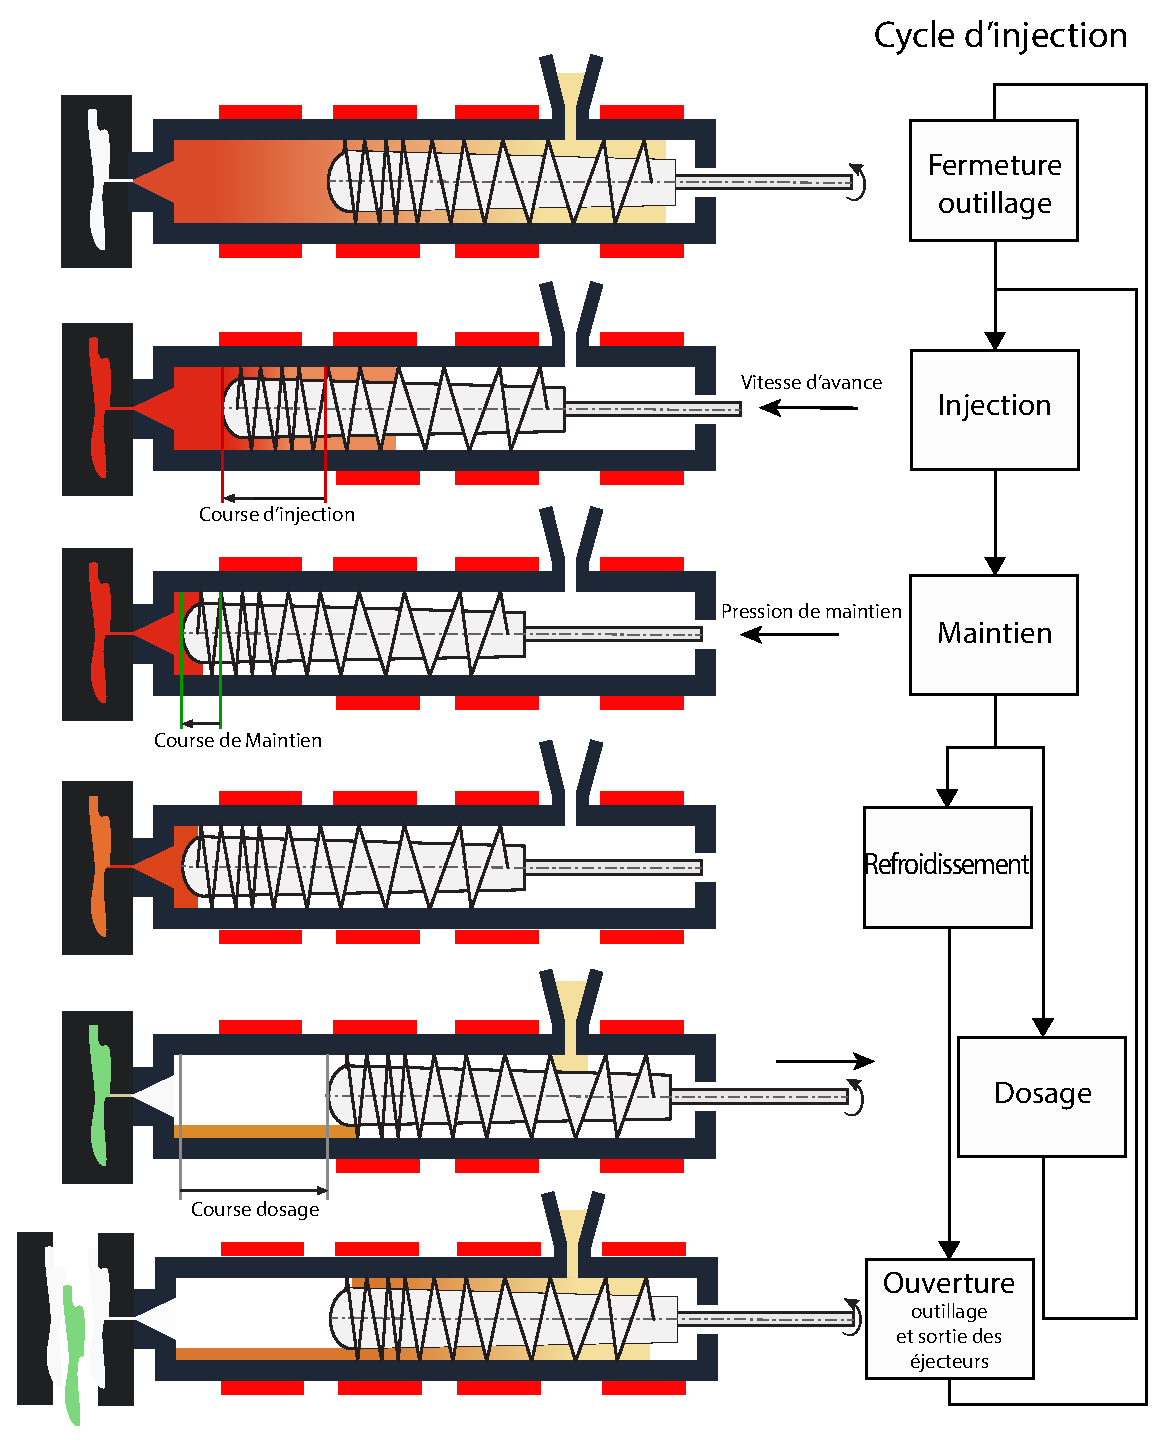
\includegraphics[width=0.9\textwidth,height=\textheight,keepaspectratio]{../Chap1/Figures/SAPRISTI_Schema-cycle.pdf}
	\caption{Schéma-bloc du procédé d'injection-moulage.}
	\label{fig:cycle_injection}
\end{figure}

Le procédé d'injection-moulage des thermoplastiques est un procédé cyclique.
Afin de mettre en évidence la séquence d’un cycle du procédé, nous proposons un schéma bloc d’un cycle d’injection en Figure \ref{fig:cycle_injection}.
On remarque en particulier que l'étape de dosage est réalisé en parallèle du refroidissement de la pièce et de son éjection.
Le dosage est l'étape pendant laquelle la matière première est fondue dans la vis d'injection.
% C'est une étape clé car il est nécessaire de garantir une certaine viscosité de la matière fondue.
% À cause de l'étape de dosage, la production d'une pièce est conditionnée par la production de la pièce précédente.
Lors du démarrage d'une presse à injecter, il est courant de produire une vingtaine de pièce pour ajuster les réglages et stabiliser le cycle.
Nous détaillons dans la Section \ref{subsec:process_parameters} suivante les paramètres qui peuvent être réglés sur une presse à injecter.

Le procédé d'injection-moulage est également séquentiel : il est composé de phases successives (voir Figure \ref{fig:cycle_injection}).
Chaque phase possède des paramètres qui influent sur les phases suivantes et, à terme, sur les caractéristiques du produit fini.
Les multiples phases font que le nombre de paramètres qui peuvent être ajustés sur le procédé est supérieur à vingt.
Il est possible d’ajuster précisément les températures, les courbes de pressions et les durées d’ouvertures et de fermetures de multiples canaux d’injection.  % buses d’injection.
% Ainsi, l’espace des variables de pilotage est grand et les variables sont continues.
Enfin, le procédé d'injection-moulage possède une certaine dynamique : c'est à dire que l'ajustement d'un des paramètres du procédé met une certaine durée avant de se répercuter sur les produits.
Cette dynamique est majoritairement due à l'inertie thermique de l'outillage massif.

% refroidi ; à maintenir une pression de compactage pendant une durée spécifique; puis à éjecter la pièce tout en préparant en parallèle la matière nécessaire au cycle suivant. 

% Relecture Éric
% Présenter les contraintes du procédé d'injection
% -> Réglage initial du point de fonctionnement difficle
% -> Peu de dérive du procédé, causes exceptionnelles de Shewart
% -> Pas ou peu de mesure de la qualité en ligne de production, pourquoi ? -> introduire notre travail

D'un point de vue industriel, l’injection-moulage des thermoplastiques est un procédé à haute cadence, peu coûteux car répétable.
Une fois la presse à injecter réglée, le procédé est généralement stable dans le temps.
Il peut produire de manière continue plusieurs milliers de pièces sans intervention humaine.
De plus, le coût de la matière première thermoplastique est faible.

La pratique industrielle de la production d'une pièce par moulage de thermoplastique suit les étapes suivantes :
\begin{enumerate}
	\item Apport de la matière première
	\item Injection-moulage de la pièce
	\item Stockage des pièces
	\item Étapes de finition (traitements de surface, peintures) 
	\item Stockage des pièces
	\item Contrôle de la qualité
	\item Expédition
\end{enumerate}
Le contrôle de la qualité des pièces n'est aujourd'hui pas réalisé dès la sortie du moule (après l'étape 2.).
Ainsi, si une pièce est non-conforme après l'étape d'injection-moulage, elle ne sera pas écartée de la chaîne de production.
Nous discuterons en particulier dans la Section \ref{sec:research_objectives} des limites qui contraignent la réalisation du contrôle en ligne de production.
% ; puis nous présenterons les objectifs de recherche de notre travail de doctorat concernant ce point.

\subsection{Paramètres réglables d'une presse à injecter} \label{subsec:process_parameters}

Le nombre de paramètres réglables d'une presse à injecter est grand.
Dans le Tableau \ref{tab:process_parameters}, nous répertorions les 16 paramètres les plus courants qui peuvent être réglés sur un presse.
Cette liste n'est pas exhaustive.
En particulier, les choix de la matière première, de la buse et les profils d'évolution des pressions ajoutent de nombreuses possibilités de réglage.
Nous remarquons que de nombreux paramètres sont dépendants.
Par exemple, la durée du cycle de production dépend de la vitesse d'injection, qui dépend également de la pression d'injection que l'ont souhaite obtenir.

\begin{figure}[bthp]
	\centering
	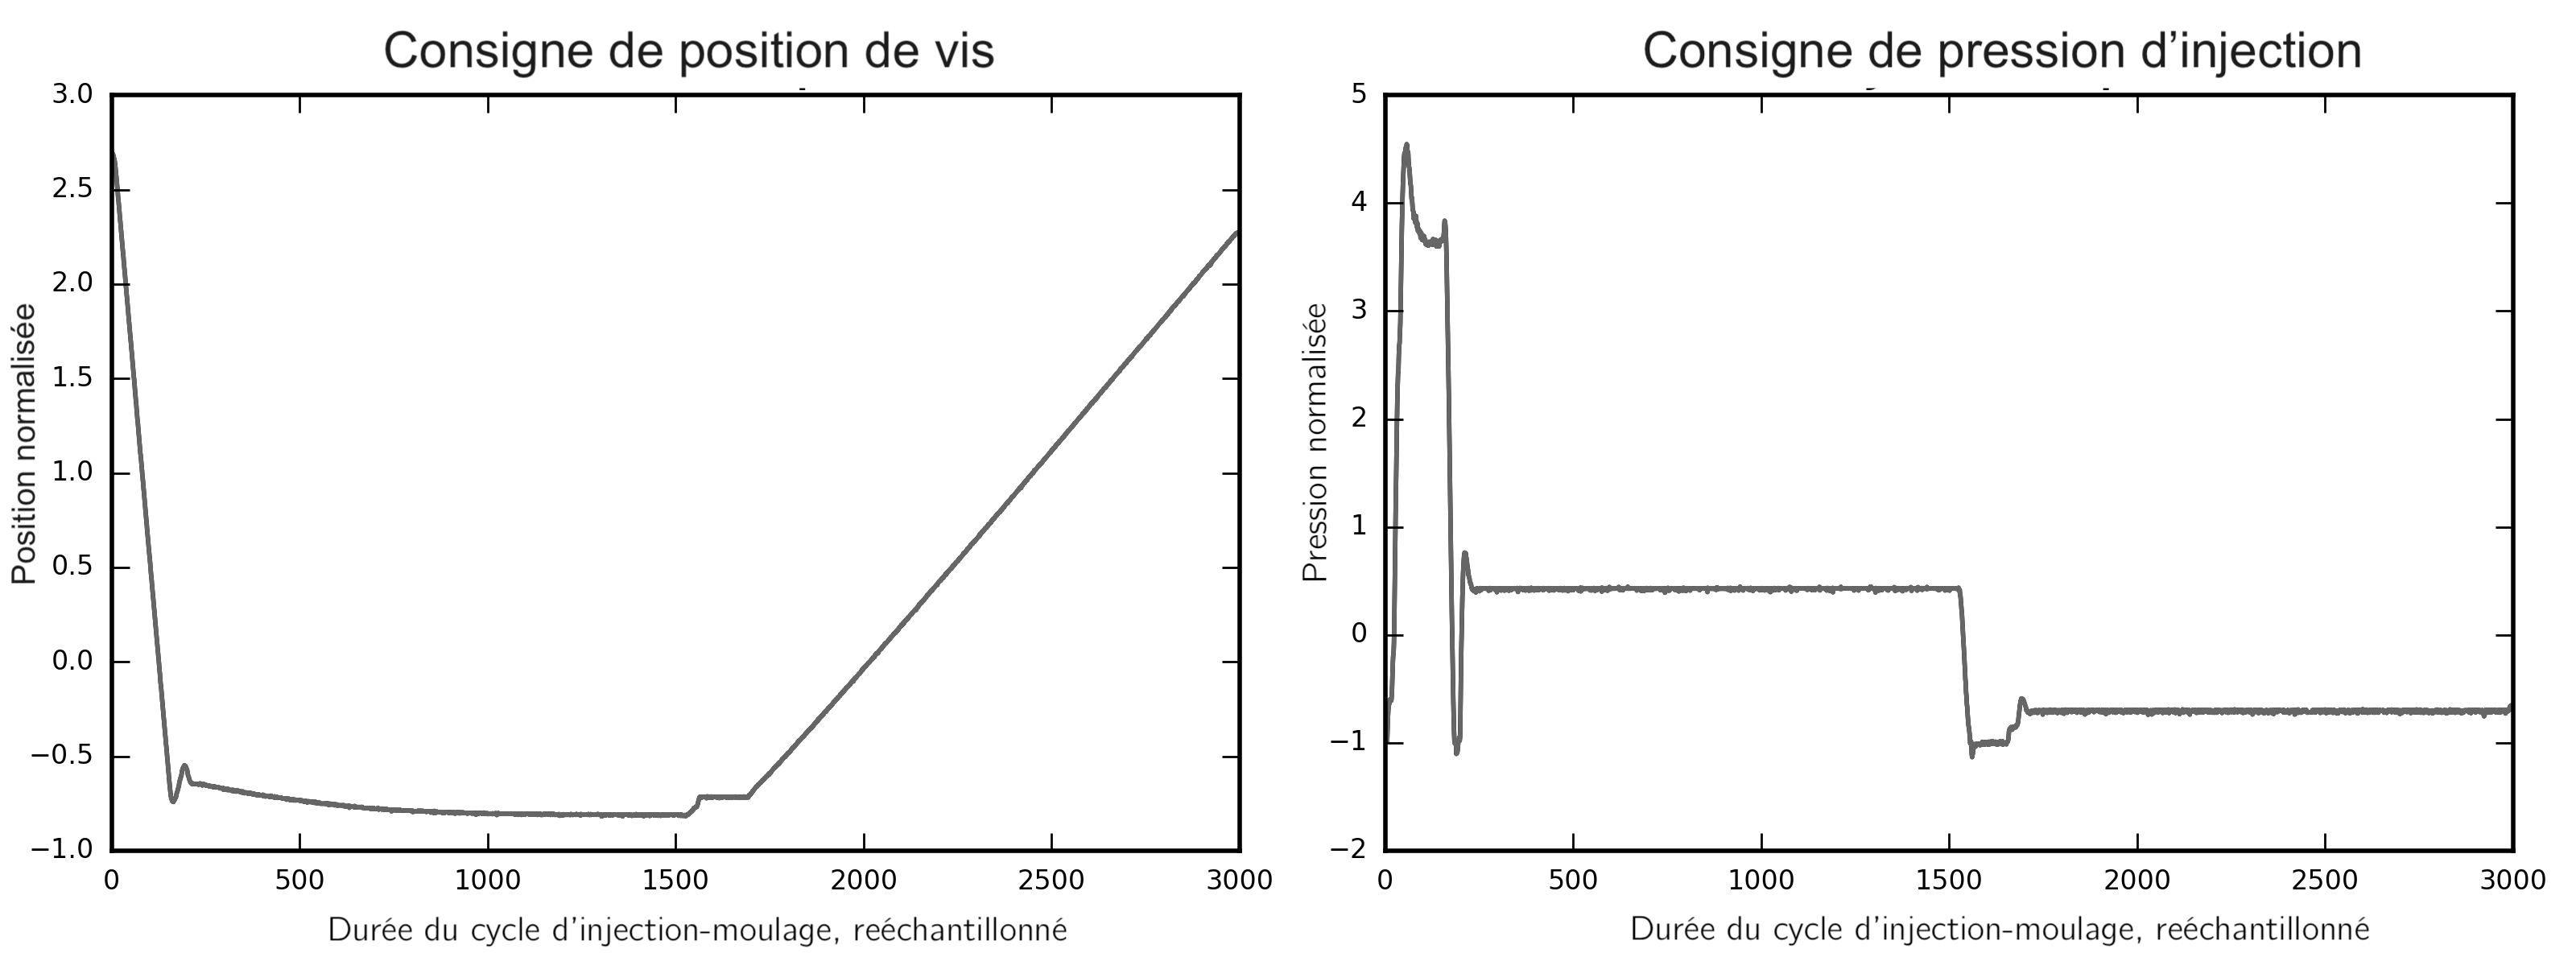
\includegraphics[width=\textwidth,height=\textheight,keepaspectratio]{../Chap1/Figures/part1_std_signals.png}
	\caption{Profil de position de la vis et de pression d'injection pendant un cycle d'injection-moulage.}
	\label{fig:molding_control}
\end{figure}

Des profils d'avance de la vis et de pression d'injection sont représentés dans la Figure \ref{fig:molding_control}.
On observe dans la première phase du cycke d'injection une avance rapide de la position de la vis et une augmentation de la pression d'injection, afin de remplir l'empreinte de matière fondue.
Une seconde phase est le maintien de la pression dans l'empreinte pendant le refroidissement de la matière.
Puis le moule est ouvert et la vis est progressivement reculé à sa position initiale.

La pratique industrielle utilise le savoir-faire du technicien régleur.  % pour régler le point de fonctionnement initial.
Le régleur a souvent accès à la courbe de pression de l'injection.
Sur des pièces compliquées, le réglage du procédé peut prendre plusieurs heures.

\bigskip

\bigskip

\begin{table}[thbp]
	\centering
	\arrayrulecolor{black}
	\hspace*{-14mm}
	\begin{tabular}{|llll|}
		\arrayrulecolor{black}
		%\cline{1-1} \cline{3-6}
		\hhline{----}
		Phase du procédé & Paramètres réglables & Description & Valeur classique \\ \hhline{=:=:=:=:} %\hline
		Dosage                   & Course de dosage                 & Distance de recul de la vis                                                    & 50-100 cm                      \\
		Dosage                   & Température du fourreau          & Températures des colliers chauffants                                   & 200-300 °C                     \\
		Dosage                   & Vitesse de rotation de la vis    & Rotation de la vis qui malaxe la matière                                                      & 1-20 tours/min                 \\
		Injection                & Course d'injection               & Distance d'avance de la vis pendant l'injection                                               & 50-100 cm                      \\
		Injection                & Pression d'injection             & Profil de pression exercée sur la vis et matière                            & 10-200 MPa                     \\
		Injection                & Pression de commutation          & Détermine le passage de l'injection au maintien & 10-100 MPa                     \\
		Injection                & Vitesse d'injection              & Vitesse d'avance de la vis                                                & 0,5 - 1 m/s                    \\
		Maintien-refroid. & Durée de maintien                & Durée de maintien de la pression                                                & 10-60 s                        \\
		Maintien-refroid. & Pression de maintien             & Profil de pression exercée sur la vis                            & 10-100 MPa                     \\
		Maintien-refroid. & Débit thermorégulateur           & Débit de circulation du fluide                    & 20-100 dm$^3$/s \\
		Maintien-refroid. & Température thermorégulateur     & Régulation thermique du moule                           & 10-40 °C                       \\
		Ouverture-éjection     & Course d'ouverture               & Distance d'ouverture de l'outillage                                       & 10-100 cm                      \\
		Ouverture-éjection     & Vitesse d'ouverture              & Vitesse d'ouverture de l'outillage                                        & 0,5 - 2 m/s                    \\
		Ouverture-éjection     & Course des éjecteurs             & Distance de sortie des éjecteurs                                      & 1-20 cm                        \\
		Ouverture-éjection     & Vitesse de rentrée des éjecteurs & Vitesse de sortie des éjecteurs                                                               & 0,5 - 2 m/s                    \\
		Fermeture outillage      & Vitesse de fermeture             & Vitesse de fermeture de l'outillage                                                           & 0,5 - 2 m/s                   \\
		\hline
	\end{tabular}%
	\caption{Paramètres réglables sur une presse à injecter classique.}
	\label{tab:process_parameters}
\end{table}


\newpage
\section{La qualité d'un produit en injection-moulage des thermoplastiques} \label{sec:quality_definition}

La norme ISO9000 \cite{ISO_9000_2015} spécifie la notion de qualité comme l'\textit{aptitude d'un ensemble de caractéristiques intrinsèques d'un objet à satisfaire des exigences}.
Dans notre cadre des produits industriels, les exigences sont celles du client final ou du donneur d'ordre.
Elles sont spécifiées dans la documentation technique du produit, dont le dessin.
Des caractéristiques sont mesurées sur le produit.
Puis les résultats sont comparées aux exigences, c'est à dire des limites d'acceptation ou des intervalles de tolérances.
Nous distinguons cinq grands types de caractéristique :
\begin{itemize}
	\item géométriques  % : normes ISO GPS \textit{Geometrical Product Specifications} \cite{ISO_8015_2011},
	\item mécaniques,
	\item sensoriels : visuelles, haptiques, olfactives,
	\item chimiques,
	\item économiques.
\end{itemize}

%Les pièces industrielles sur lesquelles nous avons travaillées sont fabriquées par injection-moulage de thermoplastiques.
%Dans le cadre de ce procédé, les caractéristiques chimiques sont définies par le choix de la matière initiale.
%Les caractéristiques économiques sont les coûts associés à la production des pièces.
%Les caractéristiques mécaniques dépendent du choix du matériau, de la géométrie des pièces et des paramètres du procédé d'injection-moulage.

Dans le cadre de ce travail, nous nous intéressons en particulier aux caractéristiques géométriques et d'aspect.
La maîtrise de ces deux types de caractéristique est un enjeu important pour le secteur de la plasturgie.
Les tolérances dimensionnelles sont de plus en plus serrées.
À celles-ci s'ajoutent l'exigence de peu de non-conformité de l'aspect des pièces.
Enfin, l'amélioration de la qualité est un facteur important de rentabilité et de compétitivité des entreprises.
Dès 1950, \citeauthor{deming_quality_1982} \cite{deming_quality_1982} décrit la réaction en chaîne que permet d'initier l'amélioration de la qualité : réduction des coûts des rebuts, diminution du prix de revient, gain de marchés et, à terme, création d'emplois.

Le Tableau \ref{tab:visual_defect} présente les non-conformités d'aspect habituelles en injection-moulage des thermoplastiques.


\begin{table}[htbp]
	\arrayrulecolor{black}
	\hspace*{-1mm}
	\begin{tabular}{|l|l|l|}
		\arrayrulecolor{black}
		\hline
		Non-conformité & Description & Causes probables \\ \hline \hline
		% Dimensionnelle & dimension non-conforme & température du moule, rigidité du moule, retassure \\ \hline \hline
		Homothétie & dimension modifiée & retrait de la matière \\ \hline
		Gauchissement & défaut de surface & refroidissement non homogène \\ \hline
		Retassure  & cavité dans la matière & pression de maintien, vitesse d'injection \\ \hline
		Incomplet & trou dans la pièce & quantité de matière injectée, clapet anti-retour défaillant \\ \hline
		Ligne de soudure & ligne décolorée &  pression d'injection, température matière \\ \hline
		Jet libre & trace décolorée & viscosité matière, conception moule, pression d'injection \\ \hline
		Éjection & trace de l'éjecteur & vitesse éjecteur, température matière, durée refroidissement \\ \hline \hline
		Combustion & trace noire & conception du moule, température de la matière \\ \hline
		Givrage & bulle ou trace blanche & matière humide \\ \hline
		Pollution & trace colorée & usure de l'outillage, pollution de la matière \\ \hline
	\end{tabular}
	\caption{Principaux défauts d'aspects en injection-moulage des thermoplastiques.}
	\label{tab:visual_defect}
\end{table}

% Sur des pièces qui seront utilisées en contraintes et en fatigues
Un défaut de ligne de soudure entraine une fragilité.
La majorité des non-conformités d'aspect sont des défauts géométriques de surface.
Seules la combustion, le givrage et la pollution sont entrainées pas la modification des propriétés du polymère.
Ces imperfections géométriques sont souvent dues au mauvais maintien du polymère contre les parois de l'outillage, ou bien à la solidification trop rapide de la matière.
Les défauts d'incomplets sont les plus simples à détecter par analyse d'image : un seuillage puis une détection de contours est suffisant.
La détection des autres non-conformité est plus compliquée.
C'est notre objectif principal de recherche.

La Figure \ref{fig:confocal_defect} présente une mesure par microscopie confocale d'un défaut de retassure sur une pièce plastique automobile de deux mètres.
Ce défaut est caractéristique des pièces automobiles qui sont peintes afin de réfléchir la lumière de manière harmonieuse.
La légère inflexion de la surface entraine une "cassure" de la réflexion de la lumière, ce qui attire le regard et amplifie l'impression de défaut.
L'écart géométrique de l'inflexion est de l'ordre de la dizaine de micromètres.

\bigskip

\begin{figure}[tbhp]
	\centering
	\begin{subfigure}[c]{0.48\textwidth}
		\centering
		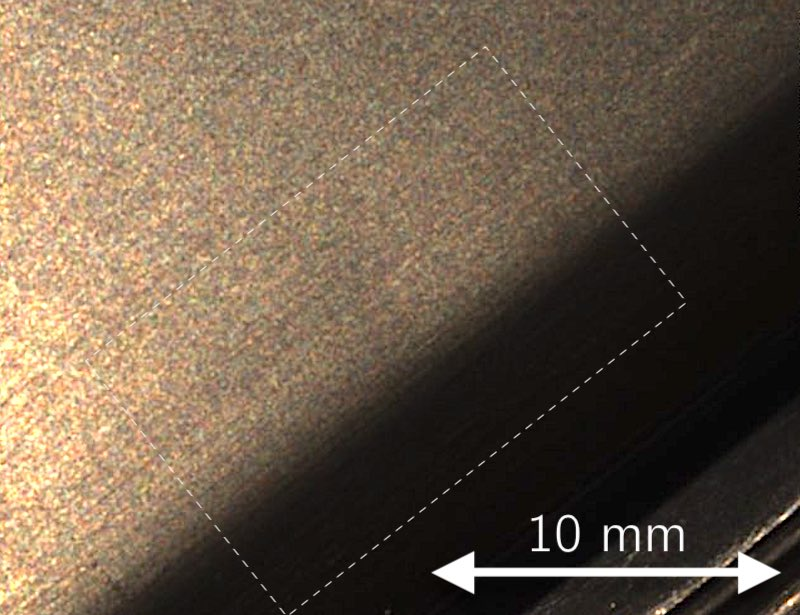
\includegraphics[width=\textwidth]{../Chap2/Figures/Cam1_Image_22_PO_defect_AVEC.jpg}
		\caption{Photographie du défaut.}
	\end{subfigure}
	\begin{subfigure}[c]{0.48\textwidth}
		\centering
		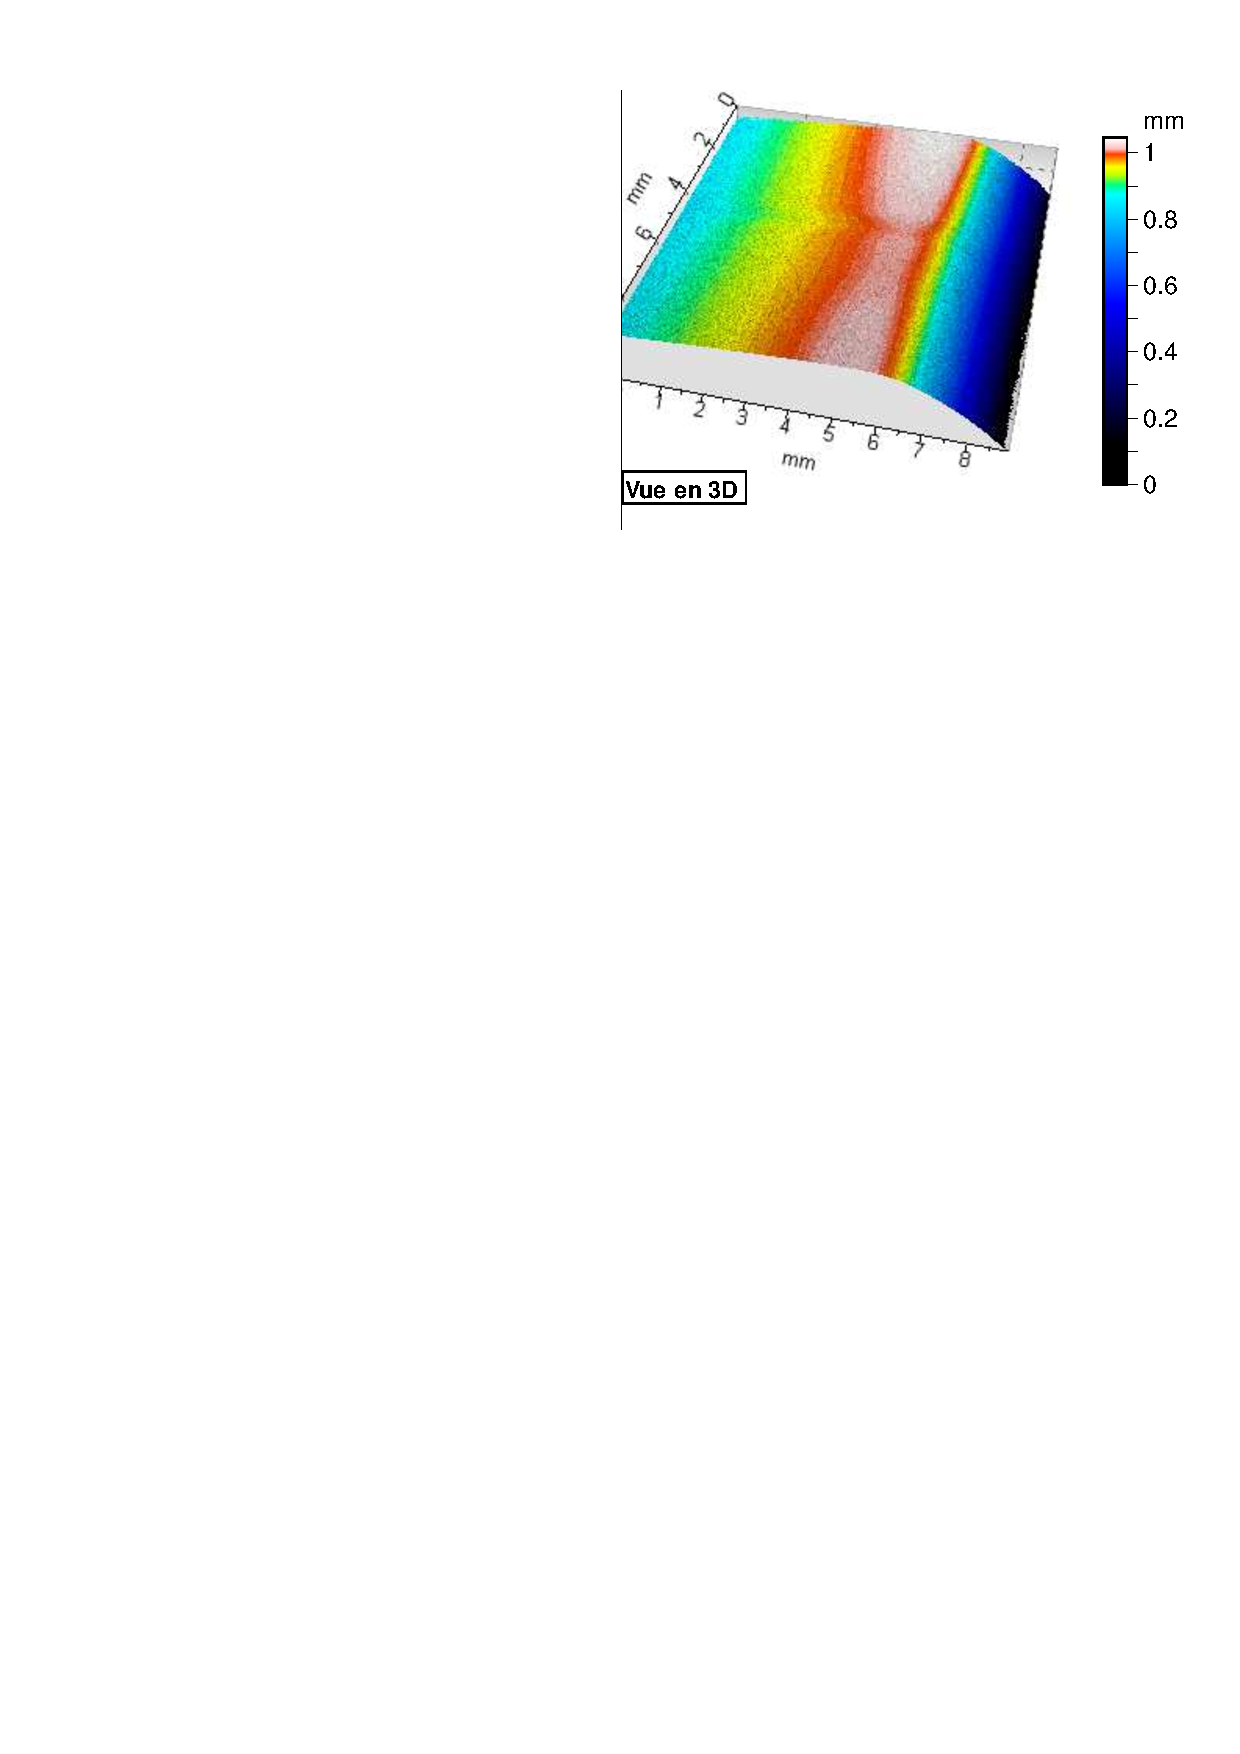
\includegraphics[width=\textwidth]{../Chap2/Figures/altisurf_defect.pdf}
		\caption{Mesure de surface par microscopie confocal.}
	\end{subfigure} \\
	\vspace{3\baselineskip}
	\begin{subfigure}[c]{\textwidth}
		\centering
		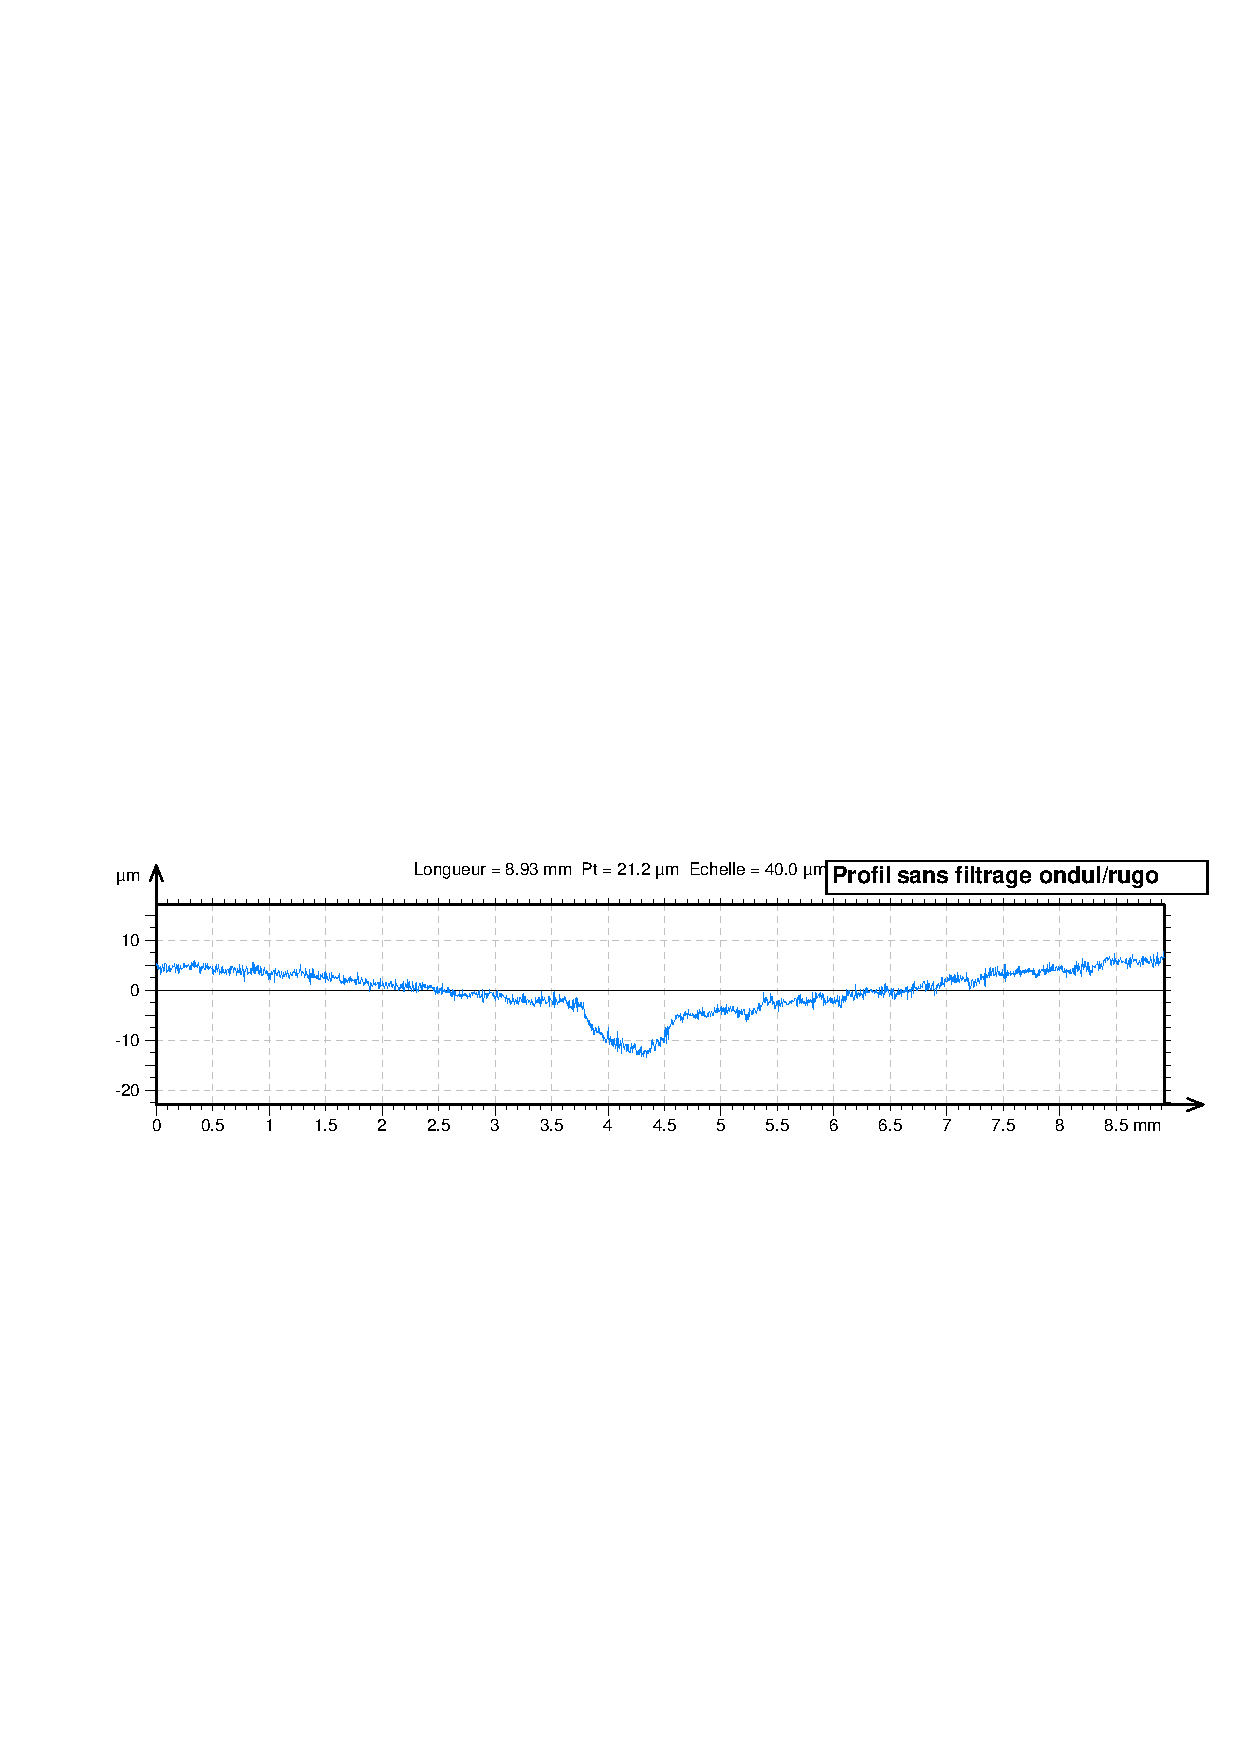
\includegraphics[width=\textwidth]{../Chap2/Figures/altisurf_defect_profil.pdf}
		\caption{Profil du défaut.}
	\end{subfigure}%  \hspace{20mm}%
	\caption{Défaut de retassure mesurée par microscope confocal, \textit{AltiMet 520} $^0$.}
	\label{fig:confocal_defect}
\end{figure}
% \footnotemark
\footnotetext{\href{https://www.altimet.fr/?page_id=236}{Spécifications techniques} de l'Altisurf 520 sur le site Internet de la société Altimet.}

\bigskip

La mesure de la géométrie à l'échelle micrométrique, pendant la durée du cycle du procédé, est un véritable défi.
Dans la suite de ce chapitre, nous présenterons les moyens de mesure existants ; puis nous orienterons notre étude sur les moyens de mesure sans contact ; en particulier nous nous intéresserons aux moyens de mesure compatibles avec le temps de cycle du procédé d'injection-moulage.


\newpage
\section{Revue de la recherche académique sur le procédé d'injection-moulage}  \label{sec:research_topics}
% Le projet de recherche collaboratif FUI SAPRISTI a pour objectif de limiter la production de pièces non-conformes.
Le procédé d'injection est l'étape clé du processus de fabrication des pièces plastiques moulées.
Il répercute ses défauts sur l'aval de la chaîne de production, comme par exemple sur les étapes d'assemblages et de finitions.

Dans cette section, nous identifierons trois axes de recherche principaux qui lui ont été dévoués : la modélisation physique du procédé ; la maîtrise du point de fonctionnement ; et l'optimisation des réglages.
Nous réaliserons une cartographie bibliographique §\ref{subsec:injection_research}, puis nous nous intéresserons aux travaux de modélisation du procédé d'injection-moulage §\ref{subsec:molding_model}.
Enfin, nous étudierons la recherche sur la maîtrise du procédé d'injection-moulage §\ref{subsec:process_control}.
% Enfin, nous discuterons de l'intérêt de notre travail sur le contrôle de la qualité en ligne, dans une perspective de surveillance et de pilotage du procédé.

\subsection{Cartographie bibliographique} \label{subsec:injection_research}
Afin d'identifier les thématiques de recherche qui sont associées au procédé d'injection-moulage, nous avons réalisé une cartographie bibliographique dans la Figure \ref{fig:cartographie}.
% \subsection{Revue bibliographique sur le procédé d'injection-moulage des thermoplastiques}
% Dans cette section, nous identifierons les principaux axes de recherche qui lui sont associés : la modélisation mathématique du procédé, la maîtrise du point de fonctionnement et l'optimisation des réglages.

\begin{figure}[bhtp]
	\centering
	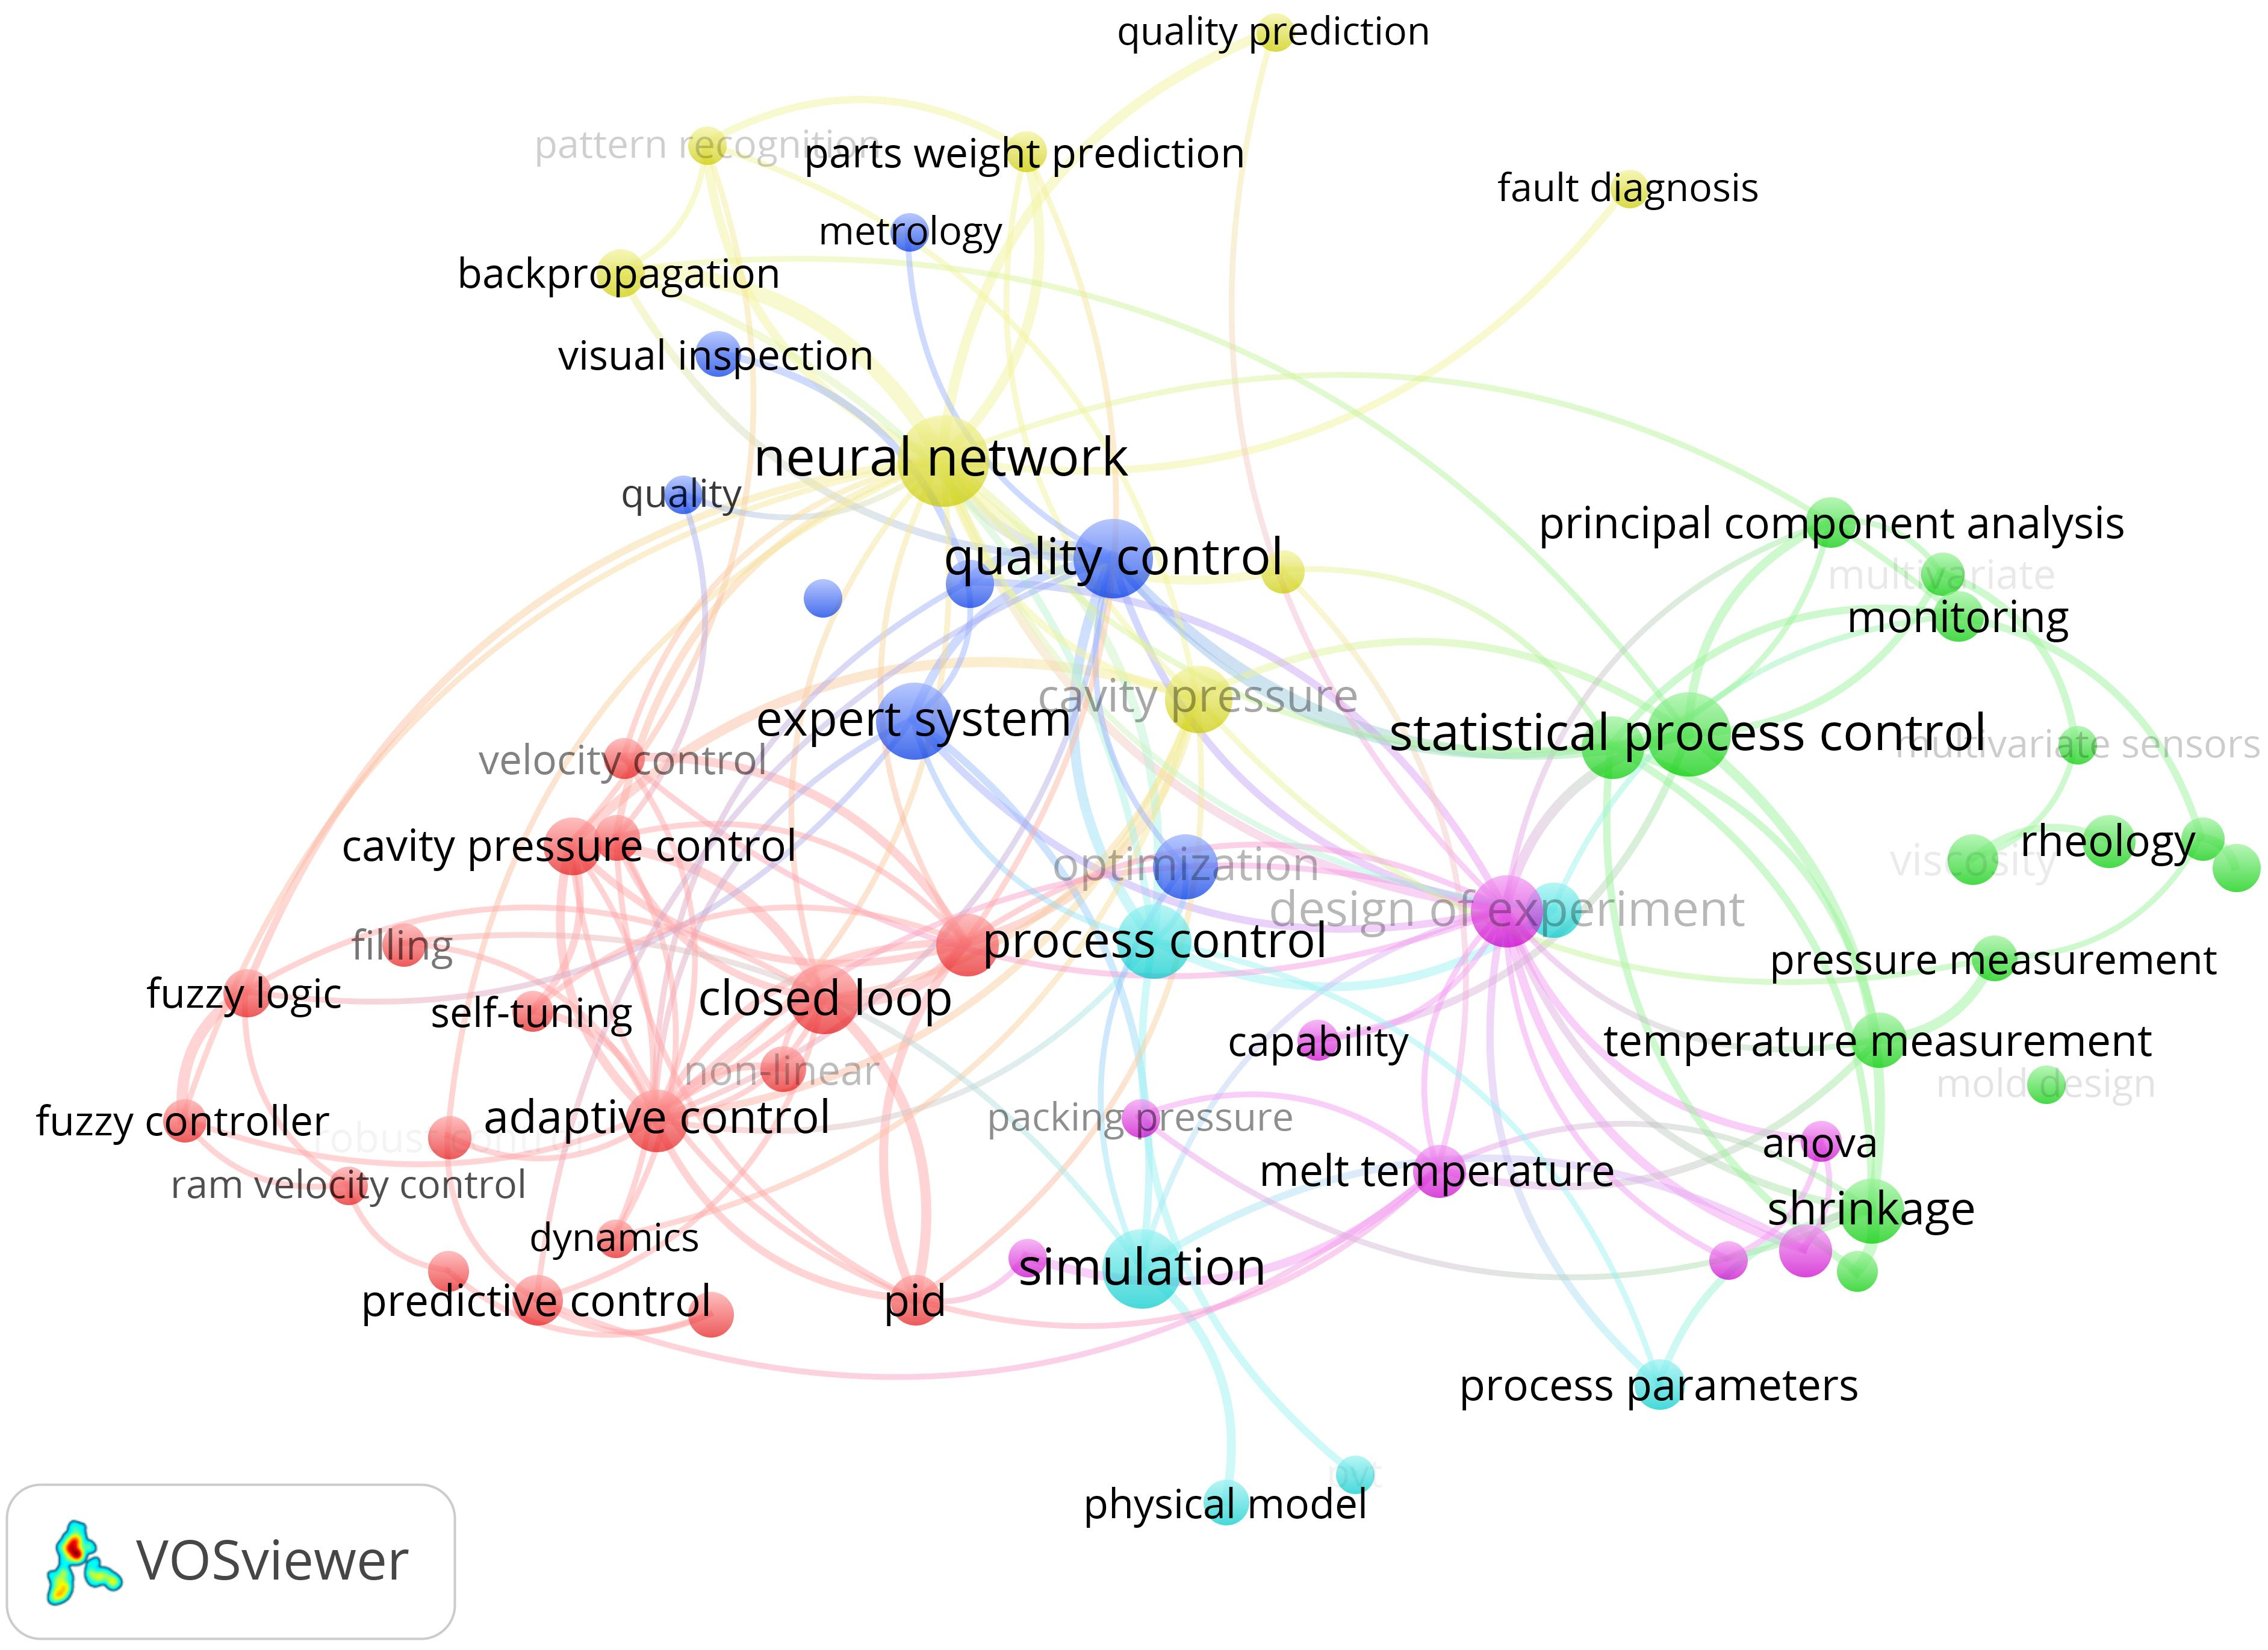
\includegraphics[width=\textwidth,height=\textheight,keepaspectratio]{../Chap1/Figures/tagMapFinalPubliOccurence.jpg}
	\caption{Cartographie bibliographique de la maîtrise du procédé d'injection-moulage.}
	\label{fig:cartographie}
\end{figure}

Elle présente le graphe relationnel que nous avons construit à partir des mots-clés associés à 421 publications, de 1970 à 2015.
Les mots-clés sont retenus s’ils apparaissent plus de quatre fois.
Ils sont regroupés par relations.
Nous utilisons le formalisme \textit{VOS} (\textit{Visualization Of Similarities}) proposé par \citeauthor{vaneck_vos_2006} \cite{vaneck_vos_2006, van_eck_comparison_2010}.
Sur ce graphique, nous identifions plusieurs thématiques de recherche.
Dans la suite de cette section, nous présenterons chacune d'elles.

\begin{itemize}
	\item la modélisation mathématique et la simulation du procédé (couleur cyan) §\ref{subsubsec:molding_theory},
	\item la modélisation empirique par plan d'expériences (couleur magenta) §\ref{parag:molding_doe},
	\item l’apport des systèmes à réseaux des neurones pour modéliser le procédé (en jaune) §\ref{parag:molding_neural},
	\item l’apport des systèmes experts pour régler le point de fonctionnement initial (en bleu) §\ref{subsec:process_control},
	\item la régulation du point de fonctionnement par l'automatique (couleur rouge, \textit{Engineering Process Control}) §\ref{subsec:process_control},
	\item l’analyse statistique afin de détecter les dérives (en vert, \textit{Statistical Process Control}) §\ref{subsec:process_control}.
\end{itemize}

% Dans la littérature, les réseaux de neurones sont utilisés pour modéliser le procédé de manière empirique.
% La littérature propose de réguler les paramètres du procédé d’injection à partir de la prédiction de caractéristiques des pièces.
% La prédiction à partir de variables du procédé est préférée à une mesure directe sur la pièce, car la métrologie n’est pas assez développée pour permettre une mesure pièce à pièce en cycle industriel.
% À contrario, l'enregistrement des mesures de pression pendant le cycle est très répandue, car elle est implémentée par les fabricants de moules et les fabricants de systèmes de régulations du procédé.
% Enfin, nous distinguons (de couleur rouge) les efforts pour la régulation du procédé.
% De nombreuses méthodes ont été étudiées et nous remarquons l’intérêt porté aux méthodes adaptatives.
% Cependant, chacune de ces méthodes ne s’intéressent qu’à un nombre limité de variables du procédé et des caractéristiques du produit.
% Enfin, l'analyse statistique est utilisée pour détecter les dérives et les défaillances du procédé.
% Elle s’appuie sur la mesure \textit{in-situ} de variables du procédé, parmi lesquelles les plus utilisées sont la température et la pression.
% Ce graphique n'inclut pas les dates des publications.
% Nous invitons le lecteur à consulter notre Tableau récapitulatif \ref{tab:state_art_compare}.
\noindent
L'ensemble de ces travaux de recherche a deux grands objectifs :
\begin{itemize}
	\item améliorer la modélisation du procédé pour pouvoir optimiser ses paramètres,
	\item maîtriser les caractéristiques des produits fabriqués.
\end{itemize}
Ces deux objectifs sont souvent traités de manière complémentaire.
% L'amélioration de la modélisation permet une meilleur maîtrise des caractéristiques du produit.
Dans les sections suivantes, nous présenterons chacune de ces thématiques de recherche.

\subsection{Modélisation du procédé d'injection-moulage} \label{subsec:molding_model}
% Le moulage par injection-plastique est un procédé séquentiel amdécomposé en plusieurs phases interdépendantes.
Chacune des phases du procédé d'injection-moulage influe sur la suivante et, à terme, conditionne les caractéristiques du produit.
Nous étudierons les travaux de la littérature sur la modélisation systémique du procédé, puis nous proposerons une nouvelle représentation systémique.
Nous présenterons ensuite les travaux sur les modèles théoriques du procédé d'injection-moulage et les travaux d'identification de modèles à partir de résultats de mesure expérimentaux.

\subsubsection{Modélisation systémique} \label{subsubsec:molding_systemic}
En 1999, \citeauthor{kazmer_towards_1999} proposent un découpage en cinq phases \cite{kazmer_towards_1999} (voir la Figure \ref{fig:kazmer_systematic}) qui est une évolution du découpage en trois phases qui avait été proposé par \citeauthor{ma_design_1974} \cite{ma_design_1974}.
Cette représentation systémique du procédé fait apparaître des variables d’état intermédiaires qui sont associées à chacune des phases.

\begin{figure}[bthp]
	\centering
	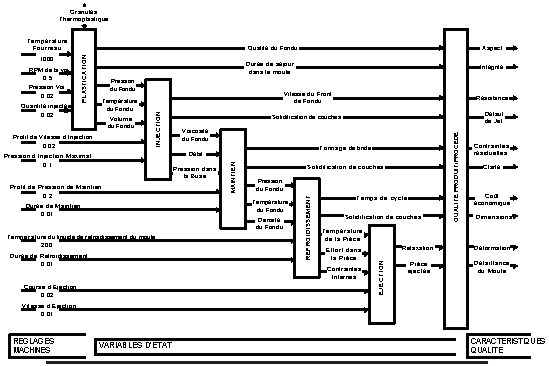
\includegraphics[width=\textwidth,height=\textheight,keepaspectratio]{../Chap1/Figures/Kazmer_1999-Process.pdf}
	\caption[Vue systémique du procédé d'injection-moulage.]{Vue systémique du procédé d'injection-moulage, traduite de \citeauthor{kazmer_towards_1999} \cite{kazmer_towards_1999}.}
	\label{fig:kazmer_systematic}
\end{figure}

Elle fait également apparaître les relations de dépendance entre les différentes phases.
% Les phases sont la cause des caractéristiques du produit.
La représentation met en évidence plusieurs variables intermédiaires, qui influent soit directement sur les caractéristiques du produit, soit sur les caractéristiques d'autres phases.
Ces variables intermédiaires ne sont pas nécessairement observables.
Il est par exemple très difficile de mesurer la densité de la matière fondue, ou encore l'évolution des contraintes internes.

Cette figure permet de mettre en évidence dix caractéristiques du produit qui sont la cause de 12 variables de réglage.
L'injection-moulage est un procédé multi-entrées, multi-sorties (MIMO).
On distingue également deux réglages de "profils".
Un profil est une valeur de réglage qui évolue dans le temps.
Aussi, les possibilités de réglages d'un profil sont bien plus importantes que pour une grandeur scalaire. Dans le cas où un profil serait représenté par 10 points ; nous obtenons alors 20 variables de réglage pour deux profils.
% La modélisation d'un tel procédé est compliquée.
% C'est pourquoi la littérature est riche en modèles empiriques, car les modèles théoriques sont difficiles à réaliser.

%\begin{figure}[bthp]
%	\centering
%	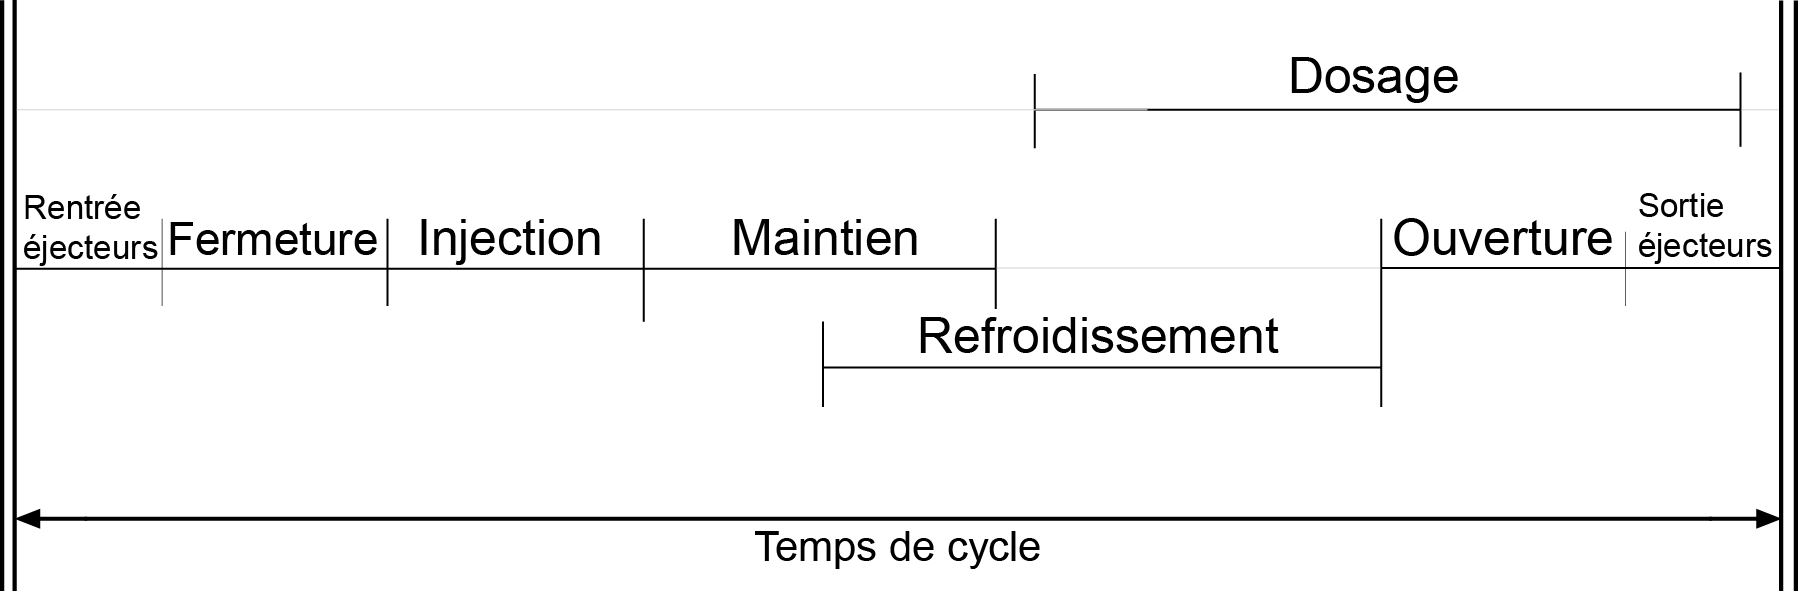
\includegraphics[width=0.82\textwidth,height=\textheight,keepaspectratio]{../Chap1/Figures/SAPRISTI_Chronogramme-Simple.png}
%	\caption{Chronogramme du cycle d'injection-moulage.}
%	\label{fig:chronogramme}
%\end{figure}

Enfin, nous remarquons que cette représentation systémique ne fait pas apparaître la nature cyclique du procédé.
% C'est pourquoi nous proposons un chronogramme du cycle d’injection : la Figure \ref{fig:chronogramme} représente le caractère cyclique du procédé, en particulier pour l'étape de dosage.
En effet, la phase de dosage est réalisée en temps masqué au cycle principal de fabrication d'une pièce.

\begin{figure}[hbtp]
	\centering
	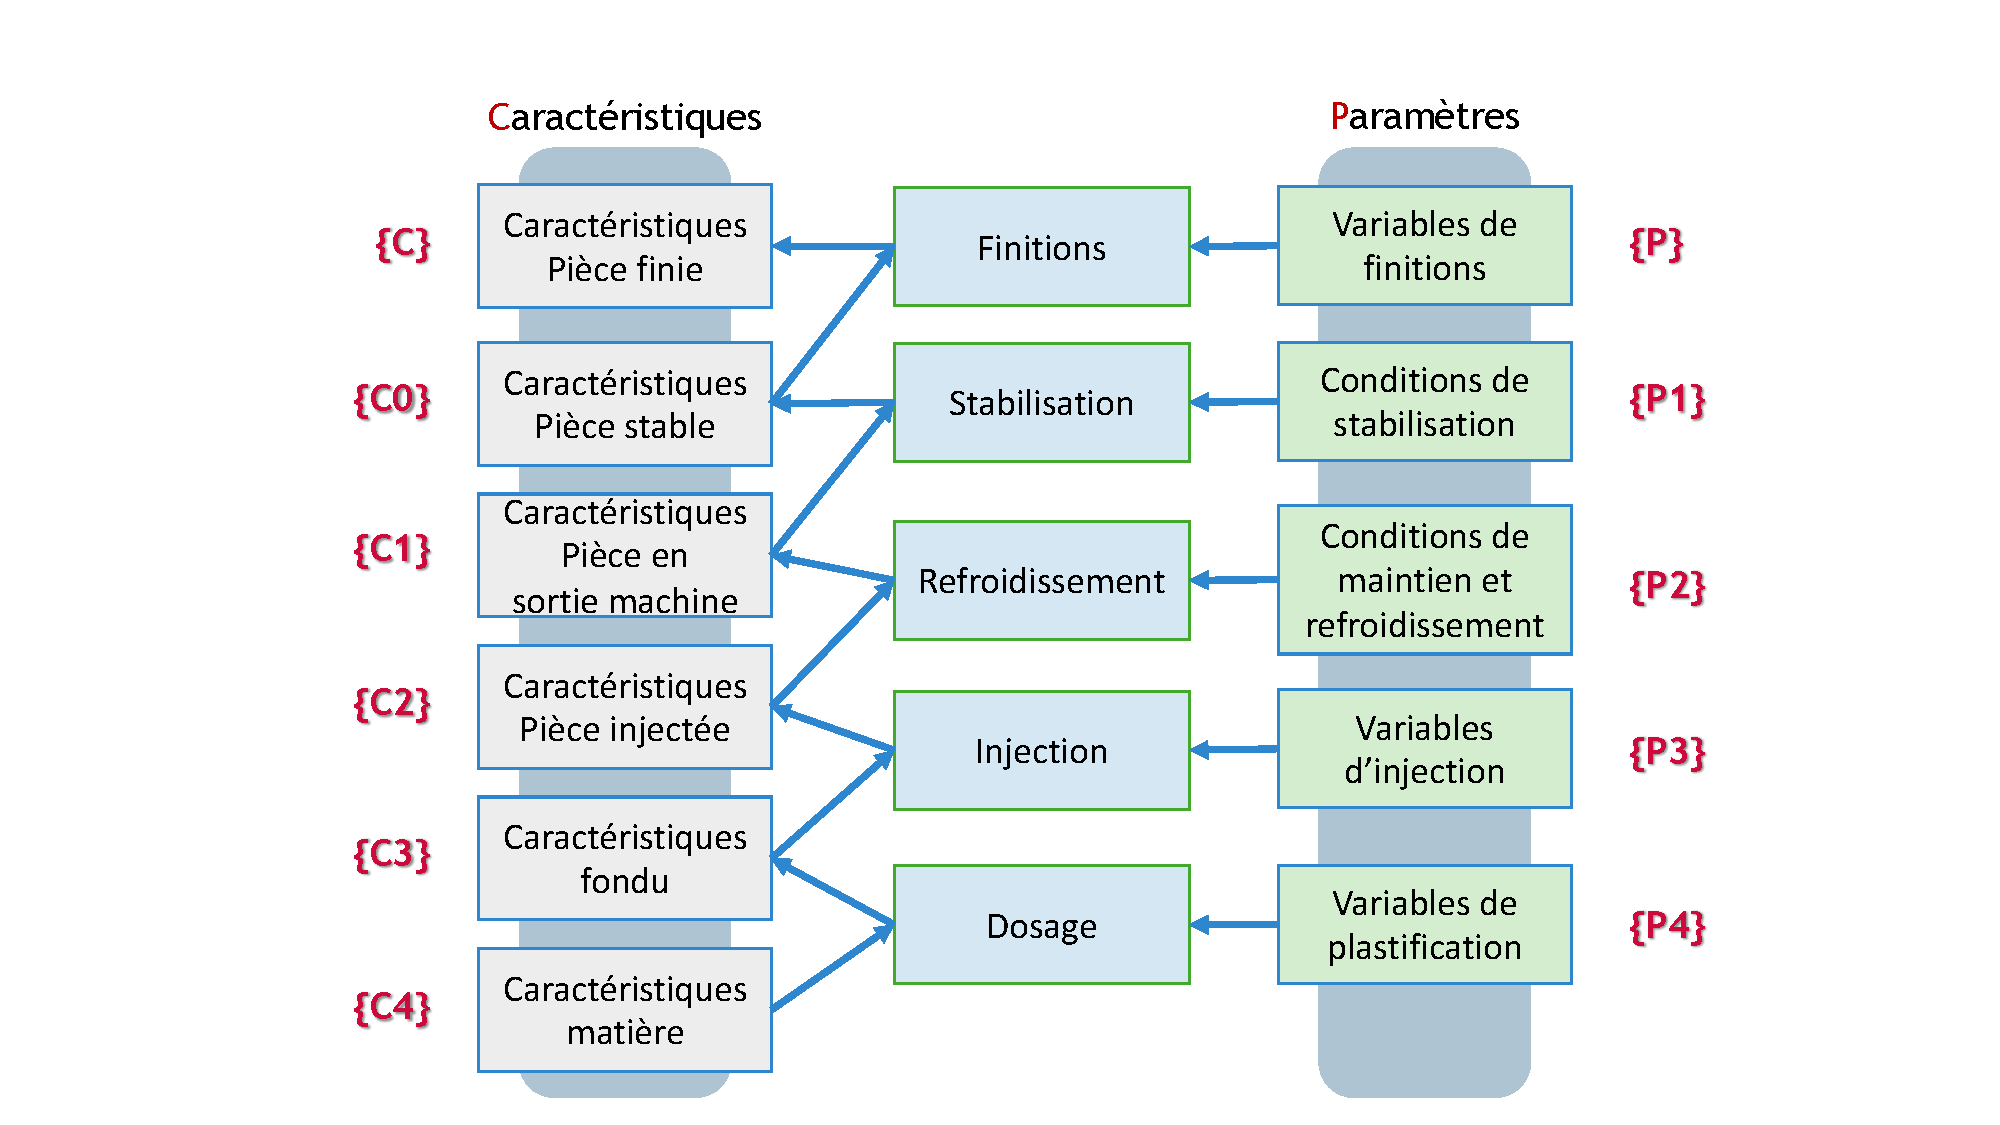
\includegraphics[width=0.85\textwidth,height=\textheight,keepaspectratio]{../Chap1/Figures/Sapristi_ZigZag.pdf}
	\caption{Représentation \textit{Zig Zag} du procédé d'injection-moulage des thermoplastiques.}
	\label{fig:zigzag}
\end{figure}

Nous nous appuyons sur la méthodologie \textit{Axiomatic Design} pour représenter le procédé \cite{suh_principles_1990}.
\citeauthor{suh_principles_1990} propose la représentation \textit{Zig Zag}, afin de mettre en évidence les liens entre les paramètres d'un procédé (\textit{Process Variables}) et les caractéristiques d'un produit (\textit{Design Parameters}).
Dans la Figure \ref{fig:zigzag}, nous proposons une représentation \textit{Zig Zag} du procédé d'injection-moulage.
% À la différence de la vue systémique de la Figure \ref{fig:kazmer_systematic},
La représentation \textit{Zig Zag} fait apparaître les variables du procédé $\boldsymbol{P_i}$ et les caractéristiques du produit lors de chacune des phases $\boldsymbol{C_i}$.
Les caractéristiques du produit fini $\boldsymbol{C}$ sont fonction de l’ensemble des phases.
De plus, chaque phase est fonction des phases précédentes, ainsi que des variables du procédé.
Si un réglage est modifié au niveau de l’une des phases $i$, les caractéristiques du procédé pour toutes les phases suivantes $\boldsymbol{C_{j>i}}$ pourront être modifiées.
% Dans la suite de notre étude du procédé d'injection-moulage, nous indiquerons à quelle phase de notre représentation correspond les différents travaux cités.

Nous remarquons en particulier que les caractéristiques d'une pièce finie sont liées aux phases de stabilisation et de finition.
Or, la stabilisation de pièces prend du temps.
Sur des pièces massives, il faut attendre plusieurs heures que la pièce refroidisse et que les contraintes internes se stabilisent.
C'est pourquoi, les étapes de finition sont généralement réalisées plusieurs heures après l'injection-moulage d'une pièce.

Dans la suite de cette section, nous présenterons les publications les plus importantes concernant la modélisation du procédé d'injection-moulage.
Nous distinguons les modélisations physiques, qui cherchent à proposer un modèle mathématique du procédé à partir de connaissances théoriques, des modélisations empiriques qui utilisent les données d'expériences pour identifier un modèle mathématique.


\subsubsection{Modélisations physiques du procédé d'injection-moulage} \label{subsubsec:molding_theory}
La nature multivariée du procédé rend difficile la définition d'un modèle théorique.
En 1987, \citeauthor{agrawal_injection-molding_1987} estiment, en conclusion de leur revue de la régulation du procédé d'injection-moulage, que les futurs travaux de recherche devront prendre en compte l’ensemble des variables d'entrée, ainsi que leurs interactions \cite{agrawal_injection-molding_1987}.
Pourtant, d'après le Tableau \ref{tab:state_art_compare} aucun des modèles proposés dans la littérature après 1987 ne prend en compte l'ensemble des 12 variables de ce procédé, telles que présentées dans la Figure \ref{fig:kazmer_systematic}, voir l'Annexe \ref{Ann:process_control} Tableau \ref{tab:state_art_compare}.

Un modèle théorique doit prendre en compte les nombreuses interactions multi-physiques entre chaque phase du procédé.
De plus, la connaissance de la physique des polymères reste un champ de recherche ouvert.
L'évolution de la cristallinité d'un polymère, lors de sa solidification, peut par exemple être modélisée par l'équation de \citeauthor{nakamura_aspects_1972} \cite{nakamura_aspects_1972, nakamura_aspects_1973}.
Le lecteur intéressé la modélisation micro-mécanique des polymères semi-cristallin pourra se référer à la monographie de \citeauthor{galeski_nano_2009} \cite{galeski_nano_2009}.
Les auteurs discutent en particulier des contraintes thermo-mécaniques qui s'exercent sur la matière pendant un cycle de production.
Ils analysent les conséquences de ces contraintes sur les propriétés cristallographiques et sur les propriétés mécaniques macroscopiques des pièces.
% The promotion of energy dissipative processes that delay or entirely suppress fracture processes originating from imperfections in the internal structure or scratches and notches is enhanced by cavitation. In almost all cases, cavitation either makes possible further toughening by activating other mechanisms or itself contributes to the plastic response of the polymer. The most energy dissipative processes, crazing and shear yielding, occur at a reduced stress level.
% In crystalline polymer systems the tough response, besides cavitation and crazing, is crystallographic in nature. Crystallographic slips are the main plastic deformation mechanisms that require generation and motion of crystallographic dislocations. The concepts of generation of monolithic and half-loop dislocations plausibly explain the observed yield stress dependences on crystal thickness, temperature and strain rate.
% It appeared that a successful modeling of mechanical properties of crystal- line polymers within the elastic range requires a consideration of lamellae thick- ness and crystallinity but also the lamellae width and length. Varying elastic properties of the amorphous phase are to be considered when the constraints between lamellar crystals change due to differentiated solidification conditions.

À l'échelle macroscopique, plusieurs travaux propose de modéliser les phases de dosage, injection, maintien et le refroidissement.
En 1991, \citeauthor{chiu_dynamic_1991} proposent un modèle non-linéaire des phases de dosage et d'injection, à partir des lois d'écoulement d'un fluide visqueux et compressible \cite{chiu_dynamic_1991}.
Huit variables d’état sont utilisées : délai avant le début du dosage, pression d’arrivée de la matière pour le dosage, pression d’injection, position de la vis, pression de la vis, volume du polymère dans l’empreinte et débit du polymère.
Leur travail compare le modèle avec des mesures de pression et de température dans l'outillage : les profils des résultats de mesure et du modèle sont similaires.
En 2004, \citeauthor{bereaux_series_2004} proposent un modèle de l'étape de dosage et de la plastification du polymère, à partir des lois d'écoulement non-newtoniennes des polymères visqueux \cite{bereaux_series_2004}.  % et d'évolution des caractéristiques de la matière
Les travaux de doctorat de \citeauthor{legoff_etude_2006} propose une modélisation des phases de maintien et de refroidissement, qui s'appuie sur les transferts thermiques au niveau des parois \cite{legoff_study_2005, legoff_etude_2006}.
En particulier, \citeauthor{legoff_etude_2006} montre qu'il est nécessaire de prendre en compte la transformation cristalline du polymère, car les propriétés thermiques de ce dernier évoluent pendant le refroidissement.
% Or une différence de plus de 20°C est cependant mesurée ($\boldsymbol{C_2, P_3}$).
% À partir d'une mesure invasive à l'aide d'un capteur de température positionné dans l'outillage, ce travail identifie un modèle qui prend en compte l'évolution du contact du point de vue des transferts thermiques.

Enfin, la méthode des éléments finis permet d'appliquer des modèles physiques élémentaires sur des millions d'éléments discrets.
Elle est particulièrement utilisée pour modéliser les phases de dosage et d'injection du polymère fondu \cite{moguedet_use_2009}.
À partir de la simulation de l'évolution des variables du procédé, elle permet également d’optimiser la conception des outillages et de dimensionner les structures \cite{gao_adaptive_2008}.
% Ces simulations sont coûteuses en ressources de calculs et en temps.
% Leurs utilisations pour ajuster les réglages nécessite que le résultat soit obtenu pendant la durée du temps de cycle du procédé.
% Malgré les puissances de calculs aujourd’hui disponibles, cette durée est toujours incompatible.
% Les simulations éléments-finis sont en revanche indispensables pour la conception des pièces et des outillages, car elles permettent le dimensionnement des structures.

L'ensemble de ces travaux s'intéressent à des phases spécifiques du procédé.
À notre connaissance, aucun travail de la littérature ne prend en compte l'ensemble des phases et des paramètres du procédé, telles que présentés dans la Figure \ref{fig:zigzag}.
Dans la suite de nos travaux, nous ne nous appuierons pas sur les connaissances de modèles physiques.
% Nous avons choisi d'utiliser une démarche empirique de recherche.
En effet, notre problématique de contrôle de la qualité nécessite de répondre à une grande variété de cas d'applications.
Cependant, les modèles théoriques de la littérature sont spécifiques à certains matériaux et à certains cas d'applications.
% Nous nous intéresserons en particulier à la modélisation des caractéristiques des pièces produites, pour des paramètres du procédé données.
De plus, les modèles théoriques aujourd'hui établis ne permettent pas de simuler l'ensemble des caractéristiques du produit que nous devons contrôler.
% En particulier, les caractéristiques d'aspect des pièces ne sont pas étudiées.

\subsubsection{Modélisations empiriques du procédé d'injection-moulage}
La littérature en injection-moulage est fournie d'études expérimentales.
La démarche classique est l'identification de modèles à partir de mesurages sur le procédé.
% Au travers de ces études, l'ensemble des paramètres du procédé a été étudié.
% Cependant, 
% Dans le cadre de notre travail, nous choisissons d'utiliser une démarche empirique pour étudier les caractéristiques du produit.
% Nous proposons une revue des travaux représentatif de l'évolution de cette thématique de recherche dans notre état de l'art \cite{nagorny_injection_2017}.

Dès 1974, \citeauthor{ma_design_1974} propose de modéliser les phases du procédé à l'aide de fonctions polynomiales, qui sont identifiées par des mesures expérimentales \cite{ma_design_1974}.
Il discute de l'utilisation du support informatique pour stocker les données, définir les fonctions et réaliser l'identification.
% La modélisation informatique des procédés a émergé avec le développement des micro-contrôleurs.
% Le modèle complet du procédé est une composé de l'ensemble des fonctions qui modélisent chaque phase.
La modélisation du procédé complet est la composé des modèles fonctionnels des différentes phases successives.
Ce travail ne propose pas de validation expérimentale de la méthode présentée.

En 2000, \citeauthor{delaunay_nature_2000} montrent l'influence de la déformation du moule pendant le cycle d'injection \cite{delaunay_nature_2000}.
Ce travail étudie les limites des modèles existants à partir de mesures expérimentales pendant les phases de maintien et de refroidissement.
Ils montrent également la nécessité de prendre en compte l'évolution du contact entre le polymère et les parois du moule \cite{delaunay_nature_2000a}.
En effet, la matière fondue n'est pas en contact continu avec la paroi.
Des poches d'airs peuvent se former ; ce qui modifie sensiblement les variables de refroidissement et la cristallisation du polymère.
Les travaux antérieurs assumaient que le moule était indéformable et que le contact entre le moule et le polymère était parfait.
La démarche de ces travaux est l'identification des paramètres d'un modèle polynomial, à partir de mesures de température et de pression dans le moule.
Les auteurs remarquent la nécessité de modéliser le couplage entre l'évolution de la géométrie du moule et le refroidissement, pour simuler correctement les contraintes imposées à la matière.
% Les limites de la modélisation mathématique du procédé d'injection-moulage sont les hypothèses fortes qui sont faites en amont.
% De plus, l'injection-moulage est un procédé multivarié.
% Il est alors nécessaire de prendre en compte l'ensemble des interactions entre les paramètres.
Les modèles identifiés par les auteurs sont limités aux cas d'études spécifiques sur lesquelles les mesures expérimentales ont été réalisées.

Nous remarquons, dans la littérature de l'injection-moulage, deux grandes démarches utilisées pour identifier des modèles multivariés :
\begin{itemize}
\item l'exploration et la modélisation du procédé par les plans d'expériences §\ref{parag:molding_doe} qui permet d'identifier des modèles empiriques,
\item l'identification de modèles par apprentissage, à l'aide de réseaux de neurones §\ref{parag:molding_neural}.
\end{itemize}

\paragraph{1.3.2.3.1 Plan d'expériences}\mbox{} \label{parag:molding_doe} \\
Les plans d’expériences permettent de construire un modèle polynomiale d’un système à plusieurs paramètres.
De plus, ils permettent d'adapter la quantité d’essais expérimentaux à réaliser en fonction de l'ordre du modèle que l'on cherche à obtenir.
Les essais sont réalisés suivant une table de variation des paramètres.
Nous discutons des plans d'expériences dans le Chapitre \ref{ch:dataset} Section \ref{subsec:doe}.
Le modèle obtenu permet théoriquement d'optimiser une sortie en fonction des paramètres, et ainsi, comme tout modèle de trouver un point de fonctionnement idéal.

En 1993, \citeauthor{regnier_local_1993} sont les premiers à proposer l'utilisation des plans d'expériences pour identifier un modèle polynomial d'ordre 2 avec interactions du phénomène de retrait, à partir de 6 paramètres du procédé \cite{regnier_local_1993, regnier_experimental_1994}.
De nombreux travaux utiliseront par la suite cette démarche expérimentale.
% En 1994, \citeauthor{blyskal_applying_1994} utilisent les plans d’expériences afin de déterminer les paramètres optimaux pour produire des dimensions de pièces cibles \cite{blyskal_applying_1994}.
En 2013, \citeauthor{fei_practical_2013} réalisent une étude rétrospective de 1999 à 2010, sur l’utilisation de la méthode des plans d'expériences en injection-moulage \cite{fei_practical_2013}.  % de Taguchi 
Ils distinguent deux utilisations faites dans la littérature :
\begin{itemize}
	\item produire un jeu de données expérimentales pour identifier des modèles,
	\item limiter le coût de l'optimisation par simulations numériques en utilisant un modèle intermédiaire construit par plans d'expériences.
\end{itemize}

L'étude de \citeauthor{fei_practical_2013} remarque en particulier qu'un nombre important de modèles est identifié par apprentissage, à l'aide de réseaux de neurones.
La théorie des plans d'expériences permet d'identifier des modèles polynomiaux.
Or, les variables qui entrent en jeu dans le procédé d'injection-moulage ont souvent des réponses non linéaires par rapport aux paramètres de réglages et des interactions qui peuvent être difficilement modélisé par des polynômes.
C'est pourquoi les modèles à réseaux de neurones ont été largement utilisés dans la littérature.

Nous utiliserons dans nos travaux un plan d'expériences de criblage pour construire notre jeu de données, dans le Chapitre \ref{ch:dataset}.
Cela permet de parcourir un espace représentatif de la plage de fonctionnement du procédé en un minimum d'essais.

\paragraph{1.3.2.3.2 Modélisation par réseaux de neurones}\mbox{} \label{parag:molding_neural} \\
L'utilisation des réseaux de neurones pour la modélisation dans les systèmes industriels est proposée dès 1980.
% Le procédé d'injection plastique possède des paramètres interdépendants et non-linéaires.
Un réseau de neurones est une composée de fonctions non-linéaires.
Il est adapté à l'identification de modèles aux multiples entrées.
Il est intéressant de noter que le procédé d'injection-moulage est également représenté par une composition de fonctions dans la littérature : \citeauthor{ma_design_1974} \cite{ma_design_1974} utilise une fonction polynômiale pour modéliser chaque phase du procédé.

% Dans le cadre de notre travail, nous utiliserons des réseaux de neurones pour modéliser la notion de qualité à partir des mesures sur les pièces.
% Nous détaillons les algorithmes à réseaux de neurones dans le Chapitre \ref{ch:metric_learning} §\ref{parag:neural_networks}.

En 2000, \citeauthor{schnerr-haselbarth_automation_2000} proposent le système \textit{Intelligent Quality Control} \cite{schnerr-haselbarth_automation_2000}.
Un algorithme à réseaux de neurones est utilisé pour prédire la caractéristique de la masse des pièces produites, à partir des variables du procédé.
Les données d’apprentissage proviennent d’un plan d'expériences factoriel à trois niveaux, sur trois paramètres du procédé : température du fondu, pression de maintien et vitesse d’injection.
À intervalle temporels régulier, 150 points de mesure de la pression dans le moule sont enregistrés pendant les phases d’injection et de maintien.
La masse de la pièce est mesurée dès la sortie de la machine avec une résolution au 1 milligramme ; les expériences conduisent à une variation de masse de 1,4\%.
Le réseau est alors capable de prédire la masse des pièces avec une exactitude de 86\%, soit une moyenne de 5 milligrammes d’erreur sur une masse total de 35 milligrammes.
Ces résultats mettent en valeur l'intérêt des modèles qui utilisent des réseaux de neurones.

\subsection{Maîtrise du procédé d'injection-moulage des thermoplastiques} \label{subsec:process_control}
Dans cette section, nous positionnerons notre travail de contrôle de la qualité en ligne de production dans la thématique de recherche de la maîtrise du procédé d'injection-moulage.
L'objectif final est de maîtriser la qualité du produit : c'est à dire de limiter la dispersion des caractéristiques des pièces produites.
% Il s'agit en priorité d'effectuer des mesures pertinentes sur l'état du procédé, puis de les analyser afin de détecter les dérives.
Nous résumons cette démarche en nous référant à notre représentation \textit{Zig-Zag} Figure \ref{fig:zigzag} :
\begin{enumerate}
	\item réglage initial d'un point de fonctionnement (paramètres $\boldsymbol{P}_{2-4}$)  % : connaissance humaine et système expert,
	\item régulation du point de fonctionnement $\boldsymbol{P}_{2-3}$  % : automatique et contrôle adaptatif,
	\item détection des dérives du procédé $\boldsymbol{C}_{1-3}$,
	\item ajustement des paramètres $\boldsymbol{P}_{2-4}$ afin de corriger les caractéristiques $\boldsymbol{C}_{0-1}$,
\end{enumerate}

% \subsection{Contraintes de mise en œuvre du procédé d'injection-moulage}
% -> Réglage initial du point de fonctionnement difficle
% -> Peu de dérive du procédé, causes exceptionnelles de Shewart
% -> Pas ou peu de mesure de la qualité en ligne de production, pourquoi ? -> introduire notre travail

\noindent
L'Annexe \ref{Ann:process_control} propose une étude bibliographique des techniques proposées afin de maîtriser le procédé d'injection-moulage.
Le Tableau \ref{tab:state_art_compare} de l'Annexe A récapitule cette revue de la littérature.
On observe que les travaux de recherche initiaux utilisent l'automatique pour réguler le procédé.
Dernièrement, les travaux s'appuient principalement sur une démarche de Maîtrise Statistique des Procédés.  % et sur la simulation numérique.
% Le procédé d’injection possède plusieurs phases interdépendantes, mais la littérature ne s’intéresse pas à l’étude de l’ensemble des variables et paramètres du procédé.
% De nombreuses études présentées se focalisent sur une unique phase du procédé.
% Il a pourtant été montré que des corrélations entre les paramètres et les différentes phases existent.
% Les études de la littérature sont centrées sur les paramètres de la phase d’injection ($\boldsymbol{P_3}$).

À partir de l'étude de ces travaux et de notre connaissance de la pratique industrielle de la plasturgie, nous identifions les trois difficultés du procédé d'injection-moulage :
\begin{itemize}
	\item le réglage initial du point de fonctionnement (paramètres $\boldsymbol{P_{2-4}}$),
	\item la surveillance des dérives des caractéristiques du procédé $\boldsymbol{C_{1-4}}$ et du produit $\boldsymbol{C_{0}}$.
	\item l'ajustement des réglages $\boldsymbol{P_{2-4}}$ pour corriger les caractéristiques du produit $\boldsymbol{C_{0}}$.
\end{itemize}

% \subsubsection{Réglage du point de fonctionnement}\mbox{} \\
Aujourd'hui, l'industrie de la plasturgie repose sur l'expérience du technicien-régleur pour définir le point de fonctionnement initial.
Le bureau d'étude peut définir un point de fonctionnement mais un ajustement précis devra être réalisé par le technicien-régleur.
Il n'existe pas de méthode de réglage automatique du point de fonctionnement, mais des systèmes d'assistance au réglage ont été proposés §\ref{subsubsec:initial_expert}.
La multitude de paramètres qui peuvent être ajustés sur le procédé rend difficile la découverte automatique d'un point de fonctionnement permettant de produire une pièce conforme.
Le technicien-régleur réalise cette tâche grâce à sa connaissance empirique du procédé.
Aussi, le réglage initial de la presse à injecter est long.
La pratique industrielle est l'ajustement de chacun des paramètres $\boldsymbol{P_{2-4}}$ du procédé, pour que les variables intermédiaires $\boldsymbol{C_{1-4}}$ soient satisfaisantes, ainsi que les caractéristiques $\boldsymbol{C}_0$ du produit.
De plus, il est impossible pour un technicien régleur d'avoir une vue d'ensemble de la valeur des variables intermédiaires car elles ne sont pas toujours mesurées ; voir parfois non mesurables.
Dans la pratique, le réglage initial du point de fonctionnement est une opération itérative et empirique.
% Enfin, nous remarquons qu'aucune des modélisations du procédé d'injection-moulage ne traite des techniques d'injection multi-buses, qui sont pourtant courantes.
% La complexité du réglage est alors largement augmentée, car les paramètres de chaque buse doivent être réglés.

De la même manière, si l'on souhaite corriger une caractéristique $\boldsymbol{C}_0$ du produit, il est difficile de déterminer comment modifier les réglages $\boldsymbol{P_{2-4}}$.
Cela est rendu d'autant plus compliqué par le fait que les caractéristiques de la pièce stable $\boldsymbol{C}_0$ ne sont connues que plusieurs heures après sa production.
% Présenter les contraintes du procédé d'injection

%Dans le cadre de notre travail, nous proposons de dépasser cette limite en identifiant un modèle qui prédit les caractéristiques des pièces stables $\boldsymbol{C}_0$ à partir des caractéristiques des pièces en sortie de la machine $\boldsymbol{C_1}$.
%Ce modèle sera construit par apprentissage statistique.
%Dans le Chapitre \ref{ch:measure}, nous discuterons du mesurage des caractéristiques $\boldsymbol{C_1}$ des pièces chaudes, juste après la sortie du moule.
%Puis dans le Chapitre \ref{ch:metric_learning}, nous discuterons de la construction d'un modèle de la qualité $\boldsymbol{C}_0$ des pièces par apprentissage statistique.

% La régulation du procédé d'injection est une thématique d'étude riche.
La régulation du procédé d'injection-moulage est le  sujet de nombreux travaux.
Les outillages modernes possèdent des capteurs qui permettent de connaître précisément les caractéristiques de la matière, ou même la pression ou la température dans le moule.
% Aussi, les modèles du procédé d'injection-moulage qui sont les plus avancés sont construits par l'expérience §\ref{parag:molding_doe}.
% Les plans d'expériences sont souvent utilisés dans les études.
La méthode qui est certainement la plus avancée a été proposée en 2009.
\citeauthor{michaeli_online_2009} réalise la régulation des paramètres de l'ensemble des phases d'injection, de maintien et de refroidissement \cite{michaeli_online_2009}.
Cela permet de suivre le diagramme Pression, Volume, Température (PVT) de transformation de la matière idéal pendant l'ensemble du cycle (voir Annexe §\ref{subsec:regulation}).
La difficulté de la régulation de toutes les variables $\boldsymbol{C_{2-3}}$ est due à la complexité de la modélisation du procédé, en particulier des interactions entre les variables.
Les auteurs de cette étude utilisent un modèle à réseau de neurones qui est identifié à partir des mesures de pression et de températures dans le moule pendant le cycle.
L'optimisation des paramètres à partir du modèle permet de trouver les ajustements qui permettent de suivre le diagramme PVT.
Les auteurs étudient l'effet de cette régulation du procédé sur la dispersion de la masse des pièces, lorsque la température du fourreau est modifié pour introduire une perturbation : la masse est stabilisée.
% Il aurait été intéressant d'étudier d'autres caractéristiques de la pièce, comme par exemple la géométrie.

% Enfin, la détection des dérives du procédé est un des objectifs de nos travaux.
% En effet, nous souhaitons proposer un système de contrôle de la qualité en ligne de production.
% L'analyse du résultat du contrôle permettra de détecter les dérives.
En 2003, \citeauthor{pillet_maitrise_2003} proposent des principes pour adapter la Maîtrise Statistique des Procédés à l'injection-moulage \cite{pillet_maitrise_2003}.
Le choix des variables à contrôler peut se faire sur les paramètres du procédé et sur les caractéristiques du produit.
Les auteurs recommandent de choisir peu de variables.
Celles-ci doivent être les plus représentatives possibles des défauts à surveiller.
Enfin, il est recommandé de choisir des variables faciles à mesurer.
Le procédé d'injection-moulage est capable de produire une pièce toutes les dizaines de secondes.
Le risque de contrôler une pièce conforme comme une pièce non-conforme est appelé le risque de faux positif.
Ce risque est généralement défini à plus ou moins trois fois l'écart-type de la distribution de la valeur surveillée.
Dans le cas d'un temps de cycle de 30 secondes, cela correspondrait à une fausse alarme toutes les 2,5 heures, soit $0,27\%$ de pièces hors-contrôles.
Cette fréquence est trop élevée, c'est pourquoi les auteurs recommandent d'ajuster le risque à 4,5 fois l'écart-type, soit $0,00068\%$ de pièces hors-contrôles, soit une pièce toutes les 992 heures de production.
% Cette démarche diminue drastiquement l'intervalle de tolérance du procédé.
% En cas de détection d'une situation hors-contrôle, il est recommandé d'écarter les pièces concernées.
% En cas de répétition de cette situation hors-contrôle sur plusieurs pièces, il est recommandé d'arrêter la machine et de faire intervenir le technicien-régleur.

Une démarche complémentaire à la détection des dérives serait de réaliser un ajustement des paramètres du procédé pour compenser la dérive, c'est la régulation du procédé.
% Nous détaillons l'apport de notre dispositif de  mesure en ligne de production pour le pilotage dans la Section suivante.

% Il sera alors envisageable d'ajuster les paramètres du procédé à partir de notre mesure de la qualité des produits.


% pouvoir proposer une modification des réglages adaptée.

%\subsection{Optimisation du procédé d'injection-moulage}
%En 2001, \citeauthor{thyregod_modelling_2001} définit le temps de refroidissement comme le facteur principal de la qualité et de la durée du temps de cycle, pour une production multi-empreintes \cite{thyregod_modelling_2001}.
%Il propose ainsi d'optimiser le ratio entre durée de la phase de refroidissement et profit économique réalisé par heure.
%Ce critère permet d'optimiser qualité et productivité.
%L’objectif est de réduire la durée des phases du cycle.
%La durée incompressible de la phase de dosage, réalisée en temps masqué, est la limite à cette optimisation.
%Les systèmes de canaux chauds (\textit{hot runner}) réduisent les durées d’injection et de refroidissement : les canaux de distribution de la matière sont maintenus à température par des éléments chauffants de sorte que la matière reste à l’état fondu dans les canaux pendant l’ensemble du cycle.
%Enfin, des moules à refroidissement actif, capable de dissiper rapidement la chaleur, réduisent la durée du refroidissement \cite{kazmer_towards_1999}.
%
%Dans la pratique industrielle, afin de minimiser les coûts d’immobilisation du stockage, on cherche à réduire au maximum le stockage entre les étapes.
%Les défauts géométriques et d’aspect apparaissent majoritairement lors des étapes de déplacements des pièces entre les étapes successives de la production.
%Pour des pièces techniques au cahier des charges rigoureux, un contrôle qualité avant expédition est donc obligatoire.
%Les défauts géométriques et d’aspect sont également produits lors de l’étape initiale d’injection-moulage.
%De nombreux défauts dit "d’aspect" sont des défauts géométriques à l’échelle de la centaine de micromètres.
%Ceux-ci modifient les réflexions des lumières incidentes et cause des changements de luminosité brusques, qui ne sont pas acceptables pour le cahier des charges du produit fini.
%Les étapes de peintures peuvent mettre en valeurs des défauts en introduisant des surfaces spéculaires.
%
%
%en comparaison du coût des étapes de finitions suivantes, telles que les étapes de peintures.
%Éviter aux pièces de mauvaise qualité d’être peintes est une priorité.
%En second temps, un système de rétroaction pourra être déployé sur le procédé, afin de maximiser la qualité produite.

% \subsection{La mesure de la qualité du produit en ligne : un verrou technologique au pilotage automatique}

% Le pilotage du procédé d’injection-moulage des thermoplastiques est une thématique de recherche riche, aux enjeux industriels importants.
% Le pilotage peut s’appuyer sur de multiples méthodes issues de la théorie du contrôle, de la statistique ou de l’ajustement des procédés qui s’appuient sur une instrumentation de la machine.
% Le procédé d’injection possède des paramètres non-linéaires liés en valeurs et en temps.
% Dans ce sens, les capacités des réseaux de neurones à modéliser par apprentissage puis à répondre à un problème multi-entrées et multi-sorties sont mises en avant.

% \begin{raggedright}
\section{Problématique industrielle : le contrôle qualité en ligne de production} \label{sec:research_objectives}
% \end{raggedright}
% Le mesurage de la qualité du produit en ligne de production est nécessaire pour optimiser la qualité de la production.
% À partir des spécifications du cahier des charges, nous pouvons réaliser le contrôle de la qualité, c'est à dire s'assurer de la conformité du produit.

Dans le cadre de productions industrielles par injection-moulage des thermoplastiques, les contrôles qualité sont traditionnellement effectués sur les produits finis, juste avant l'expédition des pièces.
Il s'agit de s’assurer que les pièces sont conformes aux exigences spécifiées par le cahier des charges.
Les pièces non-conformes sont mises au rebut.
Le contrôle qualité final est réalisé à l’issue des étapes de finition, telles que la peinture et la décoration.
Pour des productions de pièces à faible valeur ajoutée, le contrôle est souvent réalisé par prélèvements aléatoires de pièces.
Il est effectué par un opérateur humain, ce qui est coûteux.
Le contrôle peut nécessiter la mesure de dimensions géométriques ou de propriétés mécaniques de la pièce.
La mesure géométrique peut être réalisée à l'aide d'un pied à coulisse.

D'après le Tableau \ref{tab:state_art_compare}, le mesurage des caractéristiques qualité des produits, dès leurs sorties de l'outillage est peu étudiée.
% Il est nécessaire de définir les critères qualités des pièces.
La caractéristique la plus étudiée dans la littérature est la masse de la pièce \cite{schnerr-haselbarth_automation_2000, fournier_conduite_2006, michaeli_online_2009}.
Cela s'explique, par la rapidité de cette mesure et par la facilité de la réalisation de la pesée, dès la sortie de la machine, ainsi que par la bonne précision des balances.
Dans l'industrie, la masse est souvent considérée comme une caractéristique qui valide la qualité de la pièce.
Si les pièces ont des manques, la masse sera nécessairement plus faible.
De plus, la densité de matière injectée fait varier la masse et fait également varier les caractéristiques mécaniques.
% Il y a aussi un lien entre le taux d'humidité de la matière et la masse des pièces.
Surveiller la masse des pièces permet de détecter les manques matières et les défauts les plus importants.

Nous remarquons que de nombreuses études annoncent réaliser le contrôle de la qualité du produit, alors qu'elles s'intéressent uniquement à la masse ou à une unique dimension géométrique.
En revanche, les caractéristiques d'aspects des pièces sont rarement mesurées en ligne de production.
% La maîtrise de l'aspect dans les productions industrielles est une thématique de recherche importante. % alors que l'ensemble de la profession effectue des recherches et développements pour obtenir de meilleures qualités d'aspect.
Les cahiers des charges posent pourtant des contraintes en termes d'aspect : pas de trace, pas de tâche, une couleur uniforme, une texture définie.
% Généralement, les mesures complémentaires de la qualité des produits, comme l'aspect, sont effectuées après de la production d'un lot, parfois plusieurs heures après la production.
% Notre travail cherche à proposer une mesure des caractéristiques d'aspect des pièces pendant le cycle de production.

De plus, les caractéristiques d'aspect contiennent des informations importantes pour l'analyse des causes de la variabilité des caractéristiques d'une pièce. % et intéressent le client.
Le technicien-régleur utilise prioritairement l'aspect des pièces pour régler la machine.
% Le manque de spécifications et la difficulté à mesurer en cycle, ont limité l'utilisation du mesurage des caractéristiques d'aspect.

% TODO: add to perspectives
Une perspective à long terme de nos travaux pourra être le pilotage automatique du procédé d'injection-moulage.
Pourtant, aucun système de pilotage automatique n'a aujourd'hui pris en compte les caractéristiques visuelles des pièces.
% À l'aide de l'information recueillie par notre dispositif de contrôle sur les caractéristiques de la pièces, il pourrait être possible de proposer des ajustements des paramètres afin de modifier les caractéristiques de la pièce produite.

% Nous répondrons à la problématique de la spécification de la notion de qualité dans le Chapitre \ref{ch:measure}.
% Proposer un dispositif de contrôle de l'aspect des pièces, en ligne de production, permettra de piloter le procédé sur directement sur les attentes du cahier des charges.

% En étant réalisée de manière automatique au sein de la ligne de production, le contrôle de la qualité permet d'ajuster les réglages de la machine dès la pièce suivante.
Dans nos travaux, nous chercherons à proposer un dispositif de contrôle adapté aux contraintes industrielles.
Nous avons identifié trois verrous au déploiement massif du contrôle qualité à cent pour-cent sur les lignes de production :
\begin{description}
	\item[Économique] : c’est le coût du dispositif de mesure,
	\item[Technologique] : le respect des contraintes industrielles et l'extraction de l'information sur la qualité à partir des mesures,
	\item[Humain] : la modélisation de la notion de qualité à partir de l'expertise humaine.
\end{description}
Dans les sections suivantes, nous détaillerons chacun de ces verrous.
L'objectif de notre travail est de proposer une solution technique pour les dépasser.

% \begin{raggedright}
\subsection{Viabilité économique du déploiement du mesurage de la qualité en ligne de production}
% \end{raggedright}

L'automatisation du contrôle des produits est principalement déployée pour des productions à gros volumes.
Les productions industrielles ont pour caractéristiques une cadence élevée, c'est à dire un temps de cycle court.  % et une marge sur le produit final généralement faible.
En Annexe, le Tableau \ref{fig:molding_economy} présente la répartition économique industrielle française par secteurs d'activité.
Elle indique une marge moyenne de 27\% pour le secteur de la plasturgie française, en 2016 \cite{directiongeneraledesentreprises_chiffres_2019}.
C'est une marge relativement élevée en comparaison des autres secteurs d'activé.
Le nombre d'entreprise du secteur est également important.
En posant l'hypothèse que 1\% de la marge du secteur de la plasturgie devrait être dépensé pour automatiser le contrôle de la qualité (pour un chiffre d'affaires moyen de 1,3 millions d'euros par entreprise), on obtient un budget de 13 000€ par entreprise pour le contrôle qualité.
Cette estimation permet de rendre compte du budget limité de l'automatisation du contrôle.
Contrairement à la transformation de la matière première, le contrôle de la qualité n'apporte pas de valeur au produit final ; c'est une sécurité pour respecter le cahier des charges et palier aux dérives du procédé.
% C'est pourquoi le coût d'intégration d'un dispositif de mesurage de la qualité se doit d'être faible.
% Le contrôle qualité à cent pour-cent présente un coût d'installation et de fonctionnement.
% Il est nécessaire de définir les caractéristiques d'un système de mesure économiquement viable, pour les productions industrielles.

% Aller capter des infos qui sont porteuses de l'info de non-conformité mais qui ne sont pas directement la conformité finale.
% 7.2.1	Maitrise Statistique du Procédé (MSP/SPC)
% Les variations brutales peuvent être détectées par une analyse MSP/SPC des variables-machine en temps réel, mais les dérives faibles et lentes sont difficilement détectées.
% L’objectif de toute surveillance SPC est de détecter ces dérives le plus tôt possible pour éviter de produire. 
% La mesure par prélèvement de pièces, sur un procédé qui possède des étapes successives, ne permet pas d’identifier l’étape à l’origine du défaut.

% \subsubsection{Intérêt économique du contrôle de la qualité en ligne de production}
Pour un produit qui nécessite un niveau de qualité très élevé, il est nécessaire de réaliser un contrôle qualité final de chaque pièce (contrôle à cent pour-cent).
Dans le cas de l'injection-moulage de pièces plastiques, le contrôle qualité final est souvent effectué plusieurs heures après l’étape de moulage.
Parfois, le contrôle final est réalisé après l’ajout de valeur des étapes de finitions.  %, ce qui prend parfois plusieurs jours.
Si la pièce est non-conforme juste après le moulage, alors de la valeur a été ajoutée à une pièce non-conforme.
De plus, la valeur ajoutée par les étapes de finitions, telles que la peinture ou la galvanoplastie, est bien plus important que la valeur ajouté par l'injection-moulage.
Si le temps de cycle du procédé permet de produire une pièce toutes les 30 secondes, cela correspond à une production de milles pièces par journée de 8 heures.
% L'encours de la production est l'ensemble des pièces qui sont produites avant qu'une opération de contrôle ne soit réalisée.
Si le contrôle de la qualité est réalisé un jour après la production, cela correspondrait ici à 1000 pièces d'encours.
Ainsi, si un défaut est détecté suite à ce contrôle qualité, l'ensemble des 1000 pièces de l'encours sont des pièces rebuts qui ont été finies inutilement.

% Cette valeur peut être très important pour une production industrielle.
L’objectif du contrôle qualité en ligne est de détecter les défauts erratiques, ainsi que les dérives de la qualité le plus tôt possible, afin d'écarter les pièces de la chaîne d'ajout de valeur.
% Dans un second temps, il pourrait être possible d'ajuster les paramètres du procédé pour corriger les dérives qualité.

% 2.1 Viabilité économique de la possession du dispositif de mesure
% Dans le cas de l’injection plastique, le coût de la matière première et de l’étape d’injection-moulage est très faible en comparaison du coût des étapes de finitions. 
Le moulage d'une pièce non-conforme a un coût négligeable en comparaison du coût des étapes de peinture et de finitions de cette pièce non-conforme.
Détecter les pièces non-conformes dès la sortie de la presse d’injection, afin de les écarter de la chaîne de production, permet de diminuer les rebuts finaux et de supprimer ainsi les coûts associés à leurs finitions.
% Le coût économique du dispositif de mesure est à rapporter au coût économique des rebuts.

% Des industriels nous ont confirmés que le coût de la production de rebuts est faible en comparaison du coût de déploiement d’un dispositif de mesure sur chaque machine.
% Si le coût du système de mesure dépasse la dizaine de milliers d’euros, il n’est pas intéressant.
% Un coût élevé restera néanmoins intéressant à plus long terme, or nous cherchons à obtenir une adoption rapide.

\subsection{Mesurage des variables d'état du procédé : mesurage indirect des caractéristiques du produit} \label{subsec:indirect_measures}
La littérature sur l'injection-moulage étudie peu le mesurage directe des caractéristiques du produit.
% La mesure directe de la qualité des pièces est rarement réalisée, pour les raisons détaillées dans le Chapitre \ref{ch:metric_learning} \ref{sec:research_objectives}.
La majorité des travaux proposent de mesurer des variables physiques sur le procédé, à partir de capteurs positionnés à l'intérieur de l'outillage et de la presse.
En général, un modèle est construit afin de prédire une caractéristique du produit, qui est souvent la masse de la pièce, à partir des mesures dans le moule, qui sont souvent la pression et la température.
L'argumentaire de ces travaux est que les variables au plus proches de la matière fondue permettent de prédire au mieux les caractéristiques finales de la pièce.
% De plus, ce type de mesures peut utiliser les capteurs qui sont déjà présents sur les machines d'injection-moulage.

% \subsubsection{Mesurage de variables du procédé ou mesurage de la qualité du produit}
% Dans cette section, nous discuterons de l'intérêt de la mesure directe des caractéristiques du produit, au contraire de la mesure de variables du procédé.

Une analyse multi-variée permet ensuite de détecter les dérives du procédé.
Les capteurs les plus répandus sont les sondes de température et les sondes de pression \cite{kurt_experimental_2009}.
% Les données de ces capteurs sont analysées par différentes méthodes non-supervisés (carte de contrôle [Min, 2003], Analyse en Composantes Principales [Zhang et al., 2015]) afin de détecter les dérives qualité sur une production stabilisée. La construction de modèle par apprentissage supervisé a également été proposée [Zhou et al., 2018]. Des capteurs plus complexes [Chen et al., 2004] et multivariés [Kazmer et al., 2011] ont été proposés, puis validés [Gordon et al., 2017].
Le coût de cette instrumentation invasive des moules est élevé.
Intégrer les conduits, nécessaires au passage des fils et connecteurs, est compliqué sachant que les moules ont également des canaux de refroidissement indispensables au procédé.
% Nous estimons que l’intégration de capteurs dans l'outillage représente un surcoût de vingt pour-cent de la conception et de la fabrication de l'outillage.  % , pour un coût initialement compris entre cinquante et cent mille euros.
De plus, les capteurs subissent de fortes contraintes ce qui réduit leur durée de vie.
La défaillance d'un capteur nécessite l'arrêt de la production si l'on souhaite conserver la surveillance.
% Mais nous avons surtout observé des défaillances dans les fils de connections, lors des manipulations des moules pour les changements de productions.


% Nous avons réalisé une étude afin de vérifier la pertinence de ce type de mesures indirectes.
Dans \citetitle{nagorny_quality_2017}, nous proposons de construire un modèle qui détermine la valeur d'une cote dimensionnelle de la pièce produite, à partir de mesures sur le procédé \cite{nagorny_quality_2017}.
Un capteur de pression et un capteur de température sont positionnées au contact de la matière, dans le moule.
La position des capteurs que nous utilisons est optimisée selon la méthode de \citeauthor{agazzi_optimal_2013} \cite{agazzi_optimal_2013}.
À partir des signaux de capteurs de pression et de température mesurés pendant le cycle du procédé, une valeur géométrique continue est prédite à l'aide d'un modèle identifié par apprentissage statistique.

La Figure \ref{fig:inmold_signals} présente ces signaux pour une pièce.
On observe pour la pression une valeur maximale lors de l'injection de la matière dans l'empreinte, puis une pression décroissante pendant la phase de maintien. Enfin, la pression est nulle lorsque la pièce est solidifiée et pendant que l'empreinte est ouverte.
Pour la température, on observe un refroidissement progressif suite à l'injection de la matière fondue.

\begin{figure}[bthp]
	\centering
	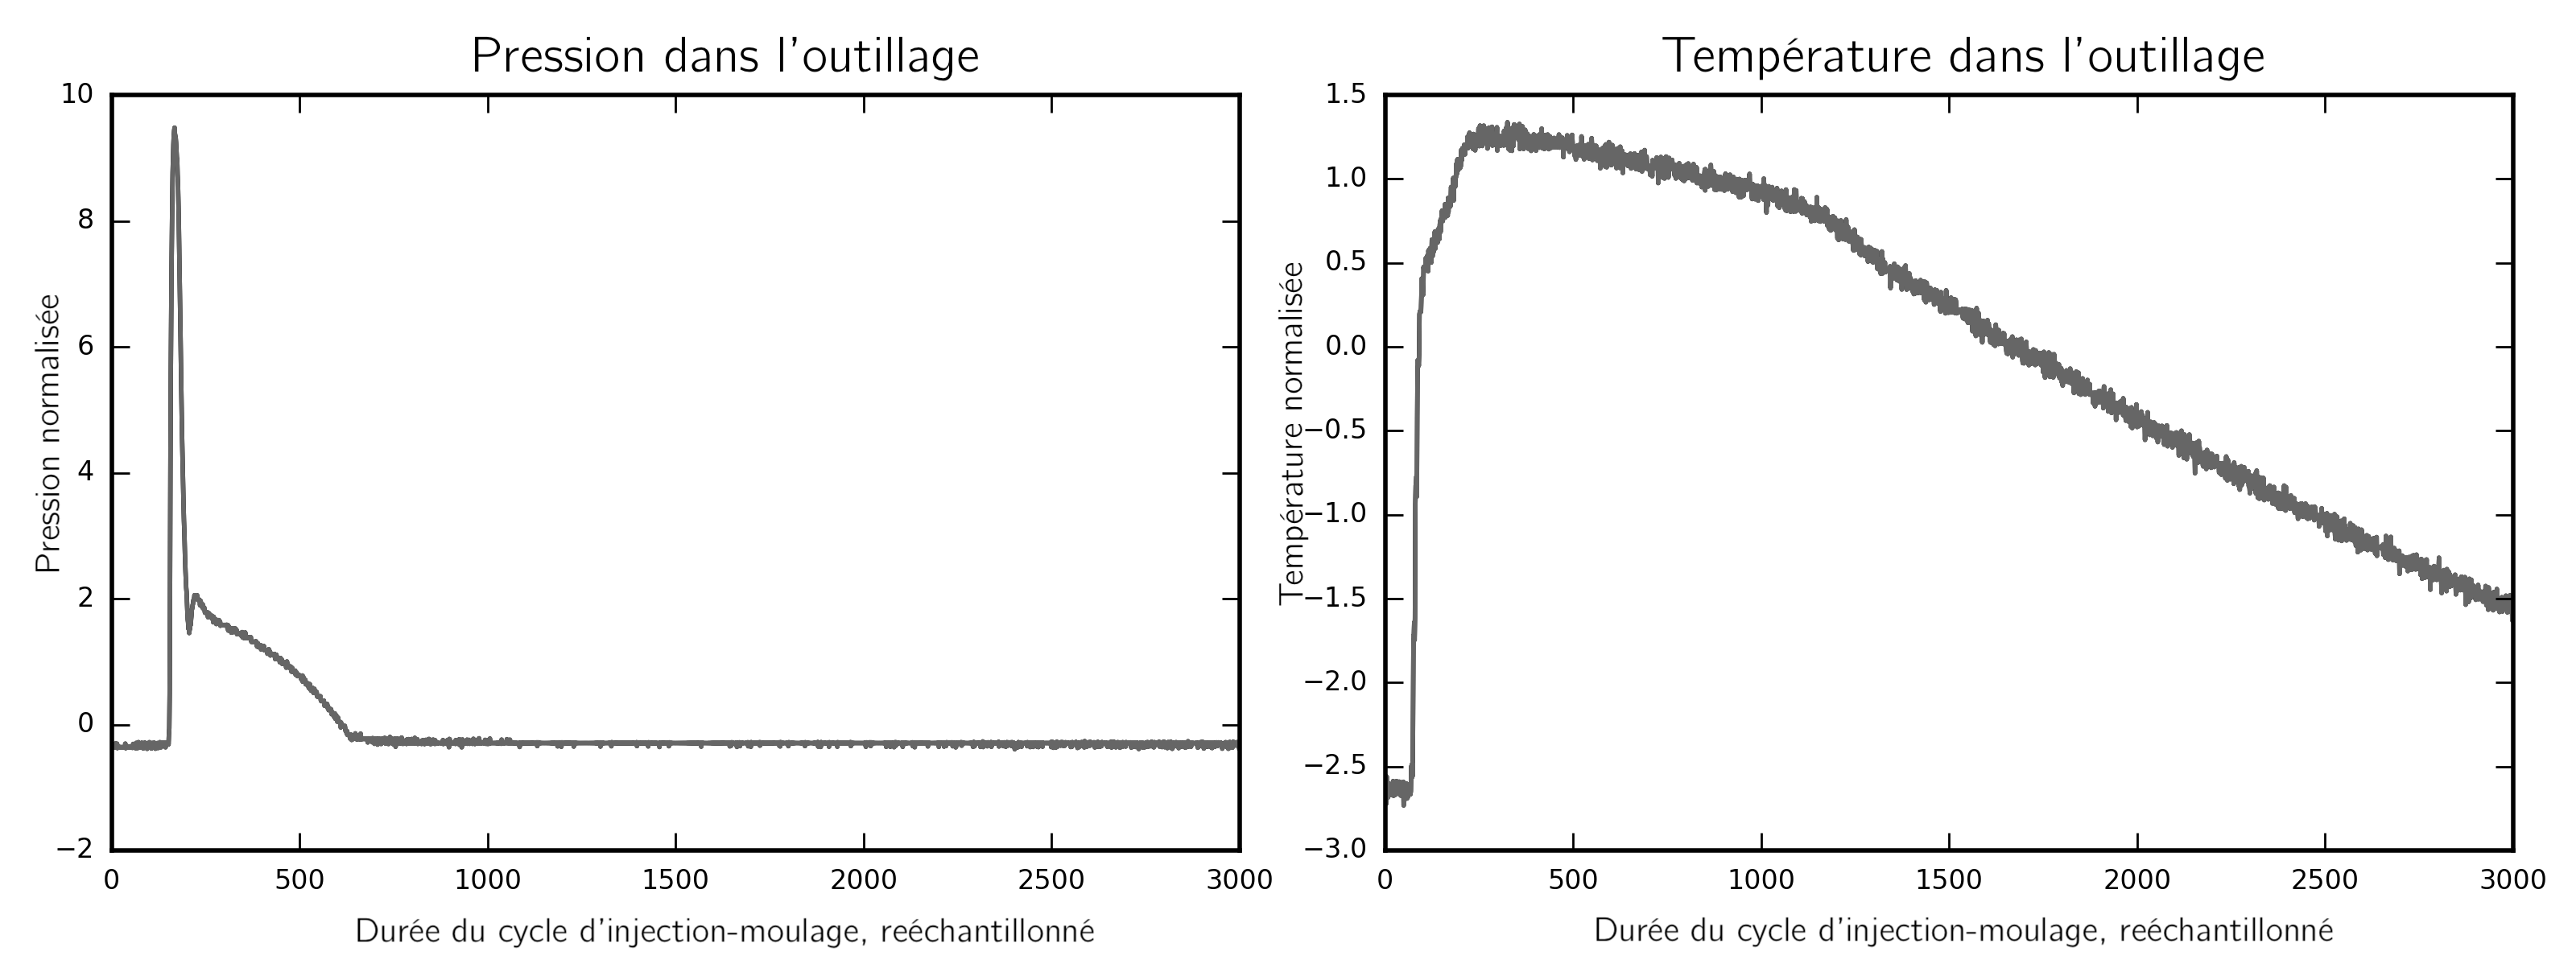
\includegraphics[width=\textwidth]{../Chap2/Figures/part1_std_signals.png}
	\caption{Résultats de mesure de la pression et la température dans l'outillage pendant tout le cycle.}
	\label{fig:inmold_signals}
\end{figure}

% TODO: remove this study?
Nous nous appuyons sur une production de 204 pièces, pendant laquelle les paramètres de la machine ont variés suivant un plan d'expériences de criblage, discuté dans le Chapitre \ref{ch:dataset} §\ref{subsec:l12_doe} à venir.
Le modèle qui prédit au mieux la géométrie à partir des mesures s'appuie sur des réseaux de neurones récurrents. % \textit{LSTM}.
La Figure \ref{fig:signals_lstm} présente les résultats normalisés obtenues par validation croisée\footnote{Nous détaillons le principe de la validation croisée dans l'Annexe \ref{subsubsec:cross_val}.}, pour 27 pièces de la base de données de validation.
L'erreur de prédiction est faible.
Cela correspond à une erreur moyenne de prédiction de la dimension de 1,3 millimètres sur une dimension de 90 millimètres, soit une erreur relative de 1,54\%.
Ces résultats montrent l'intérêt de ce type de mesure indirecte des caractéristiques du produit.
Cette erreur est inférieure aux tolérances générales des pièces plastiques donnée dans la norme ISO20457 \cite{ISO_20457_2018}, qui exige entre 2\% et 4\% d'écarts dimensionnel.
% Toutefois, si elle est généralisée pour des pièces dont les dimensions font un mètre, une erreur relative de 1,54\% est équivalente à une erreur de 1,54 centimètres.
% Aussi, l'erreur obtenue par le modèle est à la limite de faisabilité de l'employer comme moyen de contrôle prédictif de la géométrie.
% Il faudrait une erreur dix fois moindre pour garantir la possibilité d'utilisation de ce modèle prédictif.
% Un jeu de données de pièces plus conséquent, ainsi qu'un modèle plus raffiné, sont des pistes pour améliorer ces performances.

Dans une démarche de surveillance de l'état du procédé d'injection-moulage, la mesure de variables sur la machine est importante.
Une mise sous surveillance statistique MSP\footnote{Nous présentons la littérature sur la surveillance statistique MSP en injection-moulage dans l'Annexe \ref{subsubsec:spc}.} permet de détecter les situations hors-contrôle.
Nous invitons le lecteur qui s'intéresse aux mesures réalisées sur le procédé plutôt que sur le produit, à consulter l'état de l'art récent et exhaustif de \citeauthor{ageyeva_inmold_2019} \cite{ageyeva_inmold_2019}.
% Nous ajoutons la possibiliter d'analyser les vibrations de la machine.

\begin{figure}[bthp]
	\centering
	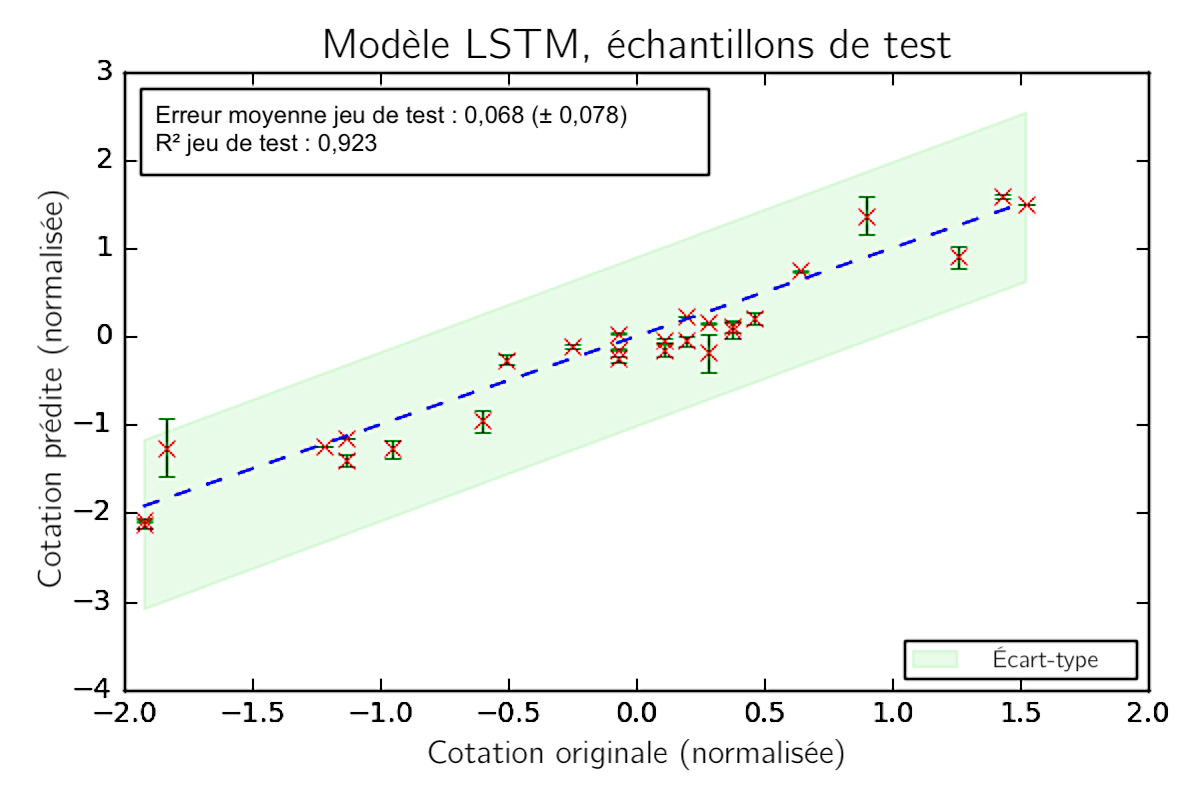
\includegraphics[width=0.8\textwidth]{../Chap2/Figures/1LSTM_Cross_val_MSE_013splited_Ystd.png}
	\caption{Résultats du modèle LSTM sur le jeu de données de test.}
	\label{fig:signals_lstm}
\end{figure}

%Dans notre objectif, nous cherchons à mesurer les caractéristiques d'aspects des pièces.
%À la différence de notre travail sur la prédiction d'une cotation géométrique, les caractéristiques d'aspect sont difficilement représentées par une unique variable continue.
%La représentation des caractéristiques d'aspect la plus commune est l'image numérique.
%Elle se compose de plusieurs milliers de valeurs entières discrètes, généralement encodées sur 8 bits (entre 0 et 254).
%Nous n'avons pas réussi à construire un modèle qui prédit les caractéristiques de l'aspect des pièces à partir des seules mesures dans le moule.
%Aussi, nous pensons qu'il est nécessaire de capturer une image de l'aspect des pièces, dès leur sortie du moule, afin d'établir une mesure de l'aspect.
%La mesure directe est l'objet de la section suivante.

Un capteur intégré dans le moule est associé un outillage, et donc à une unique pièce.
Il n'est pas viable de démonter le capteur pour le positionner sur un autre outillage.
À contrario, un dispositif de mesure extérieur au procédé n'est pas lié à un outillage.
% Cela permettrait de contrôler la qualité quand le cahier des charges le nécessite, quelle que soit la pièce produite.

\subsection{Mesurage direct des caractéristiques du produit}
% \subsection{Faisabilité technologique du mesurage de la qualité en ligne de production}
%Pour identifier un modèle du procédé, il est nécessaire de réaliser des mesurages afin de connaître l'état de celui-ci à différents instants.  % discrets.
%Afin de pouvoir analyser l'évolution du procédé, l'échantillonnage des mesures doit être supérieure au temps caractéristique d'évolution du procédé.
%Dans le cas de l'injection-moulage, l'évolution à court-terme du procédé est souvent proche d'une dizaine de cycles de production, soit de 100 à 600 secondes.  % soit le temps de cycle du procédé
%Dans le cadre de notre travail, nous choisissons de réaliser le contrôle de cent pourcent des pièces.
%Le mesurage doit être réalisé pendant la durée du cycle d'injection-moulage.
%% Aller capter des infos qui sont porteuses de l'info de non-conformité mais qui ne sont pas
%Pour respecter cette contrainte, nous distinguons deux grands types de mesures :
%\begin{itemize}
%\item les mesures dites "invasives", qui nécessite l'installation de capteurs de grandeurs physiques à l'intérieur de l'outillage et de la presse,
%\item les mesures "non-invasives", qui s'intéressent à la pièce produite dès qu'elle sort de l'outillage et à l'extérieur de la presse.
%\end{itemize}
%
%% Les capteurs dans le moule peuvent mesurer la pression, la température ou bien la vitesse de déplacement de la matière par effet Doppler.
%% En 2019, les systèmes d'acquisition utilisés avec ces capteurs fonctionnent à une fréquence de 25 à 1000 Hertz.
%% Ainsi, le nombre de valeurs discrètes mesurées pendant un cycle est de l'ordre de dix milles.
%
%Les mesures "invasives" nécessitent un travail de conception de l'outillage compliqué.
%L'outillage intègre des canaux de refroidissement et le câblage des capteurs doit être conçu pour les éviter.
%C'est pourquoi, \citeauthor{gao_multivariate_2012} proposent un capteur qui communiquent sans connectivité filaire \cite{kazmer_feasibility_2011, gao_multivariate_2012}.
%L'outillage en acier conducteur est une cage de Faraday idéale.
%La communication radiofréquence  est impossible.
%C'est pourquoi leur capteur utilise des ondes acoustiques pour communiquer.
%L'alimentation en énergie est assurée en récupérant les variations de pressions créées lors du cycle l'injection.
%Cependant, cette solution n'est pour l'instant pas commercialisée.
%
%De plus, la maintenance des capteurs intégrés à l'outillage est compliquée.
%Les capteurs sont fragiles et les contraintes physiques qui s'exercent sur eux lors du cycle d'injection sont élevées.
%En particulier, nous avons observé pendant nos campagnes d'essais que les défaillances proviennent le plus souvent des câbles et non des capteurs eux-mêmes.
%En cas de défaillance d'un capteur, c'est l'ensemble de l'outillage qui est immobilisé, ce qui impacte fortement la production industrielle.
%À contrario, le mesurage des pièces, dès leur sortie de l'outillage, ne demande pas ce travail de conception avancée.
%Le système de mesure non-invasif est éloigné des contraintes physiques du procédé d'injection-moulage, ce qui limite le besoin de maintenance.
%% Un système de mesure avec des imageurs est positionné en sortie de moule afin de mesurer la pièce.
%% L'objet de ces travaux de thèse est le développement d'un système de mesure non invasif de la qualité des pièces produites.
%% Cette démarche s'inscrit dans une réduction des coûts de l'instrumentation des moules et dans une logique de mesure directe de la qualité géométrique et d'aspect visuel de la pièce au plus tôt dans la chaîne de production.

Le mesurage de la pièce permet d'obtenir directement une information sur ses caractéristiques ; à la différence du mesurage de variables dans le moule, qui ne sont que des indicateurs de la qualité.
% Nous détaillerons l'intérêt du contrôle non-invasif de la qualité dans le Chapitre \ref{ch:measure}.

Pour être intégrée à la ligne de production et contrôler cent pourcent des pièces, le mesurage des caractéristiques du produit doit être réalisé dans une durée inférieure au temps de cycle du procédé d'injection-moulage pour que cela soit viable économiquement.
% Cette contrainte permet de réaliser le contrôle de cent pour-cent des pièces.
Si la pièce doit être déplacée devant le moyen de mesure, la durée du convoyage doit également être incluse dans cette durée.
De plus, si on souhaite écarter la pièce non-conforme de la chaîne de production, il est alors nécessaire d'effectuer l'analyse de résultat pendant la durée du cycle.
% Ces contraintes réduisent d'autant plus la durée disponible pour réaliser la mesure.
% Nous estimons que la durée maximale de la mesure est de 10 secondes pour une durée du cycle de production de 60 secondes.
La Figure \ref{fig:time_constraint} inscrit la durée de mesurage dans le chronogramme du cycle du procédé.  % (Figure \ref{fig:chronogramme}).
Cette contrainte de durée de mesurage sera une contrainte forte pour l'ensemble des choix technologiques de nos travaux.

\begin{figure}[tbhp]
	\centering
	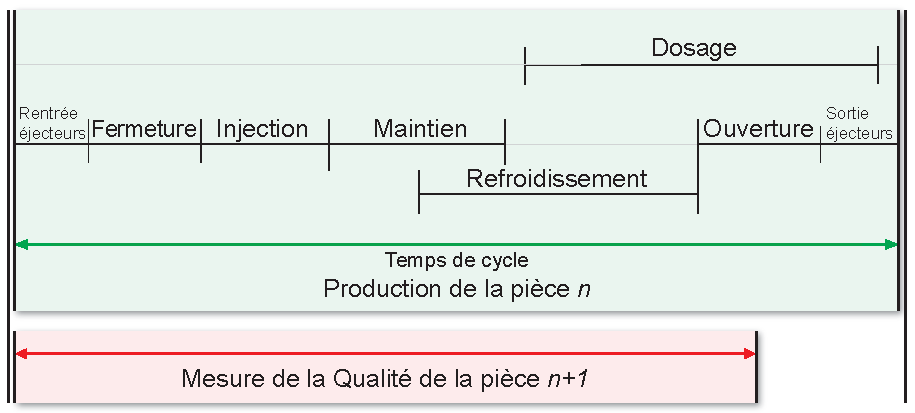
\includegraphics[width=0.82\textwidth,height=\textheight,keepaspectratio]{../Chap1/Figures/SAPRISTI_Chronogramme-Simple.pdf}
	\caption{Intégration de la mesure dans le cycle d'injection-moulage.}
	\label{fig:time_constraint}
\end{figure}

Différentes mesures sont aujourd'hui compatibles, de par leurs courtes durées, avec une utilisation en cycle industriel : pesée de la masse ; imagerie par thermographie infrarouge ; contrôle d'aspect par caméras ; imagerie tridimensionnelle \cite{schwenke_optical_2002} ; durométrie ; imagerie des champs de contraintes par les phénomènes de photoélasticité sur les pièces plastiques transparentes.
% Pour obtenir des résultats fiables la mesure doit être automatisée.
% C'est un des objectifs de nos travaux.

% La réalisation d'un système de mesure des caractéristiques des pièces dès la sortie du moule est un des objectifs de nos travaux.
% Nous discuterons de manière approfondie des techniques de mesure existantes dans le Chapitre \ref{ch:measure}.


%Quelles sont les propriétés physico chimique que l'ont peut regarder ?
%Mécanique (masse, Vibratoire, dimensions, sonores),  electromag. (thermique: pour tout ce qui est pièces chaudes, visuel, polarisé).
%Attention : mesurande différent mesurée
%4 - Limites de la mesure avec contact physique
%
%4 - Mesures sans contact
%- XRay tomography
%- Ultrasound
%- Confocal microscopy
%- Thermography, active or passive
%- Polarimetry
%- Laser triangulation (3D scanning)
%- TheraHertz imaging
%
%\section{Imagerie hyper-spectrale}
%\subsection{Spectre Rayon X}
%\blindtext
%
%\subsection{Spectre Visible}
%\blindtext
%
%\subsection{Spectre Infrarouge : Thermographie}
%\blindtext
%
%\subsection{Spectre Térahertz}
%\blindtext
%
%\section{Imagerie non-conventionnelle}
%\subsection{Light-Field}
%\blindtext
%
%\subsection{Polarimétrie}
%\blindtext
L'approche de nos travaux consiste à mesurer les caractéristiques des pièces dès la sortie de la presse d'injection-moulage.
La réalisation de ces mesures nécessite de convoyer la pièce devant le banc de mesure.
Un tapis roulant ou un bras robotisé permet de déplacer la pièce.
% La durée des déplacement est à prendre en compte, vis à vis de la durée du cycle et de la durée de la mesure.
% De nombreuses méthodes ont été développées pour mesurer les propriétés mécaniques des pièces.

Dans nos travaux, nous n'utiliserons pas de méthodes de mesure invasives, ni de mesures réalisées hors-ligne.
L'étude de ces méthodes peut néanmoins servir d'inspiration pour concevoir des méthodes de mesure non invasives et sans destruction des pièces.
Ainsi, nous nous intéresserons dans nos travaux à la polarimétrie et à la thermographie.
En revanche, nous n'étudierons pas l'utilisations des rayonnements X et Térahertz, car les machines restent coûteuses.
Nous discutons dans cette section de l'utilisation de différents moyens de mesure en ligne de production.
Les apports de la thermographie et de la polarimétrie seront détaillés dans le Chapitre suivant Section \ref{subsec:thermography} et Section \ref{subsec:polarimetry}.

Nous proposons une liste des principales caractéristiques qui peuvent être mesuré sur une pièce plastique :
\begin{itemize}
	\item contraintes internes,
	\item contraintes internes,
	\item structure cristalline de la matière,
	\item densité,
	\item état de surface,
	\item géométrie.
\end{itemize}

\subsubsection{Mesurage des contraintes internes}
La mesure des contraintes résiduelles dans la pièce est un enjeu important car elles fragilisent les pièces.
La thèse de doctorat de \citeauthor{giroud_mesure_2001}, intitulée \citetitle{giroud_mesure_2001}, propose de mesurer les contraintes internes d'une pièce à l'aide de la méthode de l'enlèvement de couches fines \cite{giroud_mesure_2001}.
C'est une méthode qui détruit la pièce et qui doit être réalisée en dehors de la ligne de production.

\subsubsection{Mesurage cristallographique}
La mesure des caractéristiques cristallographiques est importante car ce sont ces caractéristiques qui déterminent les propriétés mécaniques des pièces.
% Cette structure est dépendante des paramètres du procédé.
\citeauthor{mendoza_spatial_2003} utilise par exemple la polarimétrie sur couche mince (micrographie) pour mettre en évidence les axes d'orientation du polymère semi-cristallin \cite{mendoza_spatial_2003}.
Dans ces travaux de thèses, \citeauthor{malhab_moulage_2012} introduit l'utilisation de la diffraction des rayons X à grands et petits angles, à l'aide d'un rayonnement synchrotron hautement énergétique (12 KeV) \cite{malhab_moulage_2012}.
% Wang et Cakmak (2001) ont utilisé des échantillons qui avaient une géométrie parallélépipédique.
% L’étude approfondie de la morphologie cristalline a été réalisée à partir de mesures de diffusion des rayons X aux petits angles (SAXS) et de diffraction des rayons X aux grands angles (WAXS). Une analyse dans l’épaisseur des micro-plaques à nécessité l’utilisation d’un faisceau X de faible épaisseur (30μm) que seul un synchrotron peut facilement délivrer.
La cohérence du faisceau synchrotron (30 micromètres) permet de mettre en évidence la structure cristallographique dans l'épaisseur des échantillons plastiques.
Cela permet d'étudier l'évolution de la structure en fonction des paramètres du procédé d'injection.
La diffraction à grands angles (\textit{Wide-Angle X-ray Scattering}) permet de déterminer le degré de cristallinité du polymère semi-cristallin, en observant les figures de diffraction de la structure cristalline.  % subnano, aux dimensions picométriques, Bragg peaks
La diffraction à petits angles permet de déterminer les dimensions nanomètriques de la structure du polymère, telles que la longueur de la période de répétition du motif cristallin, la largeur et la longueur de la lamelle cristalline.
À partir de la structure cristalline, il est possible de diagnostiquer des défauts structurelles et d'expliquer leurs causes en terme de variables du procédé de production (viscosité de la matière, pression d'injection, températures ...).

\subsubsection{Mesurage de la densité}
En 2010, le projet \textit{PLASTX} du Pôle Européen de la Plasturgie\footnote{Le Pôle Européen de la Plasturgie est devenu le \href{https://ct-ipc.com/}{Centre Technique Industriel de la Plasturgie et des Composites} (IPC) en 2017.} propose de réaliser une mesure par tomographie rayons X des pièces dès leur sortie du moule\footnote{\href{https://vimeo.com/50358748}{Vidéo de présentation} du démonstrateur du projet PLASTX.}.
La source de rayons X est fixe et un bras robotique déplace la pièce dans un mouvement de rotation.
La tomographie permet de mesurer le champ de densité de la pièce.  % par la transformée de Radon.
Les résultats du projet \textit{PLASTX} montrent que cette mesure est compatible avec le temps de cycle industriel.
Cependant, la mise en place d'une source de rayons X sur une ligne de production reste difficile en raison des blindages nécessaires.

\subsubsection{Mesurage de l'état de surface et de l'aspect}
En 2009, le projet européen \textit{poliMATIC}\footnote{Projet de recherche de la Commission européenne FP7-NMP-2009-SME-3 : \href{https://www.automated-polishing.eu/}{automated-polishing.eu}} a proposé de robotiser l'utilisation de la microscopie confocal (\href{https://www.altimet.fr/?page_id=248}{capteur Altimet} de la société Altisurf) pour contrôler la rugosité de pièces.
La position du capteur est asservie en distance pour mesurer des pièces courbes.
Un interféromètre portatif\footnote{Interféromètre désormais commercialisé par la société \href{http://qisab.com/}{QiSab}} a également été développé pour améliorer la résolution et atteindre une précision inférieure au nanomètre \cite{baath_new_2012}.
La durée de la mesure est élevée, car le capteur mesure une surface de $4\times 4$ centimètres.
Il doit être déplacé sur toute la surface.

% WAXS (détermination du taux de cristallinité) et SAXS (identification de la longue période, de l'épaisseur des lamelles cristallines et de la phase amorphe interlamellaire)
Dernièrement, dans ses travaux de doctorat, \citeauthor{lacombe_exploitation_2018a} utilise un dôme de mesure de la réflectance (\textit{Reflectance Transformation Imaging}) pour contrôler les caractéristiques d'aspect de pièces plastiques \cite{lacombe_exploitation_2018a}.
Ce dôme de réflectance n'est actuellement pas intégré à la ligne de production, à cause de ses dimensions.
Des travaux sont actuellement en cours pour proposer une méthode d'intégration en ligne de production.

\subsubsection{Mesurage géométrique par triangulation laser} \label{subsec:scan3D}
% Il demande un équipement calibré et automatisé.
% Il prend place après la production et il permet d'exclure les pièces non conformes.
% Ce contrôle dimensionnel ne s'intéresse pas à l'aspect des pièces, uniquement aux profils géométriques.
% En pratique, le contrôle dimensionnel est généralement réalisé par un humain à l'aide d'un comparateur.
% Le coût et la complexité de l'installation de l'imagerie de profil réserve cette méthode automatique aux productions à haute valeur ajoutée.
Le contrôle dimensionnel de profil plan peut être automatisé par imagerie de profil.
Dans le cas de pièces moulées, les caractéristiques géométriques sont souvent tridimensionnelles.
Il est alors nécessaire de réaliser le mesurage de plusieurs profils orthogonaux, où bien d'utiliser un moyen de mesure tridimensionnel.

\begin{figure}[htbp]
	\centering
	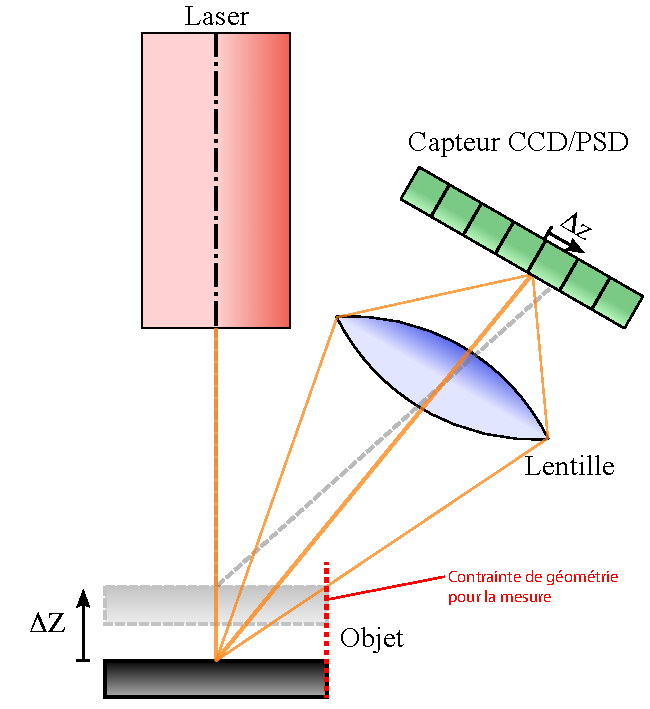
\includegraphics[width=0.45\textwidth]{../Chap2/Figures/Laserprofilometer_FR.pdf}
	\caption[Mesure de la géométrie d'un objet par triangulation laser.]{Mesure de la géométrie d'un objet par triangulation laser. Figure dérivée du \href{https://commons.wikimedia.org/wiki/File:Laserprofilometer_EN.svg}{travail original} de \href{https://de.wikipedia.org/wiki/Benutzer:Xorx}{Georg Wiora (Dr. Schorsch)}, \href{http://creativecommons.org/licenses/by-sa/3.0/}{CC BY-SA 3.0, via Wikimedia Commons}.}
	\label{fig:laser_scanning}
\end{figure}

Il existe un grand nombre de moyens de mesure pouvant être qualifiés de scanner tridimensionnel.
Nous distinguons les méthodes avec contact physique de la pièce et sans contact, qui utilisent la réflexion ou la transmission d'une onde électromagnétique.  % (Machines de Mesure Tridimensionnelle)
Dans le cadre de la mesure sans contact, les moyens les plus employés sont la stéréoscopie, la photogrammétrie, la lumière structurée, la tomographie, le temps de vol et la triangulation laser.

La triangulation laser s'appuie sur la mesure d'un écart de parallaxe entre d'une part, une source laser balayée linéairement par un galvanomètre, et d'autre part la réflexion du laser sur l'objet à mesurer.  % communément appelée "scanner 3D"
Une source lumineuse laser est choisie car la largeur du faisceau lumineux sur la pièce doit être la plus petite possible.
Le faisceau laser cohérent garantit une dispersion angulaire faible à grande distance.

La Figure \ref{fig:laser_scanning} présente le principe de la mesure par triangulation.
Un écart géométrique verticale $\Delta Z$ entraine un écart proportionnel, sur le plan du capteur.
La méthode de triangulation laser souffre de quatre contraintes principales :
\begin{itemize}
	\item L'intensité lumineuse du laser doit être supérieure à la luminosité ambiante. C'est pourquoi la longueur d'onde du laser est souvent choisie hors du spectre visible.
	\item La fréquence de balayage du laser doit être très supérieure au déplacement de la pièce. Cela conditionne la fréquence d'acquisition du capteur.
	\item Le matériau qui est mesuré doit avoir une absorption faible pour la longueur d'onde du laser et les réflexions spéculaires directes doivent être évitées.
	\item La géométrie de la pièce doit permettre la mesure : elle ne doit pas entrainer d'occlusion pour le couple source laser et capteur. L'écart angulaire de ce couple est souvent proche de 45°. C'est pourquoi les géométries concaves doivent être supérieures à 45°.
\end{itemize}

La Figure \ref{fig:online_scan} présente notre mise en place de cette mesure, en cycle industriel.
Le scanner tridimensionnel que nous utilisons est le \textit{Handyscan 3D ZSCANNER 700}\footnote{\href{https://www.creaform3d.com/fr/soutien-la-clientele/produits-retires/handyscan-3d-de-1re-generation-zscanner-700}{Caractéristiques techniques} du scanner Handyscan 3D ZSCANNER 700 sur le site du fabricant Créaform.}.
% How HandyScan works: https://www.creaform3d.com/sites/default/files/assets/technological-fundamentals/teaching_manual_reverse_engineering_en_18032014_6.pdf
% Nous avons évalué la répétabilité de ce scanner à 100 micromètres.
% Une pièce étalon a été mesurée sur une machine de mesure tridimensionnelle, puis elle est mesurée à l'aide du scanner.
% Les résultats ont été comparés à l'aide du logiciel GéoVérif \cite{pairel_maitrise_2016}.
La durée de la mesure est de 40 secondes.

\begin{figure}[bhtp]
	\centering
	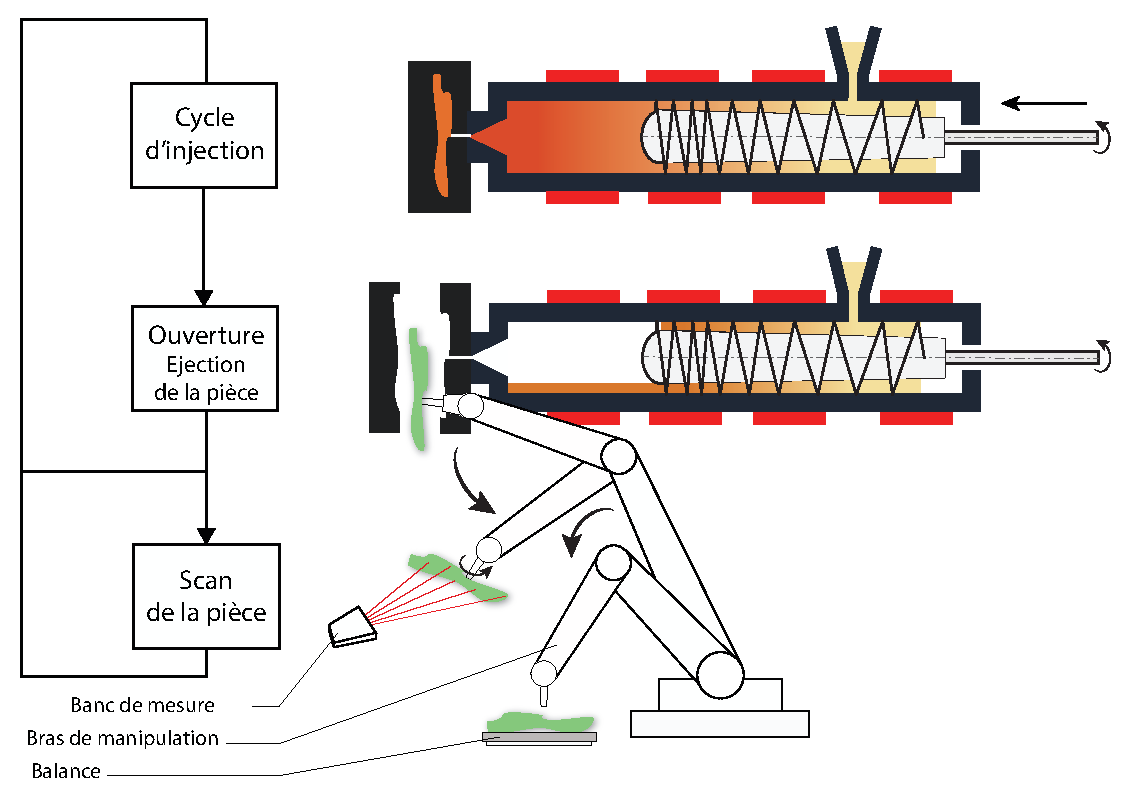
\includegraphics[width=0.8\textwidth]{../Chap2/Figures/online_scan.pdf}
	\caption{Mesure de la géométrie d'un objet par triangulation laser en cycle industriel.}
	\label{fig:online_scan}
\end{figure}

\begin{figure}[thbp]
	\centering
	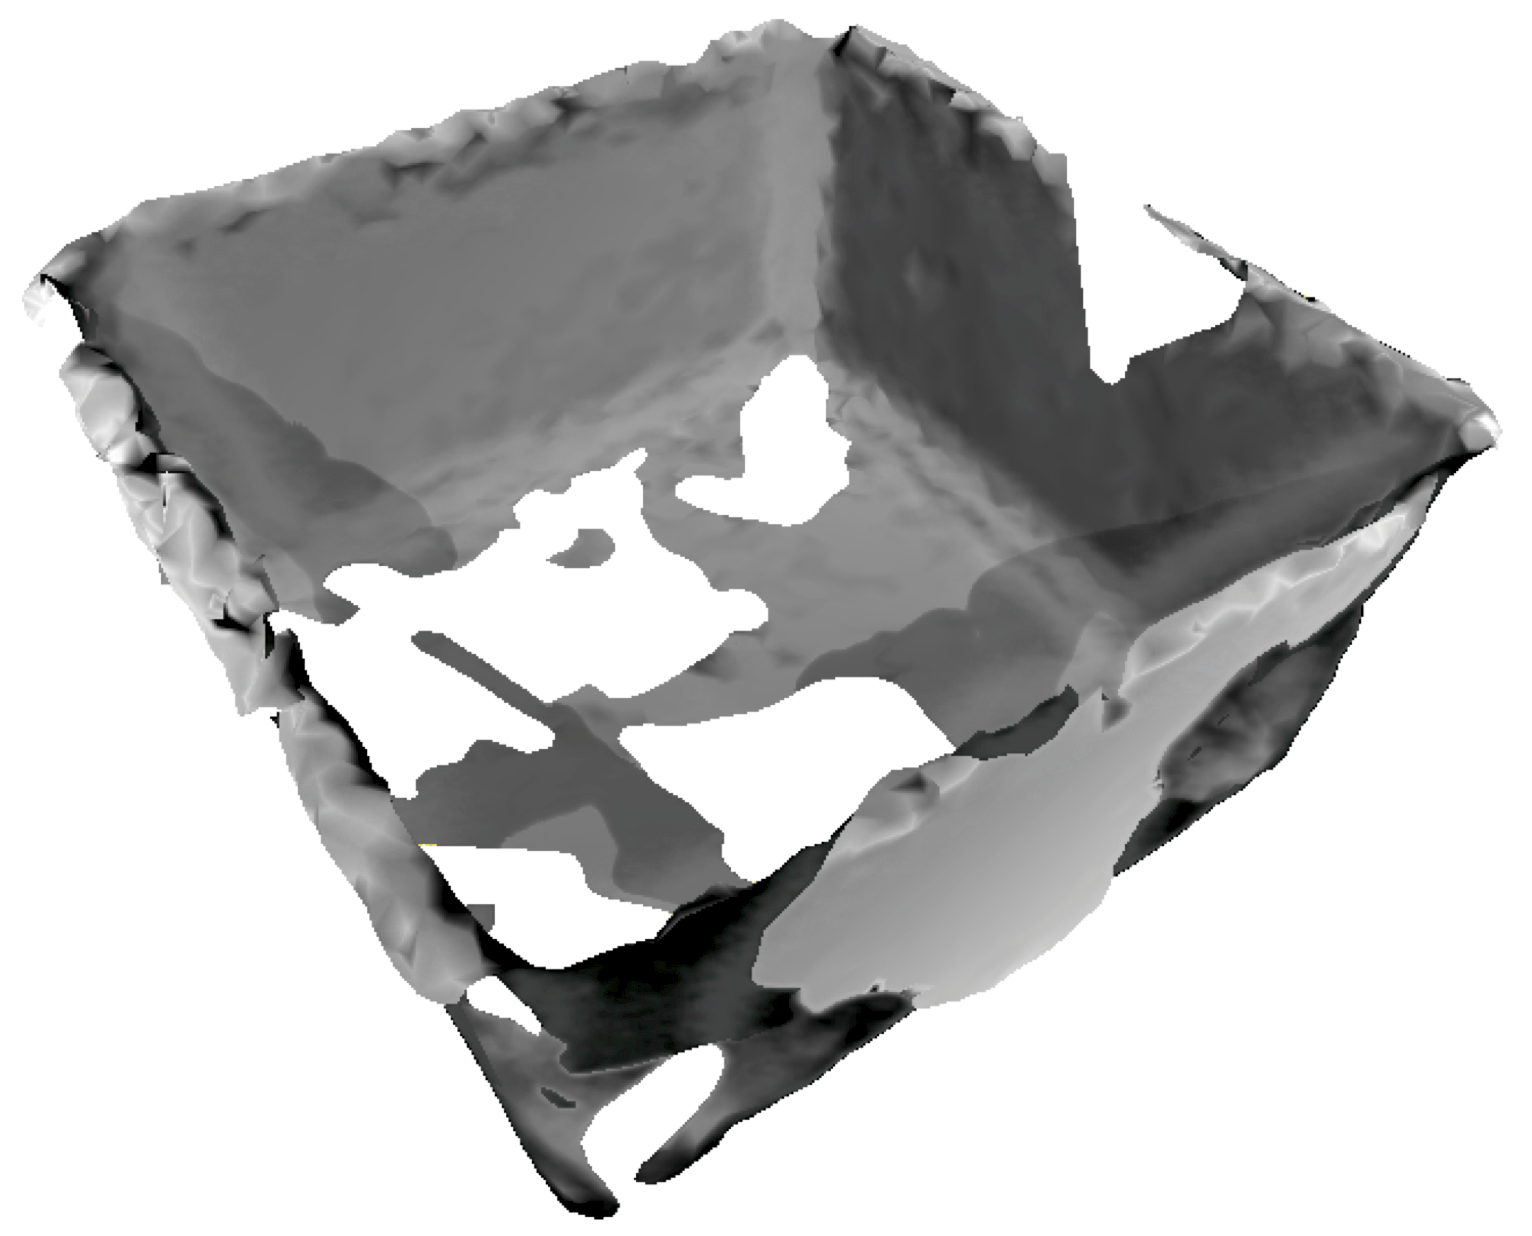
\includegraphics[width=0.5\textwidth]{../Chap2/Figures/online_3d_scan.png}
	\caption{Nuage de points de la pièce obtenue en cycle industriel avec le HandyScan.}
	\label{fig:online_scan_result}
\end{figure}

Le scanner est fixe et une rotation complète de la pièce est exécutée devant le scanner, à l'aide du bras robotisé qui décharge la presse (voir Figure \ref{fig:online_scan}).
La vitesse de cette rotation définie la durée de la mesure, qui est elle même limitée par la durée cycle de production de la machine.
Un temps de cycle court impose de réaliser des déplacements rapides devant le scanner.

Le scanning de la pièce dès sa production permet de comparer la géométrie produite à la géométrie de référence de l'outillage.
La Figure \ref{fig:scan_delta} a. présente l'écart de la pièce chaude à la géométrie cible, qui est définie par le modèle de la conception CAO.

Dans notre cas d'application, la pièce mesurée possède des côtés qui occultent la réflexion du laser.
% Il est nécessaire de réaliser des rotations sous différents angles pour scanner toutes les surfaces de la pièce, ce qui nécessiterait plus d'un tour complet.
De plus, la vitesse de rotation que nous avons dû utiliser est trop élevée en comparaison de la fréquence de balayage du laser.
La Figure \ref{fig:online_scan_result} b. présente de scanning.
On observe la présence de trous dans le maillage des surfaces.
D'une pièce à l'autre, les trous n'apparaissent pas aux mêmes endroits sur la pièce.
Aussi, l'exploitation automatique d'une telle mesure est compliquée.
Un traitement manuel des nuages de points est requis.
Dans la suite de nos travaux, nous avons choisi de ne pas exploiter cette mesure à cause des performances non-adaptées de notre matériel.
L'étude de cette démarche de mesure devra être évaluée à l'aide d'un profilomètre laser ou d'un scanner tridimensionnel qui possède une fréquence de balayage laser plus rapide, afin de limiter les trous dans le nuage de points.

\begin{figure}[bhtp]
	\centering
	\begin{subfigure}[c]{0.49\textwidth}
		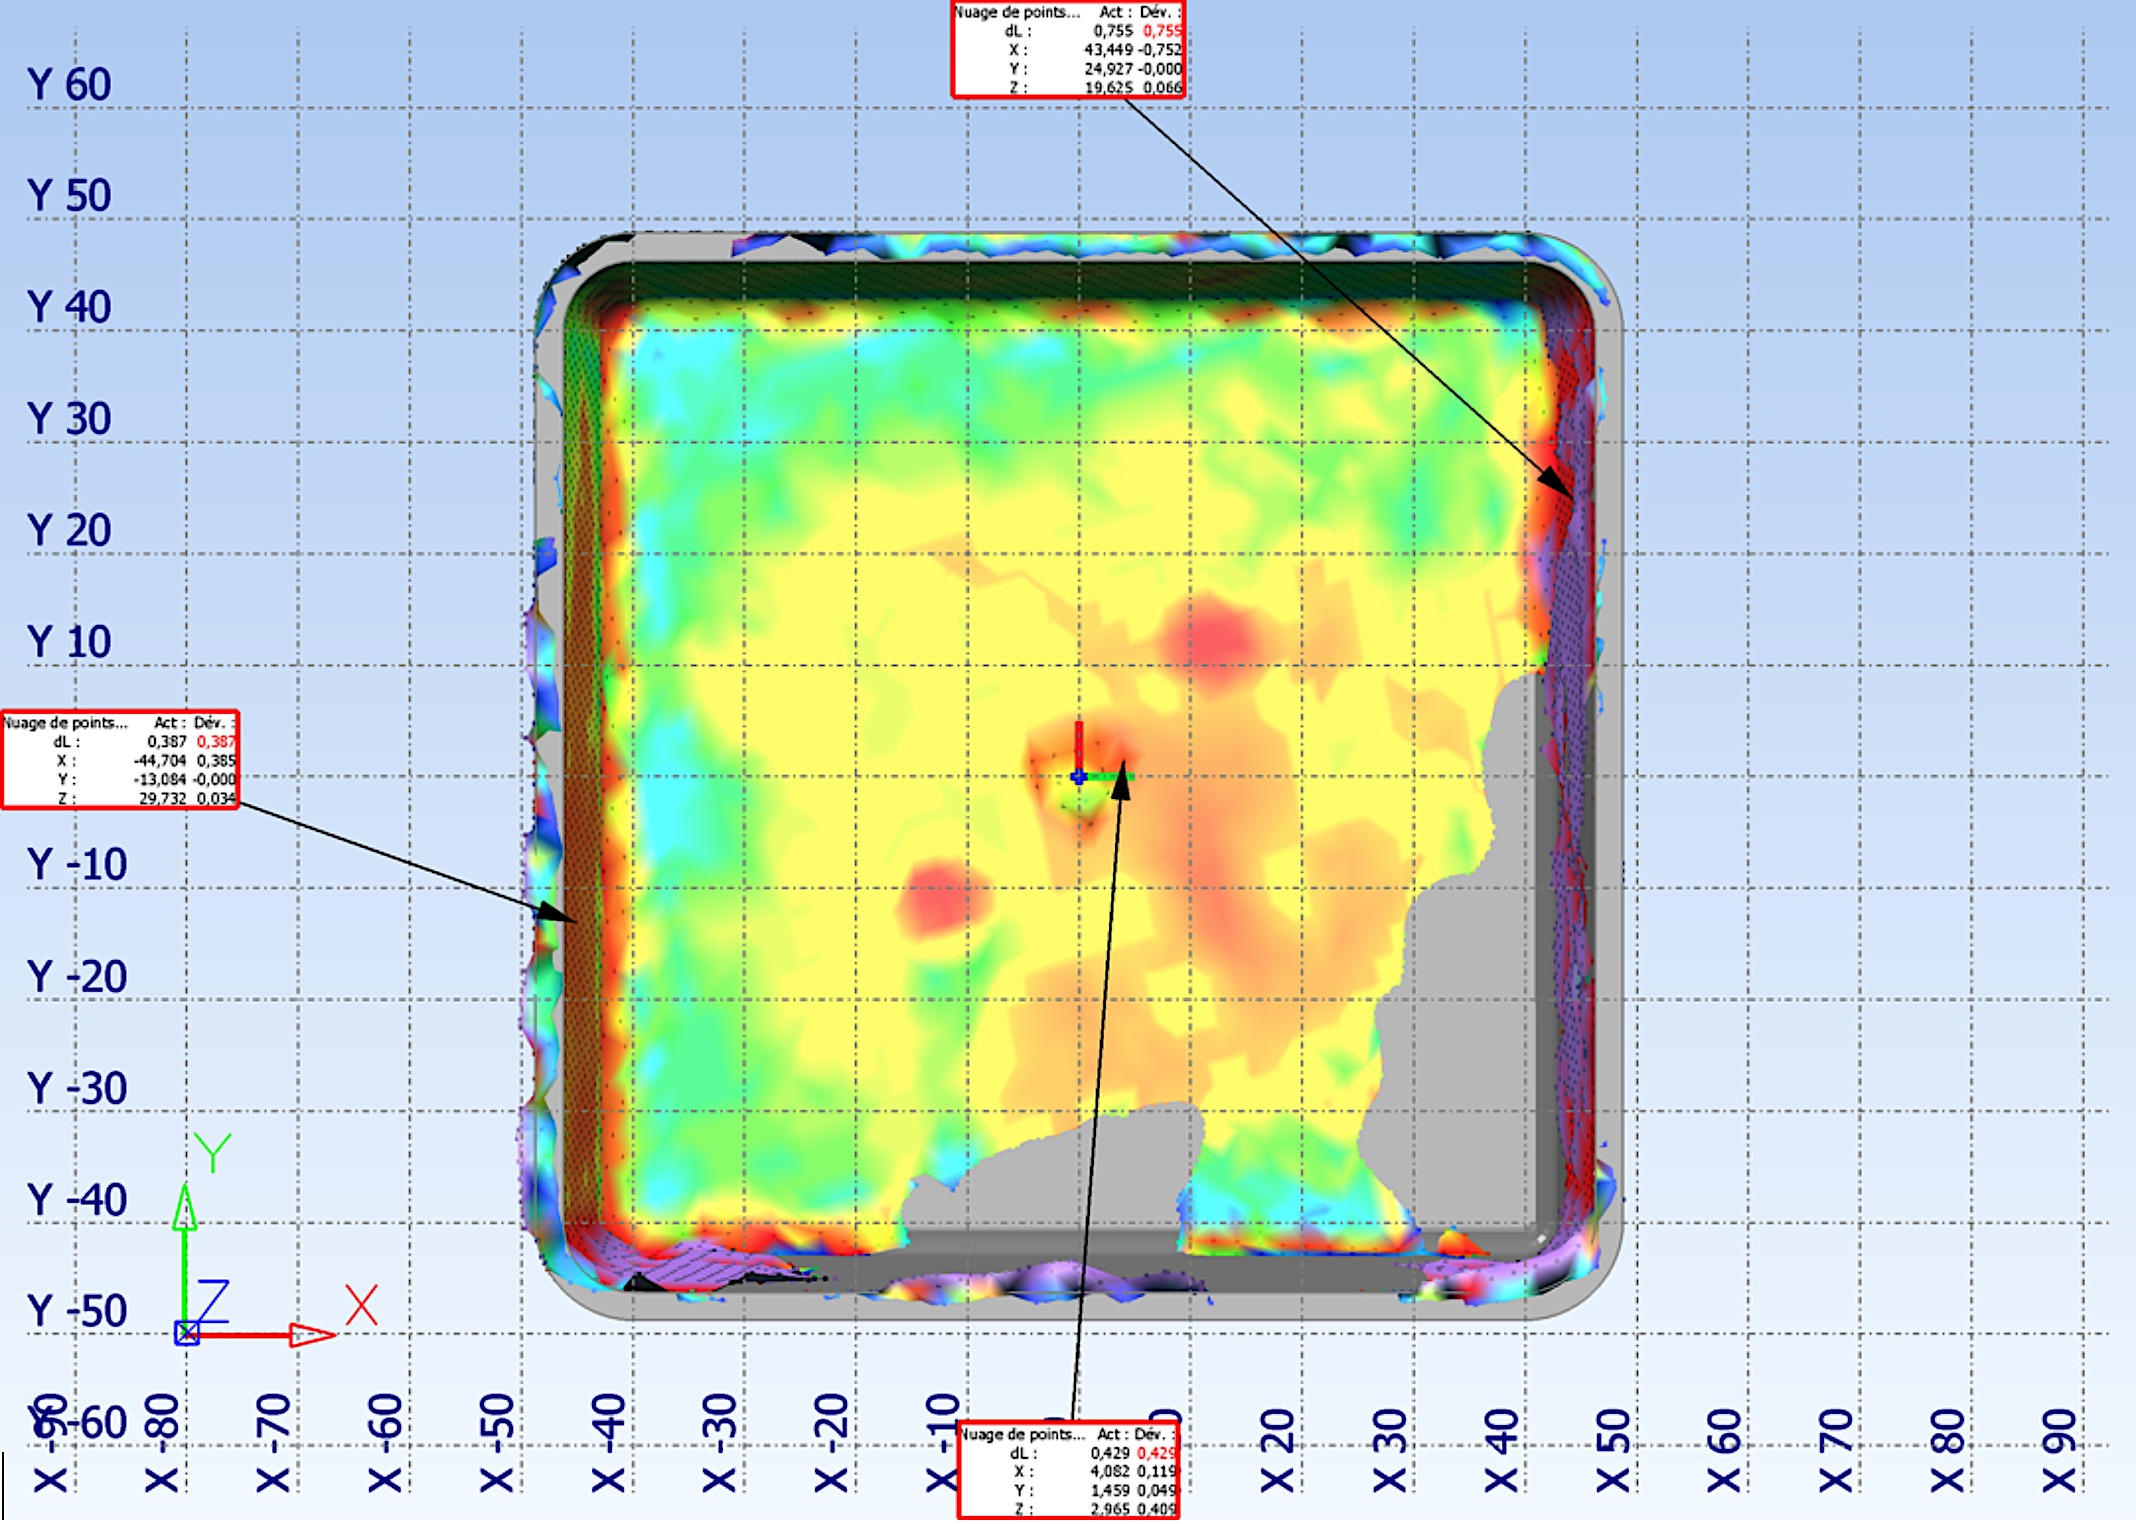
\includegraphics[width=\textwidth]{../Chap2/Figures/Capture_2019-09-23-13_43_11.jpg}
		\caption{Interpolation du nuage de points à l'aide du logiciel \textit{\href{https://www.autodesk.fr/products/powerinspect/}{PowerInspect2017}} de Autodesk.}
	\end{subfigure}
	\begin{subfigure}[c]{0.49\textwidth}
		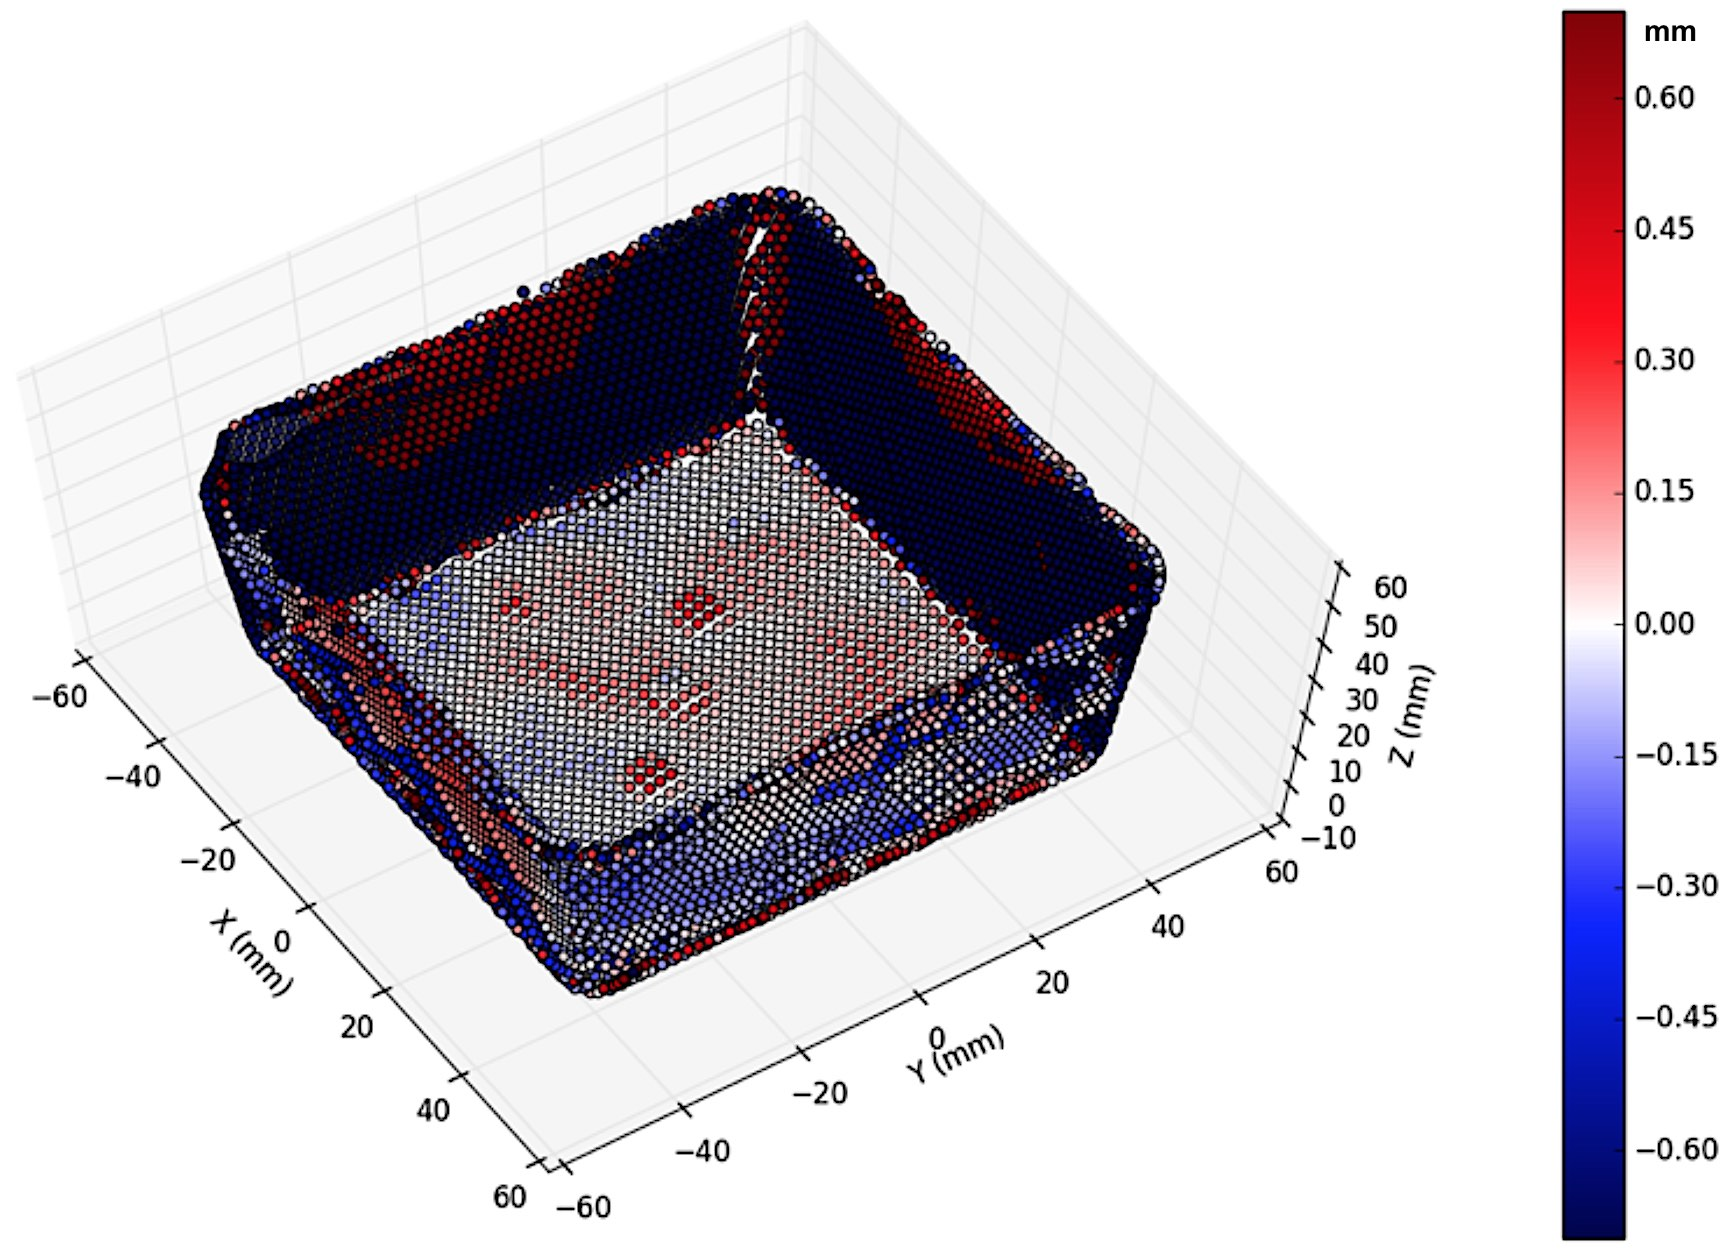
\includegraphics[width=\textwidth]{../Chap2/Figures/Capture_2019-09-23_13_42_00.jpg}
		\caption{Interprétation de l'écart des points de mesures à l'aide de la librairie Python \href{https://matplotlib.org/}{Matplotlib} \cite{hunter_matplotlib_2007, caswell_matplotlib_2019}.}
	\end{subfigure}
	\caption{Écart géométrique entre la pièce mesurée et la géométrie de référence de l'outillage.}
	\label{fig:scan_delta}
\end{figure}

Nous avons balancé le nuage de point à l'aide d'un critère de distance minimale entre les points et le modèle de référence (critère de moindres carrés).
Il est ainsi possible de caractériser les variations de la géométrie.
% Ce travail de doctorat n'a pas cherché à étudier le retrait.
% Nous supposons que le retrait est constant pour toutes les pièces d'un même lot.
% C'est néanmoins une information importante à exploiter pour la conception des outillages.
% Enfin, cette information est également très intéressante pour ajuster les paramètres du procédé afin d'obtenir une géométrie cible.

% En comparaison de l'imagerie thermique et polarimétrique, le coût du scanner tridimensionnel et la difficulté d'intégration de la mesure en ligne de production, sont bien plus importants.
% De plus, la répétabilité du scanner de 100 micromètres, rend difficile l'utilisation des mesures obtenues.
% Les déformations géométriques que nous observons sont de l'ordre de 100 micromètres.
% Les phénomènes de trous aléatoires dans le nuage de points compliquent l'interprétation automatique des mesures.
% Un traitement manuel des nuages de points est souvent requis.
% Or nous souhaitons automatiser la mesure de la qualité des produits.
% Pour toutes ces raisons, dans la suite de ce travail, nous avons choisi de ne pas poursuivre l'exploitation du scanner tridimensionnel HandyScan que nous avions à disposition.
% L'utilisation d'un tel moyen de mesure reste une piste de recherche très intéressante.

\subsection{Cahier des charges pour le contrôle de la qualité en ligne de production}
Dans le cas de pièces techniques, les exigences du client peuvent atteindre 3,4 pièces défectueuses par million de pièces (\textit{3,4 ppm} est la valeur couramment admise pour une approche « Six Sigma »).
Il est alors indispensable de réaliser le contrôle qualité sur cent pourcent des pièces, avant l'envoi au client.
Ce contrôle présente un coût et il devient intéressant de l'automatiser.

\begin{figure}[htbp]
	\centering
	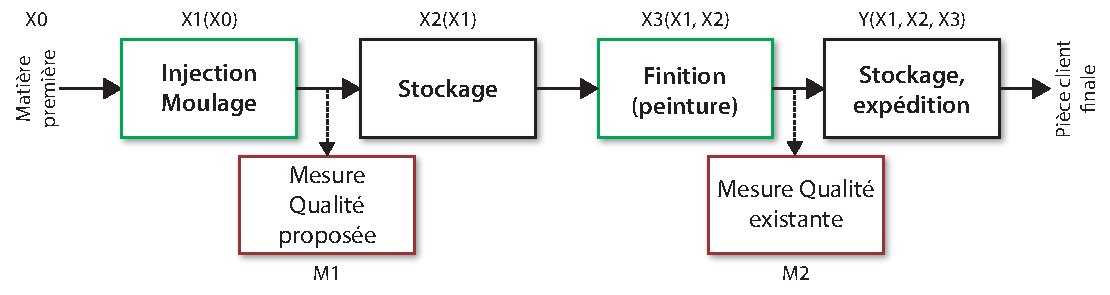
\includegraphics[width=\textwidth]{../Chap2/Figures/integration_controle_qualite.pdf}
	\caption{Intégration du contrôle de la qualité}
	\label{fig:quality_integration}
\end{figure}

La Figure \ref{fig:quality_integration} présente l'intégration du contrôle de la qualité au sein de la ligne de production.
Le contrôle de la qualité des produits est, de manière classique, réalisée après la finition des pièces.
L'état de la pièce dépend alors des étapes précédentes de finition $X3$, de stockage $X2$, de transport et de l'injection-moulage $X1$.
Des défauts peuvent apparaitre lors des phases de transports, stockages et de finitions.
Plus on multiplie le nombre d'étapes successives, plus il est difficile de trouver l'étape qui est la cause du défaut.
De plus, si la pièce est défectueuse à l'étape de l'injection-moulage $X1$, elle entraine des coûts de non-qualité : le coût du stockage de la pièce $X2$ et le coût de sa finition $X3$.
Le contrôle qualité en fin de chaîne de production ne permet pas d'éviter ces coûts.
Pour l'ensemble de ces raisons, nous proposons de réaliser la mesure de la qualité du produit dès la sortie du moule d'injection, alors que les pièces sont encore chaudes.
En plus d'éliminer les rebuts de la chaîne de production, il serait alors possible de construire un modèle de causalité entre les paramètres du procédé d'injection-moulage et les caractéristiques qualité de la pièce.
% Ce modèle permettrait d'ajuster les paramètres du procédé, pièces après pièces, pour optimiser la qualité.
% La construction de ce modèle et le pilotage du procédé d'injection-moulage ne sont pas l'objet de notre travail.
% C'est une perspective de recherche qui pourra s'inscrire à sa suite.

% \subsection{Vers une métrique de la qualité}
Le contrôle qualité est souvent réalisé de manière binaire : pièces conformes ou pièces non-conformes.
Occasionnellement, des grilles de notation à critères peuvent être utilisées pour attribuer une note de la qualité.
On réalise alors la moyenne géométrique de la note pour chacun des critères.
Ce processus de notation est néanmoins beaucoup plus long.
Il est réservé aux productions de pièces dont le prix de revient est élevé.
% Ainsi, la mesure de la qualité est rarement réalisée et on parle de contrôle (binaire) de la qualité.
% Les causes sont discutées dans le Chapitre \ref{ch:objectives} §\ref{sec:research_objectives}.
% Afin de réaliser une mesure de la qualité, notre travail propose également de définir une métrique de la qualité par apprentissage, à partir des données issues des capteurs, Chapitre \ref{sec:metric_learning}.

%Dans ce chapitre, nous discuterons du choix des capteurs à mettre en œuvre, pour mesurer en ligne de production.
%La littérature a proposé de réaliser des mesures indirectes\footnote{On parle d'une mesure indirecte lorsqu'il ne s'agit pas de mesurer directement la caractéristique de la pièce.
%La mesure de pression dans l'outillage est une mesure indirecte des caractéristiques finales de la pièces.
%C'est un indicateur des caractéristiques du produit.} de la qualité, comme par exemples des mesures de température ou de pression sur le moyen de production.
%% C'est pourquoi nous discuterons également de la pertinence des mesures.

%\begin{figure}[hbtp]
%	\centering
%	\begin{tikzpicture}
%	\begin{scope}[blend group=lighten] % blend group= soft light
%	% \fill[red!30!white]   ( 90:1.2) circle (2);
%	\fill[yellow!15!white]  (330:1.3) circle (2.4);
%	\fill[blue!15!white] (210:1.3) circle (2.4);
%	\end{scope}
%	% \node at ( 90:2)    {Test};
%	% \node at (210:2)    {Contraintes \\ industrielles};
%	\node[align=center] at (210:2.6) {Contraintes\\ industrielles};%above,near start
%	%\node[bag] {Not diseased\\ $\left( D^- \right)$} %% 1
%	\node[align=center] at (330:2.6) {Mesure\\ pertinente};
%	\node[font=\Large,align=center,below] {Dispositif \\ adapté};
%	\end{tikzpicture}
%	\caption{Diagramme de Venn d'un dispositif de mesure adapté.}
%	\label{fig:venn_choice}
%\end{figure}

%La Figure \ref{fig:venn_choice} positionne le dispositif de mesure adéquate, comme l'intersection entre les contraintes industrielles et la pertinence de la mesure, pour les caractéristiques qualité de la pièce.
% Les contraintes industrielles ont limité le déploiement de la mesure de la qualité au sein de la ligne de production.

Les contraintes qui s'appliquent à la réalisation de la mesure du produit, au sein de la ligne de production, sont synthétisées dans le Tableau \ref{tab:industrial_constraints}.
Elles définissent le cahier des charges du dispositif de contrôle que nous cherchons à obtenir.

Une des contraintes du contrôle en ligne de production est que, si une mesure par prélèvement est réalisée, alors il est difficile de ré-intégrer la pièce prélevée au flux de production.
Le contrôle de toutes les pièces sur la ligne de production apportent des bénéfices suivants :
\begin{itemize}
	\item la traçabilité des pièces pour le client, qui dispose d'une fiche de qualité pour chaque pièce,
	\item l'analyse des performances du procédé et son optimisation,
	\item l'assurance de respecter les exigences du nombre de pièces défectueuses par lot.
\end{itemize}

\begin{table}[bthp]
	\arrayrulecolor{black}
	\centering
	%\hspace*{-3mm}
	\begin{tabular}{|l|l|}
		\arrayrulecolor{black}
		\hline
		Contraintes industrielles & Cahier des charges \\ \hline
		\hline
		Flux continu & Mesure de toutes les pièces \\ \hline
		Durée du cycle & Durée de 10 secondes \\ \hline
		Coût du moyen de mesure & Inférieur à 10 000 € \\ \hline
		\hline
		Type de défauts & Géométrie et couleur \\ \hline \hline
		Dimensions du défaut & 10 micromètres à 1 mètre \\ \hline
		Dimensions de la pièce & 10 à 200 centimètres \\ \hline
		\hline
		Distance à la pièce & 0 à 200 centimètres \\ \hline
		Dimensions du moyen de mesure & Inférieure à 0,1 m$^3$ \\ \hline
		\hline
		Taux de faux positifs & 1 à 8 pièces par journée \\ \hline
		Taux de faux négatifs & 5 à 100 pièces par million \\ \hline
	\end{tabular}
	\caption{Contraintes industrielles et cahier des charges pour la contrôle en ligne de la qualité.}
	\label{tab:industrial_constraints}
\end{table}

Le contrôle à cent pour-cent nécessite alors d'être réalisée pendant le temps de cycle du procédé.
La durée de la mesure est d'autant plus réduite que la pièce doit être amenée devant le dispositif de mesure.
Il est nécessaire d'inclure la durée des convoyages aller et retour.
Enfin, il n'est pas envisageable d'augmenter la durée du cycle du procédé pour pouvoir réaliser la mesure, car cela impacterait très fortement le coût de la pièce de la presse.
C'est pourquoi nous estimons que la durée de la mesure doit être au maximum de 10 secondes.
% Pour un temps de cycle du procédé de 30 secondes, la durée de convoyage devra elle aussi être inférieure à 10 secondes.
%
Ainsi, le moyen de mesure doit être situé à proximité de la ligne de production.
En admettant une vitesse de déplacement du convoyeur de 1 mètre par seconde (ce qui est élevée), le dispositif de mesure devra être situé à moins de 5 mètres de l'emplacement initial de la sortie de la pièce.
%

Cette contrainte de proximité du moyen de mesure dans la ligne de production implique une contrainte sur les dimensions du moyen de mesure.
À partir de nos essais réalisés dans des ateliers de production, nous estimons l'encombrement acceptable à 1 mètre cubique.
Il est également recommandé de limiter la complexité du câblage nécessaire à l'installation du moyen de mesure.
%
Enfin, nous avons pour objectif de couvrir une large gamme de pièces plastiques.
C'est pourquoi nous définissons des critères sur la dimension des pièces pouvant être mesurées, ainsi que sur la distance du moyen de mesure à la pièce.
Dans le cas où le moyen de mesure utilise des capteurs optiques, cela permet de dimensionner la solution optique qui devra couvrir un angle de champ allant de 40° à 90°.
%
Nous ajoutons une dernière recommandation qui concerne le contrôle dimensionnel des pièces plastiques souples : il est difficile de toucher ces pièces sans les déformer ; d'autant plus à la sortie du moule, quand elles sont encore chaudes.
C'est pourquoi un moyen de mesure sans contact est à privilégier pour le contrôle des pièces souples.

Enfin, l'installation du dispositif de mesurage devra être simple et d'une durée inférieure à une heure, pour que sa mobilité soit réelle.
Un tel dispositif de mesure s'inscrit dans la démarche de l'industrie agile, où les lignes de productions sont fréquemment reconfigurées, en fonction des besoins.

\subsection{Proposition d'une définition du degré d'invasivité d'un système de mesure pour un procédé}
Afin de compléter notre revue sur les différents moyens de mesure, nous proposons de définir une échelle du degré d'invasivité d'un système de mesure, au regard du procédé industriel.
Nous proposons de définir la notion d'invasivité d'un moyen de mesure comme la quantité de travail nécessaire pour intégrer le moyen de mesure au procédé.
Ces modifications sont effectuées sur le procédé, soit à posteriori de la fabrication du moyen de production, soit en amont pendant la conception du procédé.
Le degré d'invasivité ne prend pas en compte le coût d'achat du moyen de mesure.
En revanche, il prend en compte le coût de la modification du procédé, qui est un élément de décision important.

Le Tableau \ref{tab:measure_invasivity} présente une échelle originale du degré d'invasivité d'un moyen de mesure, vis à vis d'un moyen de production.

\begin{table}[htbp]
	\arrayrulecolor{black}
	\hspace*{-5mm}
	\begin{tabular}{|c|l|l|}
		\arrayrulecolor{black}
		\hline
		Degré d'invasivité & Type de mesure & Description de la modification \\
		\hline \hline
		0 & Pas de mesure & Aucune modification sur le procédé. \\ \hline
		1 & Sans contact & Positionnement d'un capteur vers la pièce. \\ \hline
		2 & Avec contact de la pièce & Convoyage de la pièce pour le contact. \\ \hline
		3 & Mesure sur la machine & Intégration de capteurs sur la machine.  \\ \hline
		4 & Mesure dans l'outillage & Capteurs dans l'outillage pour les variables d'état. \\ \hline
		5 & Avec manutention humaine & Intégration de la mesure humaine. \\ \hline
		6 & Mesure hors-ligne & Extraction de la pièce de la ligne de prod. pour mesurer. \\ \hline
	\end{tabular}
	\caption{Degré d'invasivité de la mesure sur un procédé de production.}
	\label{tab:measure_invasivity}
\end{table}

% \noindent
Dans notre travail, nous nous intéresserons à mettre en œuvre des moyens de mesures possédant une invasivité minimale ; ce qui correspond au degré 1 de notre échelle : on parlera de mesure non-invasive pour le procédé industriel.
% Le degré 0 n'est pas atteignable, à cause de la non-existence d'une simulation réaliste de la qualité des pièces produites.

\begin{description}
	% \noindent
	\item[Degré 0] Atteindre le degré 0 nécessite de ne pas réaliser de mesure.
	Le procédé ne doit pas générer de rebuts, ou alors il est nécessaire de disposer d'une simulation informatique (modèle mathématique) du procédé.
	Ce modèle doit être suffisamment représentatif du procédé pour prédire les caractéristiques des pièces réellement produites.
	En 2019, il n'existe pas à notre connaissance de modèle capable de prédire l'aspect des pièces.
	\item[Degré 1] Les mesures ne nécessitent pas de contact. La durée de la mesure n'augmente pas la durée du cycle.
	\item[Degré 2] Le contact avec la pièce requiert une programmation précise du moyen de convoyage.
	Il nécessite l'utilisation d'un bras robotique, car un tapis n'est pas suffisamment précis.
	\item[Degré 3-4] L'intégration de capteurs dans l'outillage entraine un travail de conception supplémentaire et une maintenance spécifique.
	\item[Degré 5] Une mesure qui nécessite une manutention humaine pour être réalisée est très invasive.
	En effet, l'humain est difficilement automatisable.
	De manière générale, une mesure industrielle doit être automatisée pour éviter que les erreurs et les retards n'impactent le flux de production.
	\item[Degré 6] La mesure hors-ligne entraine la perte de la pièce, en plus de toutes les contraintes précédentes. C'est ainsi la mesure la plus invasive possible pour un procédé de production industriel.
\end{description}
% 2 - Définiton non-invasif
% Définition du 
% Thermomètre vis degré 3
% Pression outillage degré 4, 5
% Degré 1 : caméras, périphériques
% Degré 0 : rien du tout!


\subsection{Étude technico-économique du mesurage des caractéristiques du produit}
Le Tableau \ref{tab:product_measurements} présente des mesures qui peuvent être réalisées sur la pièce.
Afin d'évaluer la compatibilité du moyen de mesure avec le temps de cycle industriel, nous précisons la durée totale de la mesure en incluant la durée du déplacement de la pièce vers l'appareil de mesure.
Plus l'appareil de mesure est volumineux et nécessite une précision de positionnement, plus cette durée sera longue.
% Les durées de mesure sont calculées pour une pièce de dimension $10 \times 10$ centimètres.
Le coût par pièce correspond au coût d'utilisation d'une machine pour réaliser le contrôle à cent pourcent des pièces dès la sortie du moule.
Les coûts économiques sont indicatifs, en 2019.
% Ils sont issues de notre analyse du marché, réalisée en 2019.
En particulier, le coût horaire est calculé pour un amortissement du coût d'achat de la machine de mesure de dix années et une production de 120 pièces par heures, 300 journée ouvrées annuelles, soit 3 millions de pièces par an.
Dans le cas où un opérateur humain est requis, le coût chargé est intégré : 15€ par heures, en 2019.
Dans le cas où la mesure est automatisée, le coût de l'installation inclut le dispositif de convoyage (bras robotique ou tapis roulant) en plus du dispositif de mesure.
Le détail des coûts est présenté dans le Tableau \ref{tab:product_measurements} en Annexe.
Ce tableau permet de mettre en valeur les moyens compatibles avec les contraintes industrielles.
Les contraintes majeures sont la durée de la mesure et le coût de la mesure.

De plus, les productions industrielles doivent aujourd'hui être réactives aux changements ; on parle d'agilité.
Aussi, dans une démarche d'évolution continue de la ligne de production, au fil des changements de série, nous recommandons fortement l'utilisation d'un dispositif de mesure qui puisse être adapté rapidement à de nombreux types de pièce.
C'est ici un avantage considérable des moyens de mesure sans contact physique avec la pièce.
% Les moyens de mesure légers et mobiles sont à recommander.

Rappelons que nous sommes en présence de pièces chaudes ; aussi, la thermographie est un moyen de mesure intéressant du point de vue du coût et de la rapidité.
Nous détaillons l'emploi de la thermographie dans la Section \ref{subsec:thermography}.
La polarimétrie est une méthode d'imagerie non-conventionnelle qui est aussi intéressante, en particulier pour les pièces transparentes, mais aussi pour la mise en valeur des défauts de surfaces.
Nous détaillons son emploi dans la Section \ref{subsec:polarimetry}.
% Cependant, l'interprétation des images thermiques, ou du degré de polarisation linéaire, par un humain nécessite une certaine expertise.
% C'est pourquoi nous nous intéressons dans le Chapitre \ref{ch:metric_learning} à l'utilisation de l'apprentissage statistique pour interpréter les mesures brutes issues des capteurs.

% De manière général, nous recommandons un coût de la mesure de la qualité inférieur à 1\% du prix de revient des pièces.
% Pour des pièces plastiques dont le coût de production est proche de 10€, le coût de la mesure doit être inférieur à 10 centimes d'euros.
À partir du Tableau \ref{tab:product_measurements}, nous retenons les moyens de mesure qui répondent aux contraintes de coût, de durée de la mesure et de la simplicité de mise en place, pour la suite de nos travaux :
\begin{itemize}
	\item plusieurs comparateurs instrumentés,
	\item profilomètre laser,
	\item scanner 3D §\ref{subsec:scan3D},
	\item thermographie §\ref{subsec:thermography},
	\item imagerie couleur,
	\item polarimétrie §\ref{subsec:polarimetry}.
\end{itemize}
%Dimensions
%- dimension géométrique
%  - pied à coulisse
%  - comparateur mécanique
%  - comparateur laser
%  - profilomètre = triangulation laser
%  - microscopie confocal
%- surface
%  - profilomètre asservie en translation
%  - microscopie confocal asservie en 2D
%  - photogrammétrie
%- volume
%  - profilomètre pour tomographie
%  - tomographie rayon X
%  - therahertz
%
%Aspect
%- Imagerie visible
%- BRDF
%
%Propriété physiques
%- photoélasticité par polarimétrie, sans contact
%- choc Charpi, avec contact
%- indentation, avec contact
%- traction, compression, avec contact
%
%Tableau récapitulatif :
%- sans-contact/avec
%- vitesse en mm par minutes
%- vitesse en pièce par minutes
%- coût de l'équipement
% Ce travail de doctorat a permis d'évaluer expérimentalement la faisabilité de ces mesures.
% Dans les sections suivantes, nous détaillerons leur utilisation.

\subsection{Formalisation de la notion de qualité d'une pièce}
% Dans l'industrie de la plasturgie, c'est généralement l'humain qui réalise le contrôle de la qualité des pièces.
% \citeauthor{passaro_du_2014} s'appuie sur l'évaluation humaine structurée à l'aide d'un référentiel stricte pour déterminer la qualité de l'aspect de pièces plastiques \cite{passaro_du_2014}.
Aucune norme ne spécifie actuellement la notion qualité d'aspect.
Plusieurs travaux de recherche sont en cours, sur la notion de sensation tactile \cite{bruno_albert_formalisation_2016, albert_generic_2016, albert_smart_2017, albert_smart_2019, albert_maitrise_2019} et sur l'aspect visuel \cite{desage_syntactic_2015}.
Ces travaux associent une démarche de spécification de la qualité, aux développements de nouveaux moyens de mesures \cite{desage_constraints_2015, pitard_metrologie_2016, lacombe_exploitation_2018a}.
% Nos travaux s'inscrivent dans cette démarche de recherche.

Les pièces produites en injection-moulage des thermoplastiques possèdent une grande variété de dimension, de forme et d'état de surface.
Au sein d'une même entreprise, un système de contrôle de la qualité doit donc être capable de mesurer une grande variété de pièces.
Nous chercherons à simplifier au maximum l'utilisation de notre système de mesure afin de maximiser son adoption industrielle.   % , tout en répondant à la problématique du contrôle de la qualité en ligne de production.

La qualité d'aspect est une notion qui est souvent définie dans les cahiers des charges sous la forme de défauthèques et d'échelles.
L'interprétation de ces définitions nécessite le travail d'un expert qualité humain.
L'expert qualité possède généralement la notion de la qualité du produit pour un atelier de production.
Il forme les opérateurs, afin de leur transmettre les exigences qui sont interprétées à partir du cahier des charges.
Cependant, il est difficile de transmettre ce savoir.
De plus, il est difficile d'obtenir une mesure répétable de la qualité par différents opérateurs.
Dans nos travaux, nous chercherons à automatiser cette interprétation.
Notre principal objectif de recherche est d'exploiter l'information issues des capteurs afin de proposer une mesure de la qualité d'aspect et de la géométrie.
Notre système réalisera l'interprétation des mesures à partir d'un modèle de la qualité construit par apprentissage.
Cette démarche est détaillée dans le Chapitre \ref{ch:metric_learning}.
À terme, l'objectif est de proposer un modèle de la qualité qui serait générique à tous types de pièces ;
ce modèle serait équivalent à un humain formé à l'expertise qualité ; il serait capable d'inspecter tous types de pièces et de détecter les défauts communs : manque de matière, retassure, brûlure.

% \subsection{Apprentissage statistique pour l'exploitation des mesures}
% L'exploitation des mesures multi-modales par un humain est compliqué.
% De plus, il est nécessaire d'adapter le système pour chaque pièce.
% Nous cherchons à proposer un système générique à toutes pièces.

\section{Conclusion : la problématique du contrôle de la qualité en ligne de production}
Dans ce premier chapitre, nous avons présenté le contexte du procédé d'injection-moulage des thermoplastiques dans lequel s’inscrit ce travail de doctorat §\ref{sec:molding_presentation}.
% Ce doctorat est réalisé dans le cadre du projet de recherche collaboratif FUI SAPRISTI, qui cherche à optimiser le procédé d'injection-moulage.

% Nous avons présenté dans la seconde partie les principaux enjeux de recherche sur le procédé d'injection-moulage §\ref{sec:research_topics}.
% Une problématique de recherche importante est celle de la modélisation du procédé.
% Nous avons proposé une représentation du procédé dans la Figure \ref{fig:zigzag}.
% Cette représentation permet de mettre en évidence le nombre important de paramètres réglables et la nature séquentielle du procédé.
% Nous identifions les paramètres réglables ainsi que les différentes caractéristiques de la matière au cours de sa transformation.
% L'étude de la littérature montre l'intérêt porté à la recherche de modèles théoriques du procédé, à partir de la théorie physique.
% Il s'agit de mieux comprendre les transformations physiques du polymère pendant son passage de granulés solides, fondue injectée, et pièce moulée solidifiée.

% Une seconde thématique de recherche s'intéresse à l'identification de modèles empiriques.
% Les études s'appuient sur les plans d'expériences pour réaliser les essais et sur les réseaux de neurones pour modéliser sous forme mathématique les non-linéarités du procédé.

À partir d'une étude bibliographique (Annexe \ref{Ann:process_control}), nous avons présenté les principaux travaux sur la maîtrise du procédé d'injection-moulage.
Cela nous permet de mettre en évidence une limite importante de cette thématique : le manque de moyen de mesure en ligne de production des caractéristiques du produit.
Nous avons positionné l'intérêt de notre travail sur le contrôle non-invasif de la qualité en ligne de production pour la maîtrise du procédé d'injection-moulage.

\smallskip

Dans le second partie de ce chapitre, nous avons présenté la problématique industrielle que nous cherchons à résoudre dans nos travaux de recherche.
Il s'agit de répondre au besoin de mesurage des caractéristiques du produit en ligne de production.
Nous mettons en évidence les principales contraintes industrielles.
Le coût du moyen de mesure doit être faible par rapport au coût de la production de pièces non-conformes.
Le mesurage doit être réalisé pendant la courte durée du cycle du procédé.
L'analyse de la mesure doit permettre de déterminer si la pièce est conforme ou non-conforme.
% Le faible coût limitera l'emploi de certaines technologies de mesures.
Le contrôle de la qualité, si il est réalisé après l'étape de moulage de la pièce, permet d'écarter les pièces non-conformes de la chaîne de production.
L'économie réalisée correspond à la valeur qui aurait été ajoutée à des pièces non-conformes lors des étapes suivantes de la chaîne de production.
% Aujourd'hui, les mesures sur le procédé qui sont les plus répandues sont la pression et la température dans l'outillage.
% Nous discutons de l'intérêt d'un moyen de mesure qui ne serait pas associé à un outillage.
% Cela permettrait un positionnement de la mesure selon le besoin des chaînes de production.

% Concernant la contrainte de durée de la mesure ; la durée d'un cycle d'injection est de 30 à 60 secondes.
% Le faible coût requis du moyen de mesure, ainsi que la courte durée disponible limite le choix des capteurs.
% Nous préférerons une mesure sans contact avec la pièce.
% Nous discuterons des différentes technologies de mesure et des choix que nous avons effectués dans le Chapitre \ref{ch:measure}.

% Enfin, il est nécessaire de réaliser le contrôle de la pièce à partir des mesures.
Enfin, pour réaliser le contrôle de la pièce, il est nécessaire d'interpréter le résultat de la mesure.
Dans le cadre des défauts géométriques, il existe des solutions de contrôle automatique de vision informatique.
Cependant, nous nous intéressons également dans le cadre de notre travail aux défauts d'aspect.
Aujourd'hui, l'expert qualité humain est requis pour interpréter l'aspect d'une pièce.
Un objectif de recherche concerne l'interprétation de la mesure et la formalisation de la notion de qualité d'aspect.
% Nous présenterons les méthodes que nous avons retenues le Chapitre \ref{ch:metric_learning}.
% Il s'agit de construire un modèle par apprentissage statistique qui détermine la qualité d'une pièce à partir des données de la mesure.

\bigskip

\bigskip

\miniconclusion{Synthèse : Problématique industrielle et périmètre de recherche}{
	Ce chapitre nous a permis de présenter nos premières contributions.
	Une revue bibliographique des approches de contrôle et de pilotage dans le cadre de la maîtrise du procédé d'injection plastique nous a permis de positionner notre problématique de recherche.

	Nous avons également défini le périmètre de notre recherche autour de la mise en œuvre d'un système de contrôle non invasif des pièces, dès la sortie du moule.
	Nous utiliserons des méthodes d'imageries comme moyen de mesure sans contact des pièces.
	Le principal enjeu technologique de nos travaux sera d'exploiter ces images afin d'évaluer la qualité et de pouvoir discriminer les pièces conformes des pièces non-conformes.
}
